% **************************************************************************************************************
% A Classic Thesis Style
% An Homage to The Elements of Typographic Style
%
% Copyright (C) 2015 André Miede http://www.miede.de
%
% If you like the style then I would appreciate a postcard. My address 
% can be found in the file ClassicThesis.pdf. A collection of the 
% postcards I received so far is available online at 
% http://postcards.miede.de
%
% License:
% This program is free software; you can redistribute it and/or modify
% it under the terms of the GNU General Public License as published by
% the Free Software Foundation; either version 2 of the License, or
% (at your option) any later version.
%
% This program is distributed in the hope that it will be useful,
% but WITHOUT ANY WARRANTY; without even the implied warranty of
% MERCHANTABILITY or FITNESS FOR A PARTICULAR PURPOSE.  See the
% GNU General Public License for more details.
%
% You should have received a copy of the GNU General Public License
% along with this program; see the file COPYING.  If not, write to
% the Free Software Foundation, Inc., 59 Temple Place - Suite 330,
% Boston, MA 02111-1307, USA.
%
% **************************************************************************************************************
\RequirePackage{fix-cm} % fix some latex issues see: http://texdoc.net/texmf-dist/doc/latex/base/fixltx2e.pdf
\documentclass[ twoside,openright,titlepage,numbers=noenddot,headinclude,%1headlines,% letterpaper a4paper
                footinclude=true,cleardoublepage=empty,abstractoff, % <--- obsolete, remove (todo)
                BCOR=5mm,paper=a4,fontsize=11pt,%11pt,a4paper,%
                ngerman,american,%
                ]{scrreprt}

% ****************************************************************************************************
% Set the encoding of your files. UTF-8 is the only sensible encoding nowadays. If you can't read
% äöüßáéçèê∂åëæƒÏ€ then change the encoding setting in your editor, not the line below. If your editor
% does not support utf8 use another editor!
% ****************************************************************************************************
\PassOptionsToPackage{utf8}{inputenc}
	\usepackage{inputenc}
	
\usepackage{etoolbox}

% ****************************************************************************************************
% Insert the information about your thesis here
% ****************************************************************************************************
\newcommand{\myTitle}{AnSiAn - Android Signal Analyzer\xspace}
\newcommand{\myDegree}{SEEMOO Secure Networking Lab\xspace}
\newcommand{\myName}{Dennis Mantz and Max Engelhardt\xspace}
\newcommand{\myProf}{Prof. Dr.-Ing. Matthias Hollick\xspace}
\newcommand{\mySupervisor}{Jiska Classen}
\newcommand{\myFaculty}{Department of Computer Science\xspace}
\newcommand{\myDepartment}{Secure Mobile Networking Lab\xspace}
\newcommand{\myUni}{\protect{Technische Universität Darmstadt}\xspace}
\newcommand{\myLocation}{Darmstadt\xspace}
\newcommand{\myTime}{\formatdate{01}{09}{2016}\xspace}
\newcommand{\myVersion}{0.1\xspace}

% Choose if you want the standard template with enough space for margin notes or the tempate with small margins
\newtoggle{adrianstyle}
%\toggletrue{adrianstyle} % uncomment this line to have smaller margins
\togglefalse{adrianstyle} % uncomment this line for the standard seemoo template

%********************************************************************
% Note: Make all your adjustments in here
%*******************************************************
% ****************************************************************************************************
% classicthesis-config.tex 
% formerly known as loadpackages.sty, classicthesis-ldpkg.sty, and classicthesis-preamble.sty 
% Use it at the beginning of your ClassicThesis.tex, or as a LaTeX Preamble 
% in your ClassicThesis.{tex,lyx} with % ****************************************************************************************************
% classicthesis-config.tex 
% formerly known as loadpackages.sty, classicthesis-ldpkg.sty, and classicthesis-preamble.sty 
% Use it at the beginning of your ClassicThesis.tex, or as a LaTeX Preamble 
% in your ClassicThesis.{tex,lyx} with % ****************************************************************************************************
% classicthesis-config.tex 
% formerly known as loadpackages.sty, classicthesis-ldpkg.sty, and classicthesis-preamble.sty 
% Use it at the beginning of your ClassicThesis.tex, or as a LaTeX Preamble 
% in your ClassicThesis.{tex,lyx} with \input{classicthesis-config}
% ****************************************************************************************************  
% If you like the classicthesis, then I would appreciate a postcard. 
% My address can be found in the file ClassicThesis.pdf. A collection 
% of the postcards I received so far is available online at 
% http://postcards.miede.de
% ****************************************************************************************************

% ****************************************************************************************************
% 1. Configure classicthesis for your needs here, e.g., remove "drafting" below 
% in order to deactivate the time-stamp on the pages
% ****************************************************************************************************
\PassOptionsToPackage{eulerchapternumbers,listings,%
                 %drafting,%
				 pdfspacing,%floatperchapter,%linedheaders,%
				 subfig,beramono,eulermath,parts,dottedtoc,%
				 \iftoggle{adrianstyle}{adrianstyle}{}, % Use this option to increase the text width
				 }{classicthesis}								
% ********************************************************************
% Available options for classicthesis.sty 
% (see ClassicThesis.pdf for more information):
% drafting
% parts nochapters linedheaders
% eulerchapternumbers beramono eulermath pdfspacing minionprospacing
% tocaligned dottedtoc manychapters
% listings floatperchapter subfig
% ********************************************************************


% ****************************************************************************************************
% 2. Loading some handy packages
% ****************************************************************************************************
%\PassOptionsToPackage{spanish,es-lcroman}{babel}

% ********************************************************************
% Setup, finetuning, and useful commands
% ********************************************************************
\newcounter{dummy} % necessary for correct hyperlinks (to index, bib, etc.)
\newlength{\abcd} % for ab..z string length calculation
% ****************************************************************************************************


% ****************************************************************************************************
% 3. Loading some handy packages
% ****************************************************************************************************
% ******************************************************************** 
% Packages with options that might require adjustments
% ******************************************************************** 
%\PassOptionsToPackage{ngerman,american}{babel}   % change this to your language(s)
% Spanish languages need extra options in order to work with this template
%\PassOptionsToPackage{spanish,es-lcroman}{babel}
	\usepackage{babel}                  

\usepackage{csquotes}
\PassOptionsToPackage{%
    %backend=biber, %instead of bibtex
	backend=bibtex8,bibencoding=ascii,%
	language=auto,%
	style=numeric-comp,%
    %style=authoryear-comp, % Author 1999, 2010
    %bibstyle=authoryear,dashed=false, % dashed: substitute rep. author with ---
    sorting=nyt, % name, year, title
    maxbibnames=10, % default: 3, et al.
    %backref=true,%
    natbib=true % natbib compatibility mode (\citep and \citet still work)
}{biblatex}
    \usepackage{biblatex}

\PassOptionsToPackage{fleqn}{amsmath}       % math environments and more by the AMS 
    \usepackage{amsmath}

% ******************************************************************** 
% General useful packages
% ******************************************************************** 
\PassOptionsToPackage{T1}{fontenc} % T2A for cyrillics
    \usepackage{fontenc}     
\usepackage{textcomp} % fix warning with missing font shapes
\usepackage{scrhack} % fix warnings when using KOMA with listings package          
\usepackage{xspace} % to get the spacing after macros right  
\usepackage{mparhack} % get marginpar right
\usepackage{fixltx2e} % fixes some LaTeX stuff --> since 2015 in the LaTeX kernel (see below)
\usepackage{acronym}
%\usepackage[latest]{latexrelease} % will be used once available in more distributions (ISSUE #107)
%\usepackage[nopostdot,acronym,shortcuts,nonumberlist]{glossaries}
%\makeglossaries
%\renewcommand*{\glossarysection}[2][]{}
%\input{acronyms.tex}

% ****************************************************************************************************


% ****************************************************************************************************
% 4. Setup floats: tables, (sub)figures, and captions
% ****************************************************************************************************
\usepackage{tabularx} % better tables
    \setlength{\extrarowheight}{3pt} % increase table row height
\newcommand{\tableheadline}[1]{\multicolumn{1}{c}{\spacedlowsmallcaps{#1}}}
\newcommand{\myfloatalign}{\centering} % to be used with each float for alignment
\usepackage{caption}
% Thanks to cgnieder and Claus Lahiri
% http://tex.stackexchange.com/questions/69349/spacedlowsmallcaps-in-caption-label
% [REMOVED DUE TO OTHER PROBLEMS, SEE ISSUE #82]    
%\DeclareCaptionLabelFormat{smallcaps}{\bothIfFirst{#1}{~}\MakeTextLowercase{\textsc{#2}}}
%\captionsetup{font=small,labelformat=smallcaps} % format=hang,
\captionsetup{font=small} % format=hang,
\usepackage{subfig}  
% ****************************************************************************************************


% ****************************************************************************************************
% 5. Setup code listings
% ****************************************************************************************************
\usepackage{listings} 
%\lstset{emph={trueIndex,root},emphstyle=\color{BlueViolet}}%\underbar} % for special keywords
\lstset{language=[LaTeX]Tex,%C++,
    morekeywords={PassOptionsToPackage,selectlanguage},
    keywordstyle=\color{RoyalBlue},%\bfseries,
    basicstyle=\small\ttfamily,
    %identifierstyle=\color{NavyBlue},
    commentstyle=\color{Green}\ttfamily,
    stringstyle=\rmfamily,
    numbers=none,%left,%
    numberstyle=\scriptsize,%\tiny
    stepnumber=5,
    numbersep=8pt,
    showstringspaces=false,
    breaklines=true,
    %frameround=ftff,
    %frame=single,
    belowcaptionskip=.75\baselineskip
    %frame=L
} 
% ****************************************************************************************************    		   


% ****************************************************************************************************
% 6. PDFLaTeX, hyperreferences and citation backreferences
% ****************************************************************************************************
% ********************************************************************
% Using PDFLaTeX
% ********************************************************************
\PassOptionsToPackage{pdftex,hyperfootnotes=false,pdfpagelabels}{hyperref}
    \usepackage{hyperref}  % backref linktocpage pagebackref
\pdfcompresslevel=9
\pdfadjustspacing=1 
\PassOptionsToPackage{pdftex}{graphicx}
    \usepackage{graphicx} 
 

% ********************************************************************
% Hyperreferences
% ********************************************************************
\hypersetup{%
    %draft,	% = no hyperlinking at all (useful in b/w printouts)
    %colorlinks=true, linktocpage=true, pdfstartpage=3, pdfstartview=FitV,%
    % uncomment the following line if you want to have black links (e.g., for printing)
    colorlinks=false, linktocpage=false, pdfborder={0 0 0}, pdfstartpage=3, pdfstartview=FitV,% 
    breaklinks=true, pdfpagemode=UseNone, pageanchor=true, pdfpagemode=UseOutlines,%
    plainpages=false, bookmarksnumbered, bookmarksopen=true, bookmarksopenlevel=1,%
    hypertexnames=true, pdfhighlight=/O,%nesting=true,%frenchlinks,%
    urlcolor=webbrown, linkcolor=RoyalBlue, citecolor=webgreen, %pagecolor=RoyalBlue,%
    %urlcolor=Black, linkcolor=Black, citecolor=Black, %pagecolor=Black,%
    pdftitle={\myTitle},%
    pdfauthor={\textcopyright\ \myName, \myUni, \myFaculty},%
    pdfsubject={},%
    pdfkeywords={},%
    pdfcreator={pdfLaTeX},%
    pdfproducer={LaTeX with hyperref and classicthesis}%
}

\pdfinfo{
   /CreationDate (D:20130424083342)
   /ModDate (D:20130424083342)
}

% ********************************************************************
% Setup autoreferences
% ********************************************************************
% There are some issues regarding autorefnames
% http://www.ureader.de/msg/136221647.aspx
% http://www.tex.ac.uk/cgi-bin/texfaq2html?label=latexwords
% you have to redefine the makros for the 
% language you use, e.g., american, ngerman
% (as chosen when loading babel/AtBeginDocument)
% ********************************************************************
\makeatletter
\@ifpackageloaded{babel}%
    {%
       \addto\extrasamerican{%
			\renewcommand*{\figureautorefname}{Figure}%
			\renewcommand*{\tableautorefname}{Table}%
			\renewcommand*{\partautorefname}{Part}%
			\renewcommand*{\chapterautorefname}{Chapter}%
			\renewcommand*{\sectionautorefname}{Section}%
			\renewcommand*{\subsectionautorefname}{Section}%
			\renewcommand*{\subsubsectionautorefname}{Section}%     
                }%
       \addto\extrasngerman{% 
			\renewcommand*{\paragraphautorefname}{Absatz}%
			\renewcommand*{\subparagraphautorefname}{Unterabsatz}%
			\renewcommand*{\footnoteautorefname}{Fu\"snote}%
			\renewcommand*{\FancyVerbLineautorefname}{Zeile}%
			\renewcommand*{\theoremautorefname}{Theorem}%
			\renewcommand*{\appendixautorefname}{Anhang}%
			\renewcommand*{\equationautorefname}{Gleichung}%        
			\renewcommand*{\itemautorefname}{Punkt}%
                }%  
            % Fix to getting autorefs for subfigures right (thanks to Belinda Vogt for changing the definition)
            \providecommand{\subfigureautorefname}{\figureautorefname}%             
    }{\relax}
\makeatother


% ****************************************************************************************************
% 7. Last calls before the bar closes
% ****************************************************************************************************
% ********************************************************************
% Development Stuff
% ********************************************************************
\listfiles
%\PassOptionsToPackage{l2tabu,orthodox,abort}{nag}
%   \usepackage{nag}
%\PassOptionsToPackage{warning, all}{onlyamsmath}
%   \usepackage{onlyamsmath}

% ********************************************************************
% Last, but not least...
% ********************************************************************
\usepackage{classicthesis} 
% ****************************************************************************************************


% ****************************************************************************************************
% 8. Further adjustments (experimental)
% ****************************************************************************************************
% ********************************************************************
% Changing the text area
% ********************************************************************
%\linespread{1.05} % a bit more for Palatino
%\areaset[current]{312pt}{761pt} % 686 (factor 2.2) + 33 head + 42 head \the\footskip
%\setlength{\marginparwidth}{7em}%
%\setlength{\marginparsep}{2em}%

% ********************************************************************
% Using different fonts
% ********************************************************************
%\usepackage[oldstylenums]{kpfonts} % oldstyle notextcomp
%\usepackage[osf]{libertine}
%\usepackage[light,condensed,math]{iwona}
%\renewcommand{\sfdefault}{iwona}
%\usepackage{lmodern} % <-- no osf support :-(
%\usepackage{cfr-lm} % 
%\usepackage[urw-garamond]{mathdesign} <-- no osf support :-(
%\usepackage[default,osfigures]{opensans} % scale=0.95 
%\usepackage[sfdefault]{FiraSans}
% ****************************************************************************************************

% ****************************************************************************************************  
% If you like the classicthesis, then I would appreciate a postcard. 
% My address can be found in the file ClassicThesis.pdf. A collection 
% of the postcards I received so far is available online at 
% http://postcards.miede.de
% ****************************************************************************************************

% ****************************************************************************************************
% 1. Configure classicthesis for your needs here, e.g., remove "drafting" below 
% in order to deactivate the time-stamp on the pages
% ****************************************************************************************************
\PassOptionsToPackage{eulerchapternumbers,listings,%
                 %drafting,%
				 pdfspacing,%floatperchapter,%linedheaders,%
				 subfig,beramono,eulermath,parts,dottedtoc,%
				 \iftoggle{adrianstyle}{adrianstyle}{}, % Use this option to increase the text width
				 }{classicthesis}								
% ********************************************************************
% Available options for classicthesis.sty 
% (see ClassicThesis.pdf for more information):
% drafting
% parts nochapters linedheaders
% eulerchapternumbers beramono eulermath pdfspacing minionprospacing
% tocaligned dottedtoc manychapters
% listings floatperchapter subfig
% ********************************************************************


% ****************************************************************************************************
% 2. Loading some handy packages
% ****************************************************************************************************
%\PassOptionsToPackage{spanish,es-lcroman}{babel}

% ********************************************************************
% Setup, finetuning, and useful commands
% ********************************************************************
\newcounter{dummy} % necessary for correct hyperlinks (to index, bib, etc.)
\newlength{\abcd} % for ab..z string length calculation
% ****************************************************************************************************


% ****************************************************************************************************
% 3. Loading some handy packages
% ****************************************************************************************************
% ******************************************************************** 
% Packages with options that might require adjustments
% ******************************************************************** 
%\PassOptionsToPackage{ngerman,american}{babel}   % change this to your language(s)
% Spanish languages need extra options in order to work with this template
%\PassOptionsToPackage{spanish,es-lcroman}{babel}
	\usepackage{babel}                  

\usepackage{csquotes}
\PassOptionsToPackage{%
    %backend=biber, %instead of bibtex
	backend=bibtex8,bibencoding=ascii,%
	language=auto,%
	style=numeric-comp,%
    %style=authoryear-comp, % Author 1999, 2010
    %bibstyle=authoryear,dashed=false, % dashed: substitute rep. author with ---
    sorting=nyt, % name, year, title
    maxbibnames=10, % default: 3, et al.
    %backref=true,%
    natbib=true % natbib compatibility mode (\citep and \citet still work)
}{biblatex}
    \usepackage{biblatex}

\PassOptionsToPackage{fleqn}{amsmath}       % math environments and more by the AMS 
    \usepackage{amsmath}

% ******************************************************************** 
% General useful packages
% ******************************************************************** 
\PassOptionsToPackage{T1}{fontenc} % T2A for cyrillics
    \usepackage{fontenc}     
\usepackage{textcomp} % fix warning with missing font shapes
\usepackage{scrhack} % fix warnings when using KOMA with listings package          
\usepackage{xspace} % to get the spacing after macros right  
\usepackage{mparhack} % get marginpar right
\usepackage{fixltx2e} % fixes some LaTeX stuff --> since 2015 in the LaTeX kernel (see below)
\usepackage{acronym}
%\usepackage[latest]{latexrelease} % will be used once available in more distributions (ISSUE #107)
%\usepackage[nopostdot,acronym,shortcuts,nonumberlist]{glossaries}
%\makeglossaries
%\renewcommand*{\glossarysection}[2][]{}
%\newacronym{NIC}{NIC}{network interface card}
\newacronym{EMR}{EMR}{electromagnetic radiation}
\newacronym{NSA}{NSA}{National Security Agency}
\newacronym{PC}{PC}{personal computer}
\newacronym{USRP}{USRP}{Universal Software Radio Peripheral}
\newacronym{SDR}{SDR}{software-defined radio}
\newacronym{FPGA}{FPGA}{field-programmable gate array}
\newacronym{PA}{PA}{power amplifier}
\newacronym{BCI}{BCI}{bulk current injection}
\newacronym{FEC}{FEC}{forward error correction}
\newacronym{IEC}{IEC}{International Electrotechnical Commission}
\newacronym{SFD}{SFD}{start frame delimiter}
\newacronym{MAC}{MAC}{Medium Access Control}
\newacronym{DAC}{DAC}{digital-to-analog converter}
\newacronym{CSMACD}{CSMA/CD}{carrier sense multiple access with collision detection}
\newacronym{CAN}{CAN}{control area network}
\newacronym{CoE}{CoE}{CAN over Ethernet}
\newacronym{RF}{RF}{radio frequency}
\newacronym{FCS}{FCS}{frame check sum}
\newacronym{ADC}{ADC}{analog-to-digital converter}
\newacronym{(S+N)/NR}{(S+N)/NR}{signal-plus-noise-to-noise ratio}
\newacronym{ICMP}{ICMP}{Internet control message protocol}
\newacronym{DoS}{DoS}{denial of service}
\newacronym{CRT}{CRT}{cathode ray tube}
\newacronym{SNR}{SNR}{signal-to-noise ratio}

\newacronym{AnSiAn}{AnSiAn}{Android Signal Analyzer}
\newacronym{RDS}{RDS}{Radio Data System}
\newacronym{BPSK}{BPSK}{Binary Phase Shift Keying}
\newacronym{QAM}{QAM}{Quadrature amplitude modulation}
\newacronym{FM}{FM}{Frequency Modulation}

% ****************************************************************************************************


% ****************************************************************************************************
% 4. Setup floats: tables, (sub)figures, and captions
% ****************************************************************************************************
\usepackage{tabularx} % better tables
    \setlength{\extrarowheight}{3pt} % increase table row height
\newcommand{\tableheadline}[1]{\multicolumn{1}{c}{\spacedlowsmallcaps{#1}}}
\newcommand{\myfloatalign}{\centering} % to be used with each float for alignment
\usepackage{caption}
% Thanks to cgnieder and Claus Lahiri
% http://tex.stackexchange.com/questions/69349/spacedlowsmallcaps-in-caption-label
% [REMOVED DUE TO OTHER PROBLEMS, SEE ISSUE #82]    
%\DeclareCaptionLabelFormat{smallcaps}{\bothIfFirst{#1}{~}\MakeTextLowercase{\textsc{#2}}}
%\captionsetup{font=small,labelformat=smallcaps} % format=hang,
\captionsetup{font=small} % format=hang,
\usepackage{subfig}  
% ****************************************************************************************************


% ****************************************************************************************************
% 5. Setup code listings
% ****************************************************************************************************
\usepackage{listings} 
%\lstset{emph={trueIndex,root},emphstyle=\color{BlueViolet}}%\underbar} % for special keywords
\lstset{language=[LaTeX]Tex,%C++,
    morekeywords={PassOptionsToPackage,selectlanguage},
    keywordstyle=\color{RoyalBlue},%\bfseries,
    basicstyle=\small\ttfamily,
    %identifierstyle=\color{NavyBlue},
    commentstyle=\color{Green}\ttfamily,
    stringstyle=\rmfamily,
    numbers=none,%left,%
    numberstyle=\scriptsize,%\tiny
    stepnumber=5,
    numbersep=8pt,
    showstringspaces=false,
    breaklines=true,
    %frameround=ftff,
    %frame=single,
    belowcaptionskip=.75\baselineskip
    %frame=L
} 
% ****************************************************************************************************    		   


% ****************************************************************************************************
% 6. PDFLaTeX, hyperreferences and citation backreferences
% ****************************************************************************************************
% ********************************************************************
% Using PDFLaTeX
% ********************************************************************
\PassOptionsToPackage{pdftex,hyperfootnotes=false,pdfpagelabels}{hyperref}
    \usepackage{hyperref}  % backref linktocpage pagebackref
\pdfcompresslevel=9
\pdfadjustspacing=1 
\PassOptionsToPackage{pdftex}{graphicx}
    \usepackage{graphicx} 
 

% ********************************************************************
% Hyperreferences
% ********************************************************************
\hypersetup{%
    %draft,	% = no hyperlinking at all (useful in b/w printouts)
    %colorlinks=true, linktocpage=true, pdfstartpage=3, pdfstartview=FitV,%
    % uncomment the following line if you want to have black links (e.g., for printing)
    colorlinks=false, linktocpage=false, pdfborder={0 0 0}, pdfstartpage=3, pdfstartview=FitV,% 
    breaklinks=true, pdfpagemode=UseNone, pageanchor=true, pdfpagemode=UseOutlines,%
    plainpages=false, bookmarksnumbered, bookmarksopen=true, bookmarksopenlevel=1,%
    hypertexnames=true, pdfhighlight=/O,%nesting=true,%frenchlinks,%
    urlcolor=webbrown, linkcolor=RoyalBlue, citecolor=webgreen, %pagecolor=RoyalBlue,%
    %urlcolor=Black, linkcolor=Black, citecolor=Black, %pagecolor=Black,%
    pdftitle={\myTitle},%
    pdfauthor={\textcopyright\ \myName, \myUni, \myFaculty},%
    pdfsubject={},%
    pdfkeywords={},%
    pdfcreator={pdfLaTeX},%
    pdfproducer={LaTeX with hyperref and classicthesis}%
}

\pdfinfo{
   /CreationDate (D:20130424083342)
   /ModDate (D:20130424083342)
}

% ********************************************************************
% Setup autoreferences
% ********************************************************************
% There are some issues regarding autorefnames
% http://www.ureader.de/msg/136221647.aspx
% http://www.tex.ac.uk/cgi-bin/texfaq2html?label=latexwords
% you have to redefine the makros for the 
% language you use, e.g., american, ngerman
% (as chosen when loading babel/AtBeginDocument)
% ********************************************************************
\makeatletter
\@ifpackageloaded{babel}%
    {%
       \addto\extrasamerican{%
			\renewcommand*{\figureautorefname}{Figure}%
			\renewcommand*{\tableautorefname}{Table}%
			\renewcommand*{\partautorefname}{Part}%
			\renewcommand*{\chapterautorefname}{Chapter}%
			\renewcommand*{\sectionautorefname}{Section}%
			\renewcommand*{\subsectionautorefname}{Section}%
			\renewcommand*{\subsubsectionautorefname}{Section}%     
                }%
       \addto\extrasngerman{% 
			\renewcommand*{\paragraphautorefname}{Absatz}%
			\renewcommand*{\subparagraphautorefname}{Unterabsatz}%
			\renewcommand*{\footnoteautorefname}{Fu\"snote}%
			\renewcommand*{\FancyVerbLineautorefname}{Zeile}%
			\renewcommand*{\theoremautorefname}{Theorem}%
			\renewcommand*{\appendixautorefname}{Anhang}%
			\renewcommand*{\equationautorefname}{Gleichung}%        
			\renewcommand*{\itemautorefname}{Punkt}%
                }%  
            % Fix to getting autorefs for subfigures right (thanks to Belinda Vogt for changing the definition)
            \providecommand{\subfigureautorefname}{\figureautorefname}%             
    }{\relax}
\makeatother


% ****************************************************************************************************
% 7. Last calls before the bar closes
% ****************************************************************************************************
% ********************************************************************
% Development Stuff
% ********************************************************************
\listfiles
%\PassOptionsToPackage{l2tabu,orthodox,abort}{nag}
%   \usepackage{nag}
%\PassOptionsToPackage{warning, all}{onlyamsmath}
%   \usepackage{onlyamsmath}

% ********************************************************************
% Last, but not least...
% ********************************************************************
\usepackage{classicthesis} 
% ****************************************************************************************************


% ****************************************************************************************************
% 8. Further adjustments (experimental)
% ****************************************************************************************************
% ********************************************************************
% Changing the text area
% ********************************************************************
%\linespread{1.05} % a bit more for Palatino
%\areaset[current]{312pt}{761pt} % 686 (factor 2.2) + 33 head + 42 head \the\footskip
%\setlength{\marginparwidth}{7em}%
%\setlength{\marginparsep}{2em}%

% ********************************************************************
% Using different fonts
% ********************************************************************
%\usepackage[oldstylenums]{kpfonts} % oldstyle notextcomp
%\usepackage[osf]{libertine}
%\usepackage[light,condensed,math]{iwona}
%\renewcommand{\sfdefault}{iwona}
%\usepackage{lmodern} % <-- no osf support :-(
%\usepackage{cfr-lm} % 
%\usepackage[urw-garamond]{mathdesign} <-- no osf support :-(
%\usepackage[default,osfigures]{opensans} % scale=0.95 
%\usepackage[sfdefault]{FiraSans}
% ****************************************************************************************************

% ****************************************************************************************************  
% If you like the classicthesis, then I would appreciate a postcard. 
% My address can be found in the file ClassicThesis.pdf. A collection 
% of the postcards I received so far is available online at 
% http://postcards.miede.de
% ****************************************************************************************************

% ****************************************************************************************************
% 1. Configure classicthesis for your needs here, e.g., remove "drafting" below 
% in order to deactivate the time-stamp on the pages
% ****************************************************************************************************
\PassOptionsToPackage{eulerchapternumbers,listings,%
                 %drafting,%
				 pdfspacing,%floatperchapter,%linedheaders,%
				 subfig,beramono,eulermath,parts,dottedtoc,%
				 \iftoggle{adrianstyle}{adrianstyle}{}, % Use this option to increase the text width
				 }{classicthesis}								
% ********************************************************************
% Available options for classicthesis.sty 
% (see ClassicThesis.pdf for more information):
% drafting
% parts nochapters linedheaders
% eulerchapternumbers beramono eulermath pdfspacing minionprospacing
% tocaligned dottedtoc manychapters
% listings floatperchapter subfig
% ********************************************************************


% ****************************************************************************************************
% 2. Loading some handy packages
% ****************************************************************************************************
%\PassOptionsToPackage{spanish,es-lcroman}{babel}

% ********************************************************************
% Setup, finetuning, and useful commands
% ********************************************************************
\newcounter{dummy} % necessary for correct hyperlinks (to index, bib, etc.)
\newlength{\abcd} % for ab..z string length calculation
% ****************************************************************************************************


% ****************************************************************************************************
% 3. Loading some handy packages
% ****************************************************************************************************
% ******************************************************************** 
% Packages with options that might require adjustments
% ******************************************************************** 
%\PassOptionsToPackage{ngerman,american}{babel}   % change this to your language(s)
% Spanish languages need extra options in order to work with this template
%\PassOptionsToPackage{spanish,es-lcroman}{babel}
	\usepackage{babel}                  

\usepackage{csquotes}
\PassOptionsToPackage{%
    %backend=biber, %instead of bibtex
	backend=bibtex8,bibencoding=ascii,%
	language=auto,%
	style=numeric-comp,%
    %style=authoryear-comp, % Author 1999, 2010
    %bibstyle=authoryear,dashed=false, % dashed: substitute rep. author with ---
    sorting=nyt, % name, year, title
    maxbibnames=10, % default: 3, et al.
    %backref=true,%
    natbib=true % natbib compatibility mode (\citep and \citet still work)
}{biblatex}
    \usepackage{biblatex}

\PassOptionsToPackage{fleqn}{amsmath}       % math environments and more by the AMS 
    \usepackage{amsmath}

% ******************************************************************** 
% General useful packages
% ******************************************************************** 
\PassOptionsToPackage{T1}{fontenc} % T2A for cyrillics
    \usepackage{fontenc}     
\usepackage{textcomp} % fix warning with missing font shapes
\usepackage{scrhack} % fix warnings when using KOMA with listings package          
\usepackage{xspace} % to get the spacing after macros right  
\usepackage{mparhack} % get marginpar right
\usepackage{fixltx2e} % fixes some LaTeX stuff --> since 2015 in the LaTeX kernel (see below)
\usepackage{acronym}
%\usepackage[latest]{latexrelease} % will be used once available in more distributions (ISSUE #107)
%\usepackage[nopostdot,acronym,shortcuts,nonumberlist]{glossaries}
%\makeglossaries
%\renewcommand*{\glossarysection}[2][]{}
%\newacronym{NIC}{NIC}{network interface card}
\newacronym{EMR}{EMR}{electromagnetic radiation}
\newacronym{NSA}{NSA}{National Security Agency}
\newacronym{PC}{PC}{personal computer}
\newacronym{USRP}{USRP}{Universal Software Radio Peripheral}
\newacronym{SDR}{SDR}{software-defined radio}
\newacronym{FPGA}{FPGA}{field-programmable gate array}
\newacronym{PA}{PA}{power amplifier}
\newacronym{BCI}{BCI}{bulk current injection}
\newacronym{FEC}{FEC}{forward error correction}
\newacronym{IEC}{IEC}{International Electrotechnical Commission}
\newacronym{SFD}{SFD}{start frame delimiter}
\newacronym{MAC}{MAC}{Medium Access Control}
\newacronym{DAC}{DAC}{digital-to-analog converter}
\newacronym{CSMACD}{CSMA/CD}{carrier sense multiple access with collision detection}
\newacronym{CAN}{CAN}{control area network}
\newacronym{CoE}{CoE}{CAN over Ethernet}
\newacronym{RF}{RF}{radio frequency}
\newacronym{FCS}{FCS}{frame check sum}
\newacronym{ADC}{ADC}{analog-to-digital converter}
\newacronym{(S+N)/NR}{(S+N)/NR}{signal-plus-noise-to-noise ratio}
\newacronym{ICMP}{ICMP}{Internet control message protocol}
\newacronym{DoS}{DoS}{denial of service}
\newacronym{CRT}{CRT}{cathode ray tube}
\newacronym{SNR}{SNR}{signal-to-noise ratio}

\newacronym{AnSiAn}{AnSiAn}{Android Signal Analyzer}
\newacronym{RDS}{RDS}{Radio Data System}
\newacronym{BPSK}{BPSK}{Binary Phase Shift Keying}
\newacronym{QAM}{QAM}{Quadrature amplitude modulation}
\newacronym{FM}{FM}{Frequency Modulation}

% ****************************************************************************************************


% ****************************************************************************************************
% 4. Setup floats: tables, (sub)figures, and captions
% ****************************************************************************************************
\usepackage{tabularx} % better tables
    \setlength{\extrarowheight}{3pt} % increase table row height
\newcommand{\tableheadline}[1]{\multicolumn{1}{c}{\spacedlowsmallcaps{#1}}}
\newcommand{\myfloatalign}{\centering} % to be used with each float for alignment
\usepackage{caption}
% Thanks to cgnieder and Claus Lahiri
% http://tex.stackexchange.com/questions/69349/spacedlowsmallcaps-in-caption-label
% [REMOVED DUE TO OTHER PROBLEMS, SEE ISSUE #82]    
%\DeclareCaptionLabelFormat{smallcaps}{\bothIfFirst{#1}{~}\MakeTextLowercase{\textsc{#2}}}
%\captionsetup{font=small,labelformat=smallcaps} % format=hang,
\captionsetup{font=small} % format=hang,
\usepackage{subfig}  
% ****************************************************************************************************


% ****************************************************************************************************
% 5. Setup code listings
% ****************************************************************************************************
\usepackage{listings} 
%\lstset{emph={trueIndex,root},emphstyle=\color{BlueViolet}}%\underbar} % for special keywords
\lstset{language=[LaTeX]Tex,%C++,
    morekeywords={PassOptionsToPackage,selectlanguage},
    keywordstyle=\color{RoyalBlue},%\bfseries,
    basicstyle=\small\ttfamily,
    %identifierstyle=\color{NavyBlue},
    commentstyle=\color{Green}\ttfamily,
    stringstyle=\rmfamily,
    numbers=none,%left,%
    numberstyle=\scriptsize,%\tiny
    stepnumber=5,
    numbersep=8pt,
    showstringspaces=false,
    breaklines=true,
    %frameround=ftff,
    %frame=single,
    belowcaptionskip=.75\baselineskip
    %frame=L
} 
% ****************************************************************************************************    		   


% ****************************************************************************************************
% 6. PDFLaTeX, hyperreferences and citation backreferences
% ****************************************************************************************************
% ********************************************************************
% Using PDFLaTeX
% ********************************************************************
\PassOptionsToPackage{pdftex,hyperfootnotes=false,pdfpagelabels}{hyperref}
    \usepackage{hyperref}  % backref linktocpage pagebackref
\pdfcompresslevel=9
\pdfadjustspacing=1 
\PassOptionsToPackage{pdftex}{graphicx}
    \usepackage{graphicx} 
 

% ********************************************************************
% Hyperreferences
% ********************************************************************
\hypersetup{%
    %draft,	% = no hyperlinking at all (useful in b/w printouts)
    %colorlinks=true, linktocpage=true, pdfstartpage=3, pdfstartview=FitV,%
    % uncomment the following line if you want to have black links (e.g., for printing)
    colorlinks=false, linktocpage=false, pdfborder={0 0 0}, pdfstartpage=3, pdfstartview=FitV,% 
    breaklinks=true, pdfpagemode=UseNone, pageanchor=true, pdfpagemode=UseOutlines,%
    plainpages=false, bookmarksnumbered, bookmarksopen=true, bookmarksopenlevel=1,%
    hypertexnames=true, pdfhighlight=/O,%nesting=true,%frenchlinks,%
    urlcolor=webbrown, linkcolor=RoyalBlue, citecolor=webgreen, %pagecolor=RoyalBlue,%
    %urlcolor=Black, linkcolor=Black, citecolor=Black, %pagecolor=Black,%
    pdftitle={\myTitle},%
    pdfauthor={\textcopyright\ \myName, \myUni, \myFaculty},%
    pdfsubject={},%
    pdfkeywords={},%
    pdfcreator={pdfLaTeX},%
    pdfproducer={LaTeX with hyperref and classicthesis}%
}

\pdfinfo{
   /CreationDate (D:20130424083342)
   /ModDate (D:20130424083342)
}

% ********************************************************************
% Setup autoreferences
% ********************************************************************
% There are some issues regarding autorefnames
% http://www.ureader.de/msg/136221647.aspx
% http://www.tex.ac.uk/cgi-bin/texfaq2html?label=latexwords
% you have to redefine the makros for the 
% language you use, e.g., american, ngerman
% (as chosen when loading babel/AtBeginDocument)
% ********************************************************************
\makeatletter
\@ifpackageloaded{babel}%
    {%
       \addto\extrasamerican{%
			\renewcommand*{\figureautorefname}{Figure}%
			\renewcommand*{\tableautorefname}{Table}%
			\renewcommand*{\partautorefname}{Part}%
			\renewcommand*{\chapterautorefname}{Chapter}%
			\renewcommand*{\sectionautorefname}{Section}%
			\renewcommand*{\subsectionautorefname}{Section}%
			\renewcommand*{\subsubsectionautorefname}{Section}%     
                }%
       \addto\extrasngerman{% 
			\renewcommand*{\paragraphautorefname}{Absatz}%
			\renewcommand*{\subparagraphautorefname}{Unterabsatz}%
			\renewcommand*{\footnoteautorefname}{Fu\"snote}%
			\renewcommand*{\FancyVerbLineautorefname}{Zeile}%
			\renewcommand*{\theoremautorefname}{Theorem}%
			\renewcommand*{\appendixautorefname}{Anhang}%
			\renewcommand*{\equationautorefname}{Gleichung}%        
			\renewcommand*{\itemautorefname}{Punkt}%
                }%  
            % Fix to getting autorefs for subfigures right (thanks to Belinda Vogt for changing the definition)
            \providecommand{\subfigureautorefname}{\figureautorefname}%             
    }{\relax}
\makeatother


% ****************************************************************************************************
% 7. Last calls before the bar closes
% ****************************************************************************************************
% ********************************************************************
% Development Stuff
% ********************************************************************
\listfiles
%\PassOptionsToPackage{l2tabu,orthodox,abort}{nag}
%   \usepackage{nag}
%\PassOptionsToPackage{warning, all}{onlyamsmath}
%   \usepackage{onlyamsmath}

% ********************************************************************
% Last, but not least...
% ********************************************************************
\usepackage{classicthesis} 
% ****************************************************************************************************


% ****************************************************************************************************
% 8. Further adjustments (experimental)
% ****************************************************************************************************
% ********************************************************************
% Changing the text area
% ********************************************************************
%\linespread{1.05} % a bit more for Palatino
%\areaset[current]{312pt}{761pt} % 686 (factor 2.2) + 33 head + 42 head \the\footskip
%\setlength{\marginparwidth}{7em}%
%\setlength{\marginparsep}{2em}%

% ********************************************************************
% Using different fonts
% ********************************************************************
%\usepackage[oldstylenums]{kpfonts} % oldstyle notextcomp
%\usepackage[osf]{libertine}
%\usepackage[light,condensed,math]{iwona}
%\renewcommand{\sfdefault}{iwona}
%\usepackage{lmodern} % <-- no osf support :-(
%\usepackage{cfr-lm} % 
%\usepackage[urw-garamond]{mathdesign} <-- no osf support :-(
%\usepackage[default,osfigures]{opensans} % scale=0.95 
%\usepackage[sfdefault]{FiraSans}
% ****************************************************************************************************

\usepackage{tikz}
\usetikzlibrary{dsp,chains}
\usepackage{pgfplots}
%\pgfplotsset{compat=newest}
\usetikzlibrary{positioning}
\DeclareMathAlphabet{\mathpzc}{OT1}{pzc}{m}{it}
\newcommand{\z}{\mathpzc{z}}
\usepackage{float}
\usepackage{scalefnt}

\usepackage{lipsum}

% To cache tikz pictures you have to run pdflatex with -shell-escape or --enable-write18
\ifnum\pdfshellescape=1
\usepgfplotslibrary{external}
\tikzexternalize[prefix=gfxcompiled/]
%\tikzset{external/remake next}
%\tikzset{external/force remake}
\newcommand{\tikzremakenext}{\tikzset{external/remake next}}
%\tikzexternalize[shell escape=-enable-write18]
\else
\newcommand{\tikzremakenext}{}
\fi

%lengths for matlab2tikz
\newlength\figureheight
\newlength\figurewidth 


\usepackage{textpos}
\usepackage{datetime}
\usepackage{changepage}

\usepackage{siunitx}


%********************************************************************
% Bibliographies
%*******************************************************
\addbibresource{Bibliography.bib}

%********************************************************************
% Hyphenation
%*******************************************************
%\hyphenation{put special hyphenation here}
\hyphenation{
	Si-mu-link
	OO-WARP-Lab
	WARP-Lab
	de-mo-du-la-ted
}

% hacks and workarounds
\lstdefinelanguage{none}{
  keywords={},
}

% ********************************************************************
% GO!GO!GO! MOVE IT!
%*******************************************************
\begin{document}
\frenchspacing
\raggedbottom
\selectlanguage{american} % american ngerman
%\renewcommand*{\bibname}{new name}
%\setbibpreamble{}
\pagenumbering{roman}
\pagestyle{plain}
%********************************************************************
% Frontmatter
%*******************************************************
%*******************************************************
% Titlepage
%*******************************************************
\begin{titlepage}

    %\begin{comment}
    %\begin{textblock*}{297mm}(0mm,0mm)
    %    \includegraphics[width=\paperwidth]{gfx/titlePage}
    %\end{textblock*}
    %\phantom{Invisible, but important}
    %\newpage
    %\end{comment}

	% if you want the titlepage to be centered, uncomment and fine-tune the line below (KOMA classes environment)
	\begin{addmargin}[-0.5cm]{\iftoggle{adrianstyle}{-2cm}{-3.5cm}}
    \begin{center}
        \large

        
\includegraphics[width=6cm]{gfx/logos/tud_logo}
        
        \vfill

        \begingroup
            %\color{Maroon}\spacedallcaps{\myTitle} \\ \bigskip
            \color{Maroon}\spacedallcaps{\myTitle} \bigskip
        \endgroup

        \spacedlowsmallcaps{\myName}

        \vfill

        \medskip

        \myDegree \\ \medskip
        \myTime

        \bigskip

        \vfill

        \myDepartment \\
        \myFaculty \\[0.2cm]
        %\myUni \\
        
\includegraphics[width=5cm]{gfx/logos/seemoo_logo} \\

        %\vfill

    \end{center}
    \end{addmargin}
\end{titlepage}   
\thispagestyle{empty}
\begin{adjustwidth}{\iftoggle{adrianstyle}{-1.75cm}{-4cm}}{}
\noindent\myTitle \\
\noindent\myDegree \\

\bigskip

\noindent Submitted by \myName \\
\noindent Date of submission: \myTime

\bigskip

\noindent Advisor: \myProf

\noindent Supervisor: \mySupervisor


\hfill

\vfill

\noindent \myUni \\
\noindent \myFaculty \\
\noindent \myDepartment \\
\end{adjustwidth}

\cleardoublepage% !TeX spellcheck = en_US
%*******************************************************
% Abstract
%*******************************************************
%\renewcommand{\abstractname}{Abstract}
\pdfbookmark[1]{Abstract}{Abstract}
\begingroup
\let\clearpage\relax
\let\cleardoublepage\relax
\let\cleardoublepage\relax

\chapter*{Abstract}
%\lipsum[1]

\begin{abstract}
	During the last years multiple low cost \acp{SDR} capable of transmitting and receiving a very large frequency range have been released. These devices like the HackRF One make signal processing experiments feasible for a large user group. AnSiAn together with a HackRF driver enables signal analysis and synthesis on Android smartphones. 
	
	In this project the AnSiAn application is extended, such that it provides more features for amateur radio communications. This includes speech signals using \ac{SSB} modulation, images using \ac{SSTV} and text using Morse and PSK31. Additionally we implement the modulation of \ac{RDS} signals. 
	
	With the new features added, AnSiAn is a comprehensive amateur radio application that easy to use, portable and extensible for more complex communication protocols. 

\end{abstract}
\vfill

%\selectlanguage{ngerman}
%\pdfbookmark[1]{Zusammenfassung}{Zusammenfassung}
%\chapter*{Zusammenfassung}
%\lipsum[2]

%\selectlanguage{american}

\endgroup			

\vfill
\pagestyle{scrheadings}
\cleardoublepage%*******************************************************
% Table of Contents
%*******************************************************
%\phantomsection
\refstepcounter{dummy}
\pdfbookmark[1]{\contentsname}{tableofcontents}
\setcounter{tocdepth}{2} % <-- 2 includes up to subsections in the ToC
\setcounter{secnumdepth}{3} % <-- 3 numbers up to subsubsections
\manualmark
\markboth{\spacedlowsmallcaps{\contentsname}}{\spacedlowsmallcaps{\contentsname}}
%\begin{adjustwidth}[]{}{-4cm}
\tableofcontents 
%\end{adjustwidth}
\automark[section]{chapter}
\renewcommand{\chaptermark}[1]{\markboth{\spacedlowsmallcaps{#1}}{\spacedlowsmallcaps{#1}}}
\renewcommand{\sectionmark}[1]{\markright{\thesection\enspace\spacedlowsmallcaps{#1}}}
%*******************************************************
% List of Figures and of the Tables
%*******************************************************
\clearpage

\begingroup 
    \let\clearpage\relax
    \let\cleardoublepage\relax
    \let\cleardoublepage\relax
    
    %*******************************************************
    % List of Figures
    %*******************************************************    
    %\phantomsection 
    \refstepcounter{dummy}
    %\addcontentsline{toc}{chapter}{\listfigurename}
    \pdfbookmark[1]{\listfigurename}{lof}
    \enlargethispage{6em}
    \listoffigures
    \enlargethispage{6em}

%	\newpage

    \vspace{8ex}
    

    %*******************************************************
    % List of Tables
    %*******************************************************
    %\phantomsection 
    \refstepcounter{dummy}
    %\addcontentsline{toc}{chapter}{\listtablename}
    \pdfbookmark[1]{\listtablename}{lot}
    \listoftables
        

   \newpage
    
    %*******************************************************
    % List of Listings
    %*******************************************************      
	  %\phantomsection 
	 
    \refstepcounter{dummy}
    %\addcontentsline{toc}{chapter}{\lstlistlistingname}
    \pdfbookmark[1]{\lstlistlistingname}{lol}
    \lstlistoflistings 

    \vspace*{8ex}
    \newpage
       
    %*******************************************************
    % Acronyms
    %*******************************************************
    %\phantomsection 
    \refstepcounter{dummy}
    \pdfbookmark[1]{Acronyms}{acronyms}
    \markboth{\spacedlowsmallcaps{Acronyms}}{\spacedlowsmallcaps{Acronyms}}
    \chapter*{Acronyms}
    %\glsaddall
    %\printglossary
    \newacronym{NIC}{NIC}{network interface card}
\newacronym{EMR}{EMR}{electromagnetic radiation}
\newacronym{NSA}{NSA}{National Security Agency}
\newacronym{PC}{PC}{personal computer}
\newacronym{USRP}{USRP}{Universal Software Radio Peripheral}
\newacronym{SDR}{SDR}{software-defined radio}
\newacronym{FPGA}{FPGA}{field-programmable gate array}
\newacronym{PA}{PA}{power amplifier}
\newacronym{BCI}{BCI}{bulk current injection}
\newacronym{FEC}{FEC}{forward error correction}
\newacronym{IEC}{IEC}{International Electrotechnical Commission}
\newacronym{SFD}{SFD}{start frame delimiter}
\newacronym{MAC}{MAC}{Medium Access Control}
\newacronym{DAC}{DAC}{digital-to-analog converter}
\newacronym{CSMACD}{CSMA/CD}{carrier sense multiple access with collision detection}
\newacronym{CAN}{CAN}{control area network}
\newacronym{CoE}{CoE}{CAN over Ethernet}
\newacronym{RF}{RF}{radio frequency}
\newacronym{FCS}{FCS}{frame check sum}
\newacronym{ADC}{ADC}{analog-to-digital converter}
\newacronym{(S+N)/NR}{(S+N)/NR}{signal-plus-noise-to-noise ratio}
\newacronym{ICMP}{ICMP}{Internet control message protocol}
\newacronym{DoS}{DoS}{denial of service}
\newacronym{CRT}{CRT}{cathode ray tube}
\newacronym{SNR}{SNR}{signal-to-noise ratio}

\newacronym{AnSiAn}{AnSiAn}{Android Signal Analyzer}
\newacronym{RDS}{RDS}{Radio Data System}
\newacronym{BPSK}{BPSK}{Binary Phase Shift Keying}
\newacronym{QAM}{QAM}{Quadrature amplitude modulation}
\newacronym{FM}{FM}{Frequency Modulation}
    
    
%    \printglossary[type=\acronymtype,style=long]


\endgroup

\cleardoublepage
%********************************************************************
% Mainmatter
%*******************************************************
\pagenumbering{arabic}
%\setcounter{page}{90}
% use \cleardoublepage here to avoid problems with pdfbookmark
\cleardoublepage


%\part{Project Report}
%************************************************
\chapter{Introduction}\label{ch:introduction}
%************************************************
\glsresetall % Resets all acronyms to not used
\setcounter{table}{0} % fix table numbering

\ac{AnSiAn} is an Android application developed by the Secure Mobile Network Lab (SEEMOO) at 
Technische Universität Darmstadt. It allows for common \ac{SDR} platforms, such as the \emph{HackRF} and the RTL-SDR, to be used with Android devices. This enables a user to inconspicuously sniff and analyze wireless signals on the go.

The project is based on the open-source app RF Analyzer by Dennis Mantz \cite{RFAnalyzer_GitHub}, which features visual browsing through the frequency domain and demodulation of e.g. \ac{AM} and \ac{FM} signals. It has been further developed in 2015 by Markus Grau and Steffen Kreis into what is now \ac{AnSiAn}.

To date, \ac{AnSiAn} adds to following features on top of RF Analyzer:

\begin{itemize}
	\item Waveform graph of received signals
	\item Morse Demodulation and Decoding
	\item RF Scanner that allows for visually scanning a broad spectrum for signals
	\item Restructured \ac{GUI} with better usability
	\item Restructured codebase that follows the \ac{MVC} pattern
\end{itemize}

While this makes \ac{AnSiAn} a powerful tool for mobile signal analysis and processing, further features such as support for additional modulation techniques are desirable. This lab aims to further develop \ac{AnSiAn} in order to extend its feature set, improve app stability and refine existing features.

A detailed description  and explanation of the project goals and their planned schedule is given in \autoref{ch:project_definition}. \autoref{ch:project_progress} covers the actual project progress over time as well as encountered problems, delays and unplanned features in each phase of the project. Details on the design and implementation of features and bugfixes are given in \autoref{ch:design_and_implementation}.
%\autoref{ch:perspective} discusses the future perspective of AnSiAn and suggests what could be done next to further improve the app.
\autoref{ch:conclusion} concludes this documentation.

\chapter{Project Definition\label{ch:project_definition}}

This chapter defines the mandatory and optional features that were scheduled for implementation throughout the
project and divides them into three sprints.

\section{Features\label{sec:features}}

The new features, that were to be implemented, can be divided into two groups: mandatory features of high priority within this project and optional features, that were to be implemented if time permitted. As can be seen in \autoref{sec:time_schedule}, the third sprint was reserved either for the implementation of optional features or for completing mandatory features and this documentation.

\subsection{Mandatory Features}

The following core features were scheduled for implementation during the first and
second sprint:

\begin{itemize}
	\item \ac{RDS} demodulation \\
		If the user selects the existing wide-band \ac{FM} demodulation option,
		the app shall try to detect and demodulate any existing \ac{RDS}
		signal along with the \ac{FM} audio demodulation. The extracted information
		shall be displayed on the screen.
	\item \ac{PSK31} demodulation \\
		If the user selects \ac{USB} demodulation mode, he or she shall have
		the option to enable \ac{PSK31} demodulation along with the audio
		demodulation.  The demodulated text shall appear and scroll
		through the analyzer window.
	\item Extraction of demodulated \ac{RDS}-, Morse- and \ac{PSK31}-data to logfiles \\
		If the user selects to demodulate any digital modulation, the demodulated
		text shall be written to a log file specified by the user.
	\item Support for the rad1o badge \\
		The rad1o badge, which is a modified low-cost replica of the \emph{HackRF},
		shall be supported as a signal source by \ac{AnSiAn}.
	\item Transmission support for \emph{HackRF} and rad1o \\
		If \ac{AnSiAn} is used with an \ac{SDR} capable of transmitting signals,
		it shall offer options to send signals in the following ways:
		\begin{itemize}
			\item Replay I/O samples from a file
			\item Generate and send Morse code from text
			\item FM-modulate and send audio from a file
		\end{itemize}
\end{itemize}

\subsection{Optional Features}

Optional features were scheduled for the third and last sprint. However,
they were only to be implemented if the last sprint was not needed
in order to compensate for delays on the mandatory features. The optional features are
listed in order of priority:
\begin{itemize}
	\item Walkie-Talkie Mode \\
		The user shall have the possibility to put \ac{AnSiAn} into a Walkie-
		Talkie mode. In this mode, the application will demodulate an FM channel
		and the user can quickly switch between demodulation and transmission
		of audio recorded from the internal microphone.
	\item Packet Radio demodulation\\
		A new mode \emph{Packet Radio} shall be added to \ac{AnSiAn}. Once selected, it shall allow the user
		to tune to a Packet Radio channel and display information about 
		demodulated packets on the screen. If time permits, it might even
		be possible to implement a transmission feature for Packet Radio.
\end{itemize}


\section{Time Schedule}
\label{sec:time_schedule}

The project had two developers, Dennis Mantz and Max Engelhardt,
working in three sprints. There were three milestones corresponding to
the sprints, labeled Alpha, Beta and Final Version. They each add an independent
and self-contained set of features to the application:

\begin{itemize}
	\item Software Design (due 12.05.)
	\item Sprint 1: Alpha Version (due 09.06.)
	\begin{itemize}
		\item \ac{RDS} demodulation
		\item \ac{PSK31} demodulation
		\item Extraction of \ac{RDS}-, Morse- and \ac{PSK31}-data to logfiles
	\end{itemize}
	\item Sprint 2: Beta Version (due 21.07.)
	\begin{itemize}
		\item Support for the rad1o badge
		\item Transmission support for \emph{HackRF} and rad1o
		\begin{itemize}
			\item Replay I/O samples from a file
			\item Generate and send Morse code from text
			\item FM-modulate and send audio from a file
		\end{itemize}
	\end{itemize}
	\item Sprint 3: Final Version (due 25.08.)
	\begin{itemize}
		\item Complete leftovers from previous sprints
		\item Walkie-Talkie Mode (optional)
		\item Packet Radio demodulation (optional)
	\end{itemize}
\end{itemize}

\chapter{Project Progress\label{ch:project_progress}}

This chapter documents the progress of the project throughout the three
sprints (alpha, beta and final version). Each sprint had a pre\-pen\-ded
planning phase, in which the sprint targets were discussed and potentially
adjusted. This procedure goes along well with the Agile Manifesto which
encourages the design of a complex system in small incremental parts.

The detailed process, as well as the planned targets and actual
results for each sprint, are mentioned in the sections below.

Git was used as version control system in order to document changes and
progress of the source code. The GitHub page can be found at
\url{https://github.com/demantz/AnSiAn}.

\section{Sprint 1: Alpha Version}

The planned features for the first sprint were:
\begin{itemize}
	\item RDS demodulation
	\item PSK31 demodulation
	\item Logging the output of digital demodulators (Morse, RDS and PSK31)
\end{itemize}

Unfortunately, there were several unforseen tasks that had to be treated
before the new features could actually be implemented. These are:
\begin{itemize}
	\item The migration to Android Studio
	\item Necessary memory management optimizations
	\item Refactoring tasks on the Morse \ac{GUI}
	\item Bugfix: Broken scanner mode when using the \emph{HackRF}
\end{itemize}

Therefore, the PSK31 demodulation had to be postponed to sprint two. The
logging feature was deferred to the last sprint, when both RDS and
PSK31 are finished.


\section{Sprint 2: Beta Version}

Because of the exam phase, the feature set for sprint two was consciously
kept small and the transmission-related features were pushed to sprint
three. The features planned for the second sprint were:
\begin{itemize}
	\item RDS demodulation optimizations
	\item PSK31 demodulation
	\item Morse demodulation (refactoring)
	\item SDRplay support
\end{itemize}

Additionally to the planned features, a bugfix to fix the
broken recording feature of \ac{AnSiAn} was implemented, which helped in developing the
PSK31 demodulation algorithm.

\section{Sprint 3: Final Version}

The final sprint included the remaining mandatory features:
\begin{itemize}
	\item rad1o support
	\item Logging the output of digital demodulators (Morse, RDS and PSK31)
	\item Transmission
		\begin{itemize}
			\item Raw IQ file
			\item Morse transmission
		\end{itemize}
\end{itemize}

Also, many \ac{GUI} fixes and cleanups were included into the final version
as well as an additional PSK31 transmission feature and a finalized
Morse demodulation algorithm.


\chapter{Design and Implementation}\label{ch:design_and_implementation}

This chapter covers the design and implementation of the new features. It also addresses structural changes, that were necessary for these features to be implemented, as well as optimizations and bugfixes in the original codebase.


\section{Memory Optimizations\label{sec:cleanup.mem}}

\begin{figure}
	\centering
	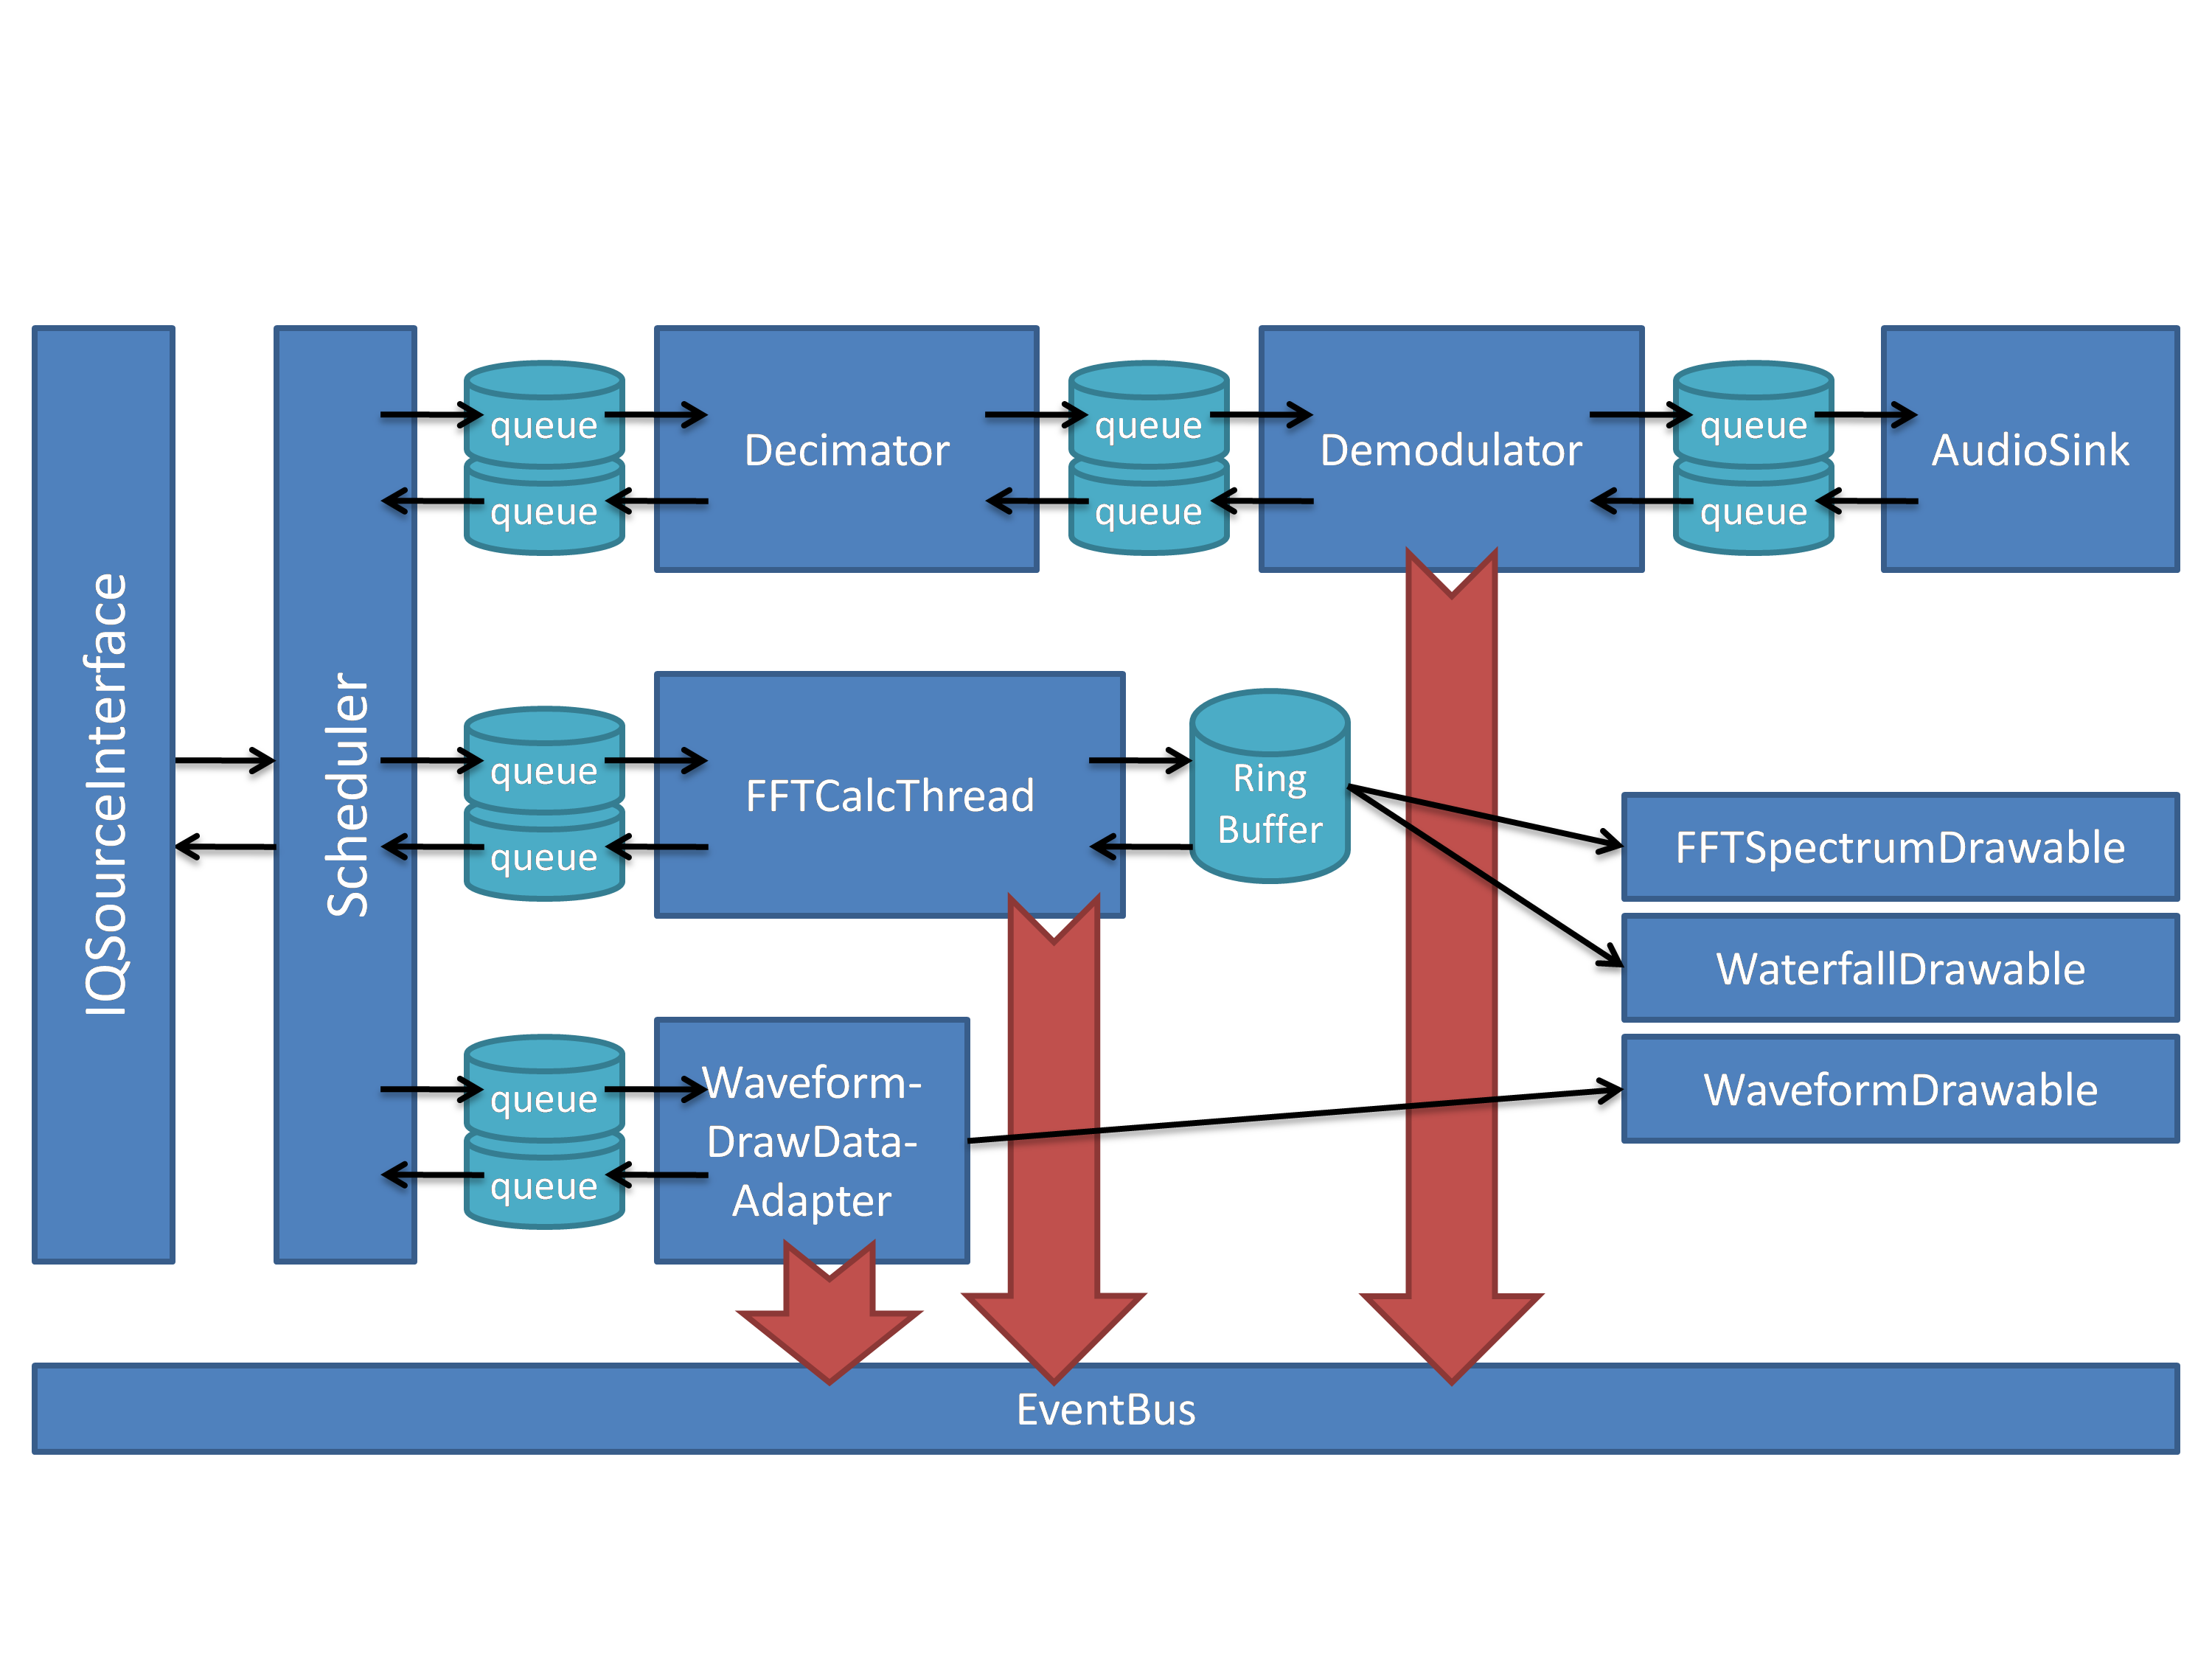
\includegraphics[width=1\linewidth]{gfx/queue_arch}
	\caption{Signal processing architecture with blocking queues}
	\label{fig:queue_architecture}
\end{figure}

The original RF Analyzer application's architecture is based on
blocking queues that synchronize the various signal processing threads
and efficiently manage memory buffers. Unfortunately, this
architecture was partly dropped by the developers of \ac{AnSiAn} when
changing to a new architecture that is based on the EventBus library. As a result, memory
allocation management does not work as efficiently with the original version
of \ac{AnSiAn}.

Instead of using cycling buffers for inter-thread-communication, \ac{AnSiAn} uses
EventBus to deliver data. Buffers are always allocated freshly
and discarded after use. This results in a high activity of the
\ac{GC} and therefore in a bad overall performance of the app.

\autoref{lst:before_mem_optimization} shows a logcat output of the
app before any optimizations were applied. The \ac{GC} runs approximately 8 times per second
and the slow performance results in stuttering audio demodulation on
older hardware.

\begin{lstlisting}[label=lst:before_mem_optimization, caption=Logcat output
before memory optimizations, language=none]
05-12 17:55:04.060 D/dalvikvm: GC_FOR_ALLOC freed 4347K, 14% free 54695K/62984K, paused 28ms, total 28ms
05-12 17:55:04.180 D/dalvikvm: GC_FOR_ALLOC freed 4321K, 14% free 54737K/62984K, paused 26ms, total 26ms
05-12 17:55:04.300 D/dalvikvm: GC_FOR_ALLOC freed 4507K, 14% free 54705K/62984K, paused 32ms, total 32ms
05-12 17:55:04.420 D/dalvikvm: GC_FOR_ALLOC freed 4454K, 14% free 54759K/62984K, paused 30ms, total 30ms
\end{lstlisting}

In order to fix this performance issue, the architecture was reverted
to using blocking queues and cycling buffers in places where large memory buffers are passed
between threads. EventBus is still used to deliver information
which is not tied to large buffers. A schema of the new architecture
is depicted in \autoref{fig:queue_architecture}.

In this architecture, the buffers cycle between the threads. The re-usage
of buffers helps to reduce the memory allocation and garbage collection
overhead to a minimum. \autoref{lst:after_mem_optimization} shows the
logcat output after the architectural changes have been applied. The \ac{GC}
only needs to run every 10 to 20 seconds.


\begin{lstlisting}[label=lst:after_mem_optimization, caption=Logcat output
after memory optimizations, language=none]
05-12 17:27:29.230 D/dalvikvm: GC_FOR_ALLOC freed 3233K, 15% free 19706K/23000K, paused 32ms, total 33ms
05-12 17:27:40.780 D/dalvikvm: GC_FOR_ALLOC freed 3528K, 16% free 20235K/23824K, paused 30ms, total 31ms
05-12 17:28:00.110 D/dalvikvm: GC_FOR_ALLOC freed 4130K, 18% free 20338K/24528K, paused 36ms, total 37ms
05-12 17:28:24.520 D/dalvikvm: GC_FOR_ALLOC freed 4263K, 18% free 20341K/24664K, paused 49ms, total 49ms
\end{lstlisting}

Another significant performance improvement can be achieved by synchronizing
the calculation of the \ac{FFT} to the refresh cycle of the application
\ac{GUI}. This simple change reduces the number of times the \ac{FFT} algorithm
has to be executed and releases processing resources for other calculations
(e.g. the demodulation path). 

Unfortunately, it turned out that the Morse demodulation
algorithm of \ac{AnSiAn} was working in the frequency
domain and relied on continuous \ac{FFT} samples without gaps.
As result, this performance improvement comes at the cost of re-implementing
the Morse demodulation algorithm in order to work on time domain samples
instead.


\section{Demodulation}

This section describes the design and implementation process of the developed demodulation features. \autoref{sec:demod_design} covers where and how the new demodulators and the logging functionality were integrated into the existing architecture and which changes were necessary. Due to performance issues with the old frequency-domain-based Morse demodulator, it had to be re-written. This process is described in \label{sec:morse_demod}. The implementation of the new \ac{RDS} and \ac{PSK31} demodulators is covered in Sections \ref{sec:rds} and \ref{sec:psk31} respectively. \autoref{sec:logging} addresses the implemented logging functionality for demodulator output.


\subsection{Design and Structural Changes\label{sec:demod_design}}

The existing architecture of \ac{AnSiAn} features individual threads for scheduling, 
downsampling, demodulation and audio output. The \texttt{De\-mo\-du\-la\-tor} thread demodulates 
quadrature samples by calling the \texttt{demodulate()} method on an instance of
\texttt{Demodulation}. \texttt{Demodulation} is an abstract class that is implemented by concrete 
demodulation methods such as \texttt{AM}, \texttt{FM} and \texttt{Morse}. 

\ac{AnSiAn} utilizes the EventBus library in order to pass demodulated Morse text
to the \ac{GUI}. Demodulated audio data is passed to the
\texttt{AudioSink} thread by enqueuing it into its input queue.
This mechanism was explained in more detail in \autoref{sec:cleanup.mem}.


In order to extend \ac{AnSiAn} with demodulation functionality for \ac{PSK31} and \ac{RDS}, 
the existing architecture needs to be extended by two new subclasses. The extended architecture is
depicted in \autoref{fig:demod_text_eventbus} and explained in the following.

\begin{figure}
	\centering
	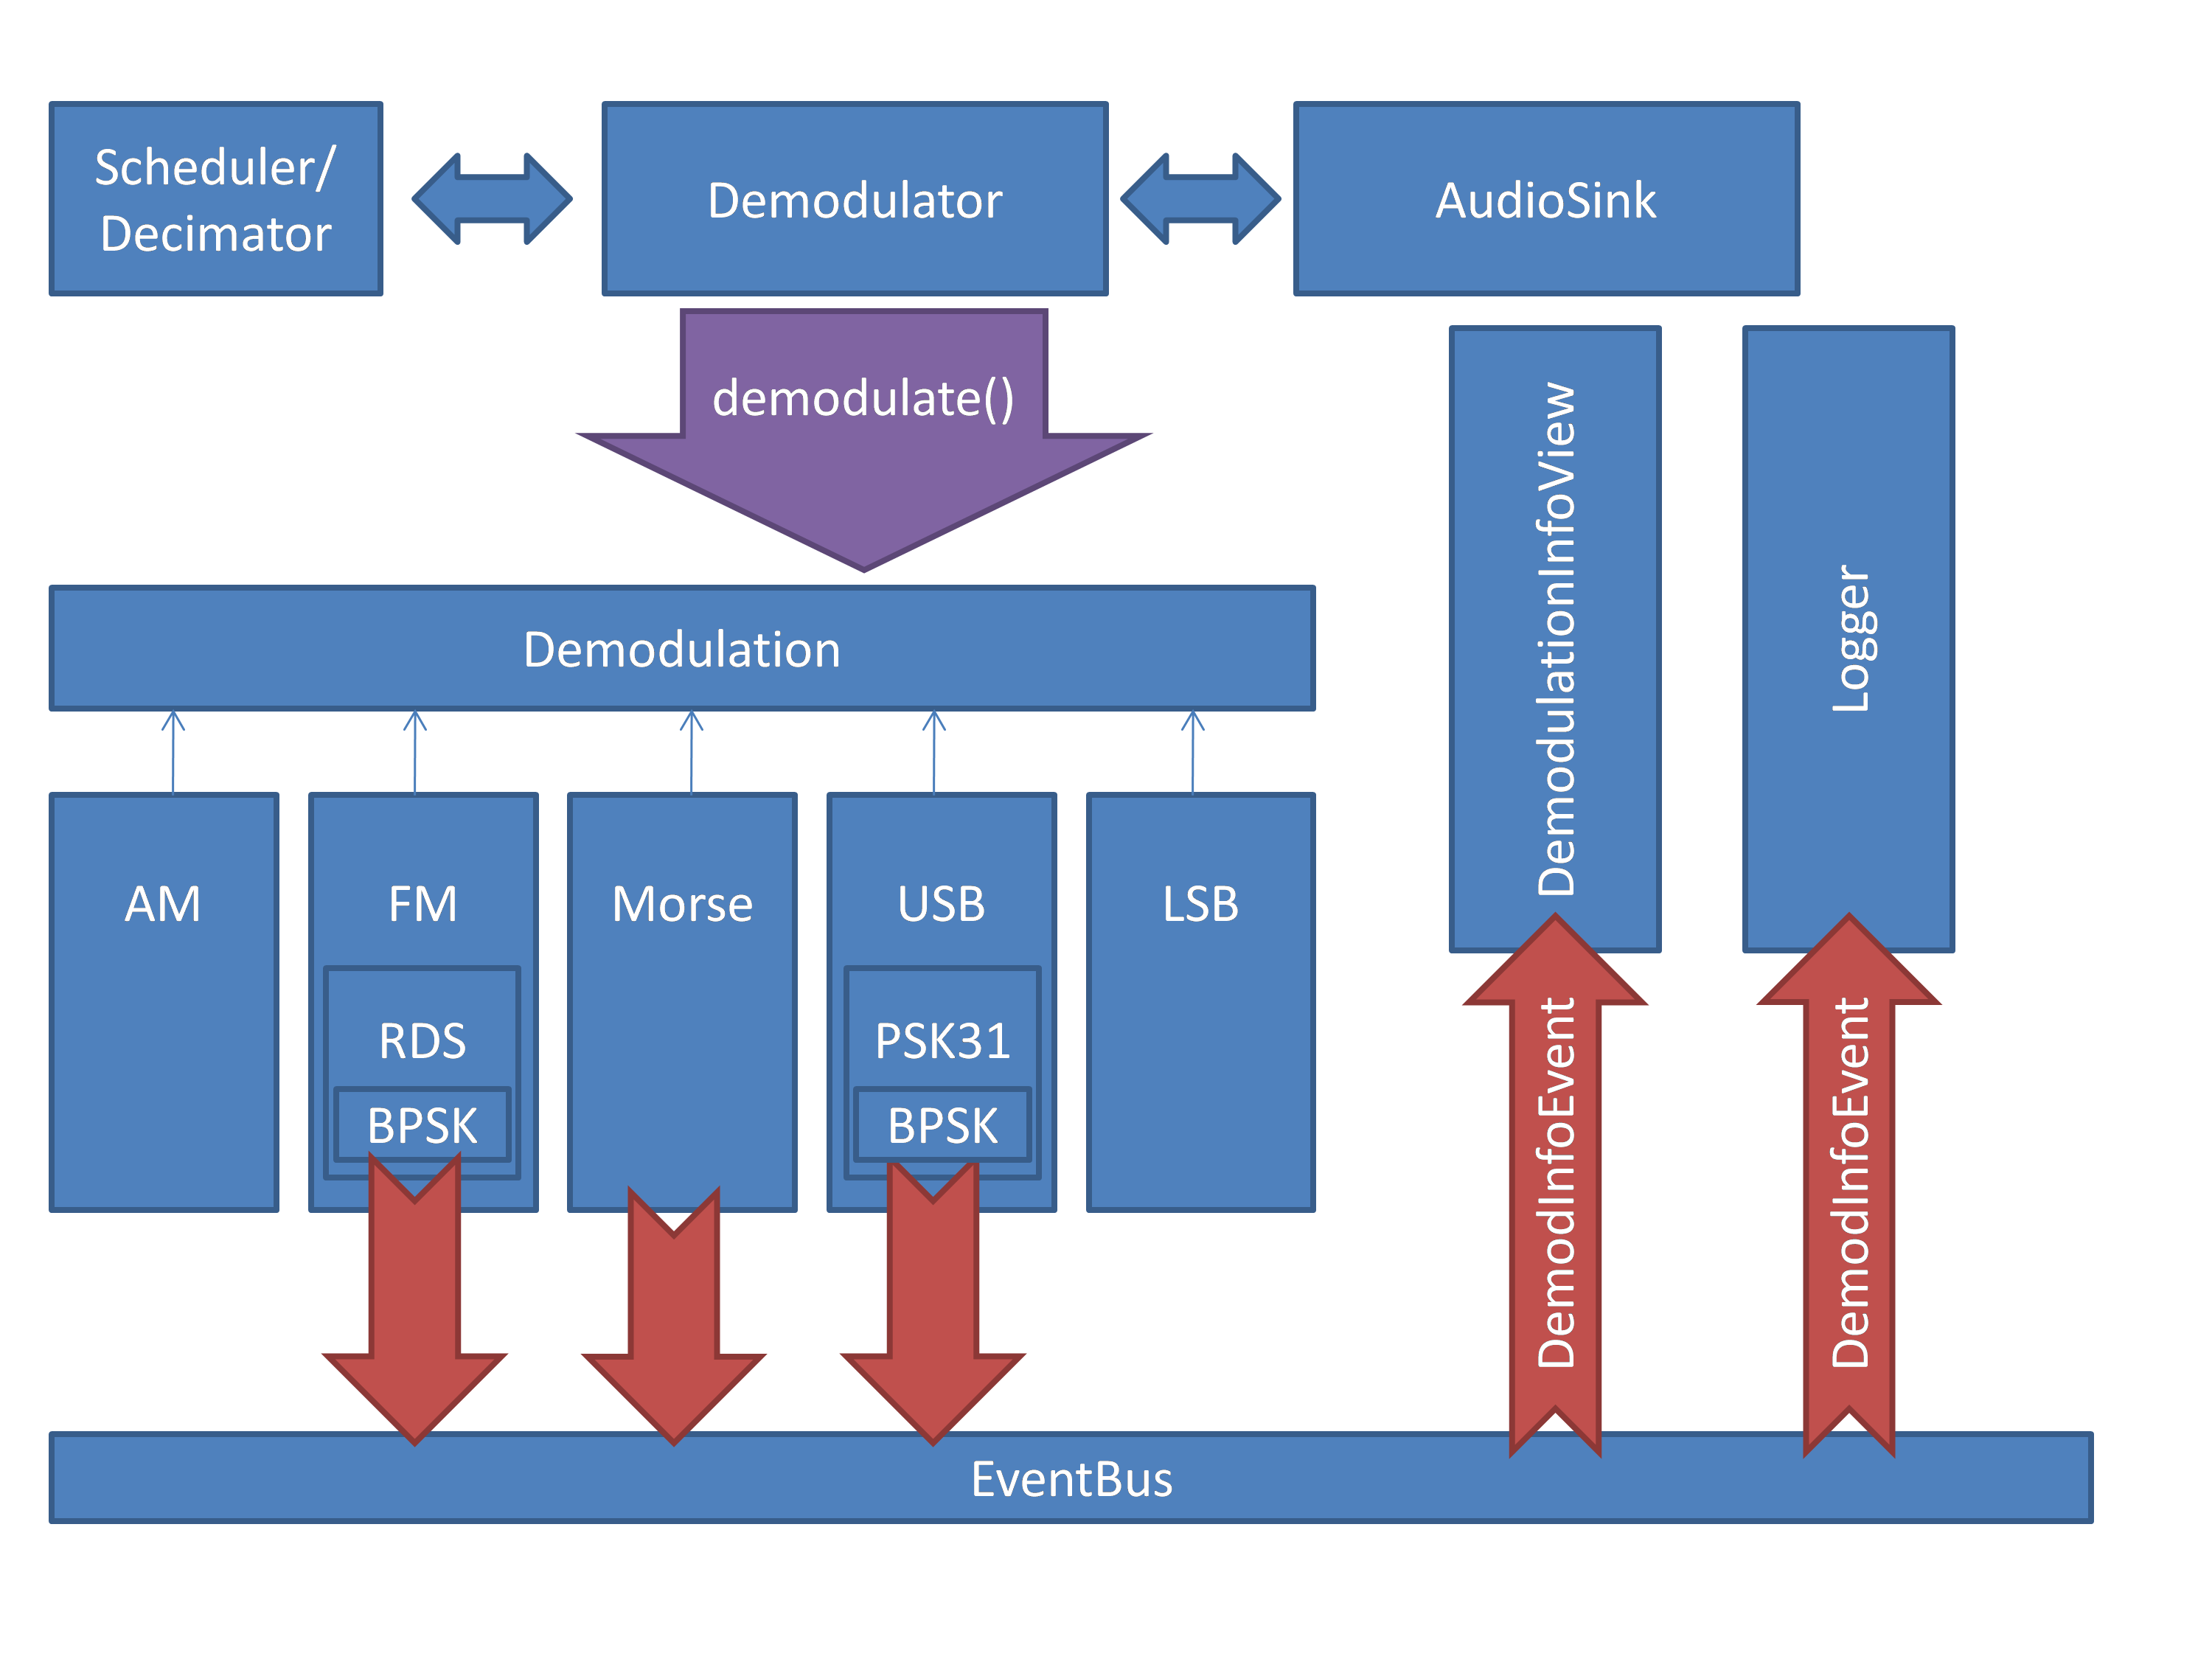
\includegraphics[width=1\linewidth]{gfx/demod_text_eventbus.png}
	\caption{Architecture of the extended demodulation logic and communication with the GUI}
	\label{fig:demod_text_eventbus}
\end{figure}

Two new classes \texttt{PSK31} and \texttt{RDS} are created and instantiated as attributes by the existing demodulation classes for \ac{USB} and \ac{FM}. \ac{PSK31} demodulation
works on the envelope of the received \ac{USB} signal. \ac{RDS} transmits
metadata for \ac{FM} radio channels, which is why the \ac{RDS} demodulation
needs to work on an intermediate result of the wide-band \ac{FM} demodulation
class. Through a new option in the app settings, it is possible to enable
or disable the demodulation of the embedded digital modes when the
corresponding analog mode is selected.

Like the existing architecture, the new architecture uses the EventBus
library to pass the demodulated text to the \ac{GUI}. The existing View
\texttt{MorseReceiveView} is refactored into a universal
\texttt{De\-mo\-du\-la\-tion\-In\-fo\-View} that displays the text output of any selected 
demodulator. Demodulators pass
\texttt{DemodInfoEvent}s via the EventBus to the \texttt{De\-mo\-du\-la\-tion\-In\-fo\-View}, 
which contain demodulated text and further information (e.g. baud rates or raw 
dits and dahs) and are displayed in separate lines.

The new class \texttt{Logger} will also listen for \texttt{DemodInfoEvent}s and, if logfiles for demodulator output are enabled by the user, persist the demodulated data to these logfiles.

\subsection{Re-Implementation of Morse Demodulator\label{sec:morse_demod}}

As explained in \autoref{sec:cleanup.mem}, the original version of \ac{AnSiAn} calculated \acp{FFT} excessively often and thus offered bad performance. \ac{AnSiAn}'s original Morse demodulator, which operated in the frequency domain, relied on frequent \ac{FFT} calculations and did not work after the optimizations described in \autoref{sec:cleanup.mem}. In order to still demodulate Morse with the new efficient architecture, the Morse demodulator needed to be re-written to work in the time domain rather than the computationally expensive frequency domain.

\subsubsection{Requirements}

Aside from demodulating and decoding Morse transmissions, the old demodulator offered support for the following features, which the new demodulator should implement as well.

\begin{itemize}
  \item ``Manual'', ``semi-automatic'' or ``automatic'' detection of dit duration and threshold
  \item Optional automatic re-initialization of detected dit duration and threshold in case of high error rate
  \item Optional \ac{AM} audio demodulation along with Morse demodulation
\end{itemize}

In automatic mode, the demodulator automatically estimates the high/low threshold and the duration of a dit based on a set of samples, that needs to be collected before the actual demodulation can start. Manual mode requires the user to explicitly specify the dit duration and uses the current squelch as threshold. In semi-automatic mode, the user specifies the dit duration while the threshold is determined automatically.

With the new demodulator getting its samples from the \texttt{Decimator} rather than the \texttt{FFTCalcThread}, the practice of using the squelch as threshold is no longer applicable, as samples below the squelch level do not get passed to the \texttt{Demodulator}. The new implementation of the Morse demodulator thus only supports ``automatic'' and ``manual'' mode with respect to dit duration; the threshold is always determined automatically.


\subsubsection{Implementation}

\begin{figure}
	\centering
	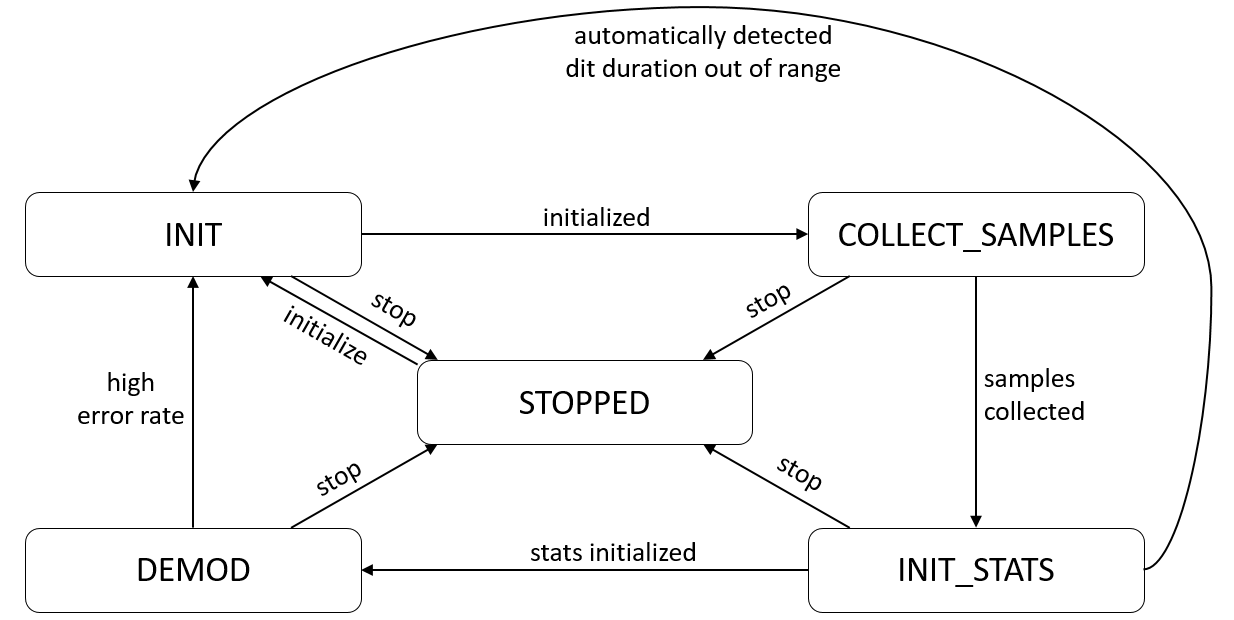
\includegraphics[width=1\linewidth]{gfx/morse_states.png}
	\caption{States and state transitions of the re-written Morse demodulator}
	\label{fig:morse_states}
\end{figure}

The re-written Morse demodulator has five states that are displayed in \autoref{fig:morse_states} and explained in the following.

\paragraph{INIT} In this state, the demodulator initializes its internal state. Samples received while in this state are discarded and not demodulated. In case \ac{AM} demodulation is activated, audio still is demodulated.
\paragraph{COLLECT\_{}SAMPLES} The demodulator calculates and stores the envelope of all received samples in a buffer. In case \ac{AM} demodulation is activated, audio is demodulated.
\paragraph{INIT\_{}STATS} The collected samples from the previous state are used to initialize the threshold and, optionally, the dit duration. Samples received while in this state are discarded and not demodulated. In case \ac{AM} demodulation is activated, audio still is demodulated.
\paragraph{DEMOD} Received samples are demodulated on-the-fly. If demodulation or decoding error rates are beyond a threshold, the demodulator re-initializes.
\paragraph{STOPPED} The demodulator should not be running; all samples are discarded.
\paragraph{}

For envelope detection, $\sqrt{I^{2}+Q^{2}}$ is used, with $I$ and $Q$ being the inphase and quadrature components of the sample, respectively. This is computationally more expensive than using the existing \ac{AM} demodulator to detect the envelope, but produces more exact results and comes without the unwanted automatic gain control of the \ac{AM} demodulator. For efficient memory management, the envelope of the currently processed sample packet is not always stored in a new array. Instead, a buffer is allocated once and overwritten with the current envelope each time a new sample packet is processed. If \ac{AM} demodulation is enabled, the envelope is copied from the buffer to the demodulator output, which is passed to the \texttt{AudioSink}.

The threshold, that determines whether a given sample is a ``low'' or a ``high'' sample (i.e. if it is part of a dit/dah or a pause), is initialized based on the initialization data collected during the COLLECT\_{}SAMPLES step and continuously updated for every processed sample. It is calculated as $bottom + \frac{peak - bottom}{2}$, with $bottom$ being the lowest and $peak$ being the highest amplitude seen since the demodulator's initialization.

If automatic mode is enabled, the dit duration is determined by counting streaks of consecutive ``high'' (i.e. bigger than the threshold) samples in the initialization data. The observed streak lengths are then adjusted by adding the number of observed streaks with one sample more or less (i.e. $o_{new}(x) = o(x-1) + o(x)+ o(x+1)$ with $o(x)$ being the number of occurrences of a continuous high-streak of $x$ samples). This is done to cope with outliers. The most frequently observed streak length is assumed to be the number of samples per dit. If this number of samples corresponds to less than \SI{7}{\milli\second} of samples, it is assumed that the initialization data was of poor quality and the demodulator reinitializes itself.

In DEMOD state, streaks of continuous high and low values in the currently processed samples packet are counted. The length of a streak and its value (i.e. high or low) are then decoded to find out whether it encodes a dit, dah or a short, medium or long pause. If a medium pause (encodes the end of character symbol) is detected, the previous dits and dahs are passed to the \texttt{Decoder} class, which translates them into a character. The \texttt{Decoder} class was already used by the old demodulator. It was originally taken from the open-source project Morsecoder and recycled for the new Morse demodulator.

To implement automatic re-initialization, the demodulator uses \texttt{Er\-ror\-Bit\-Set}s, which are essentially ring buffers for boolean values. Two \texttt{Er\-ror\-Bit\-Set}s are used; one for demodulation (i.e. translating streak lengths into dits, dahs and pauses) and one for decoding (i.e. translating dits and dahs into characters). Every entry represents a successful or unsuccessful decoding/demodulation attempt. The size of the \texttt{Er\-ror\-Bit\-Set} that tracks demodulation success is 100, the size for the decoding success \texttt{Er\-ror\-Bit\-Set} is 30. If the success rate drops below 50\%, the demodulator re-initializes itself and thus re-determines the threshold and, if automatic mode is enabled, dit duration.


\autoref{lst:morse_demod_method} shows an excerpt of the demodulator's core method \texttt{de\-mo\-du\-late()}. The operation of the demodulator, as described in this section, can be recognized in it.

\begin{lstlisting}[label=lst:morse_demod_method, caption=The demodulate method of the new Morse demodulator (excerpt), language=java]
switch (this.state) {
    case INIT:
        if (amDemod) {
            // do nothing except AM Demodulation; Demodulator might be in inconsistent state
            envelopeToBuffer(input);
            amDemodFromBuffer(output);
        }
        break;
    case COLLECT_SAMPLES:
        // collect samples and write them to initSamples until we have enough
        envelopeToBuffer(input);
        if (amDemod)
            amDemodFromBuffer(output);
        collectSamplesFromBuffer();
        if (!(initSamplesCollected < initSamplesRequiredForInit))
            initializeStats();
        break;
    case INIT_STATS:
        if (amDemod) {
            // do nothing except AM Demodulation; Demodulator might be in inconsistent state
            envelopeToBuffer(input);
            amDemodFromBuffer(output);
        }
        break;
    case DEMOD:
        // demodulate samples
        envelopeToBuffer(input);
        if (amDemod)
            amDemodFromBuffer(output);
        updateThresholdFromBuffer();
        binarizeBuffer();
        demodulateBuffer();
        if (automaticReinit && needsReinit())
            init();
        break;
    case STOPPED:
        // discard samples; Demodulator should not be running
}
\end{lstlisting}

A screenshot of the running Morse demodulator can be seen in \autoref{fig:morse_screenshot_new}.

\begin{figure}[h]
	\centering
	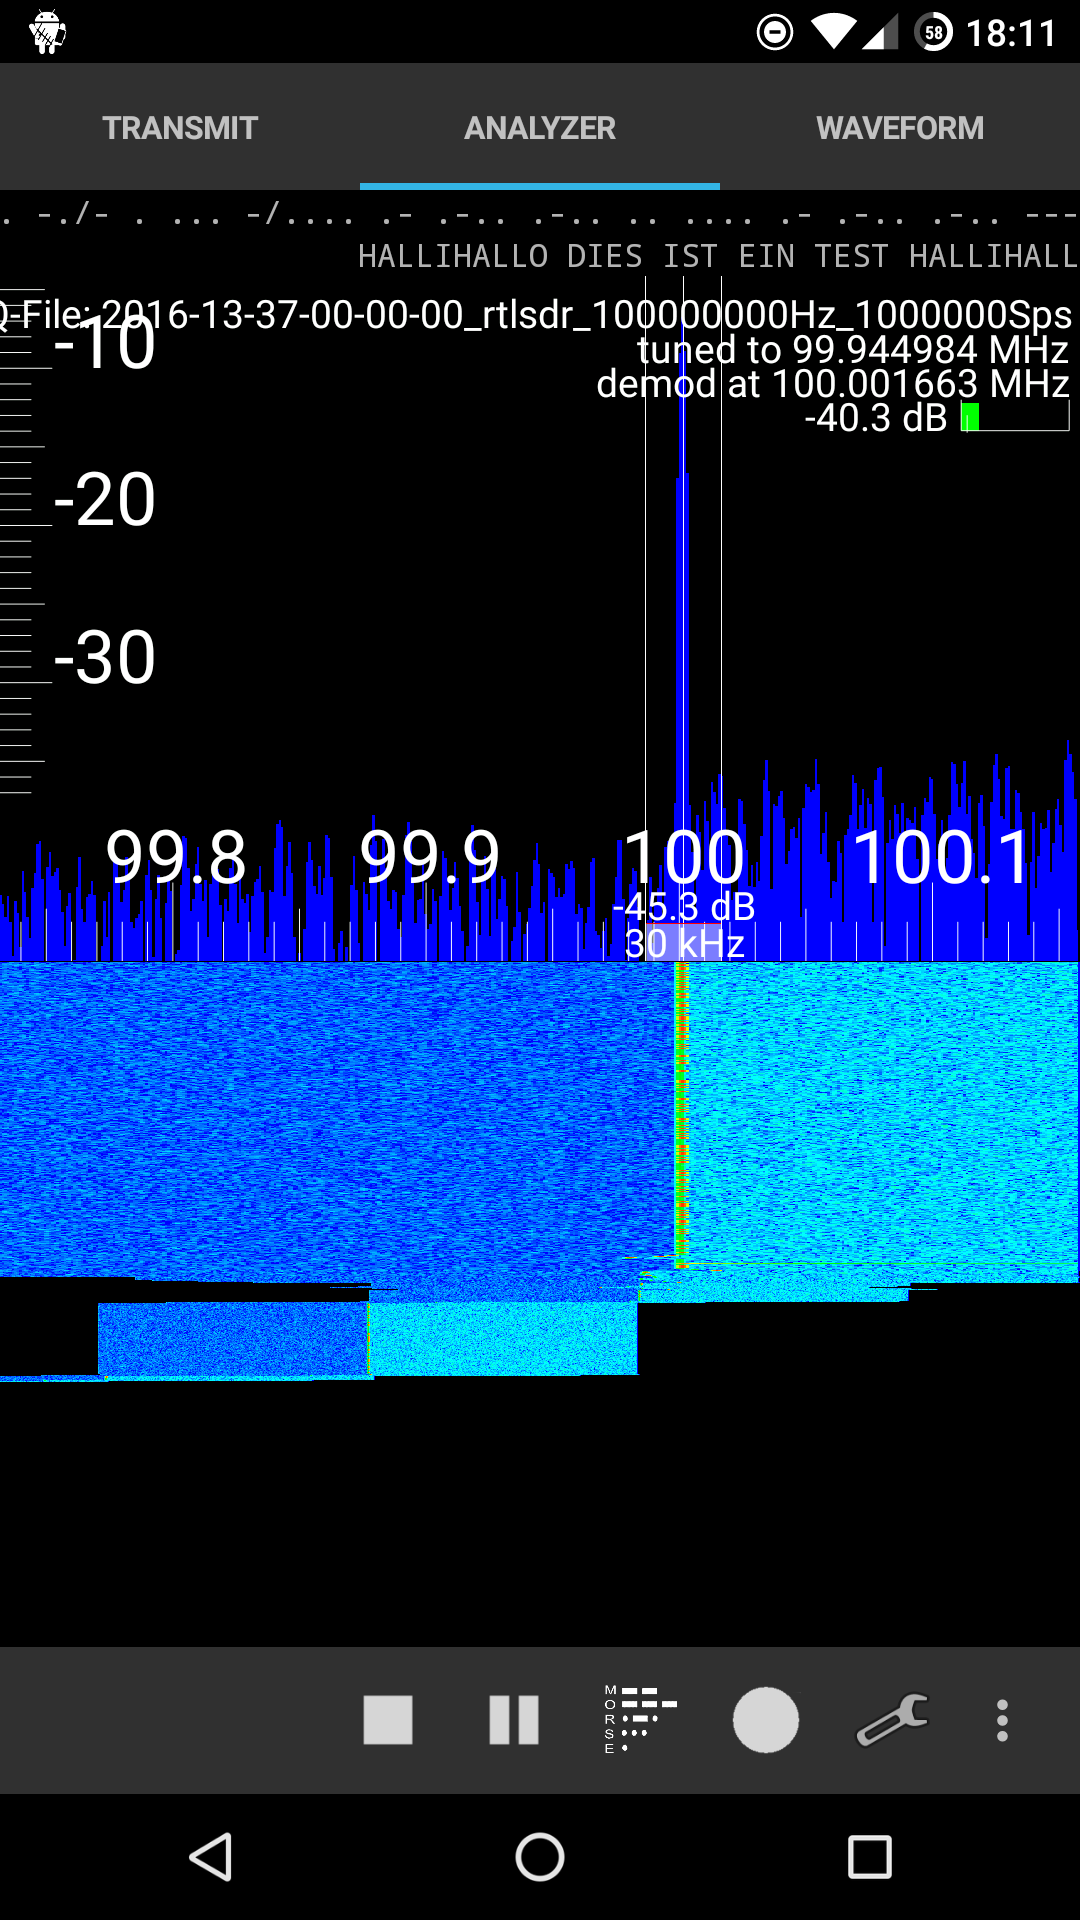
\includegraphics[width=0.5\linewidth]{gfx/screenshots/morse_screenshot_new.png}
	\caption{Screenshot of the Morse demodulator on a Nexus 5X}
	\label{fig:morse_screenshot_new}
\end{figure}



\subsection{Radio Data System \label{sec:rds}}

The \ac{RDS} signal is transmitted along with wide band \ac{FM}
radio signals to provide additional information about the
radio station and program.

Demodulation of the \ac{RDS} signal is first done in Octave in order to
evaluate the demodulation algorithm. The octave implementation
also helps by providing reference data of the different stages
of demodulation. 

\subsubsection{RDS modulation scheme}
\label{sec:rds_modulation_scheme}

\ac{RDS} uses \ac{BPSK} with Manchester encoding. The signal is
transmitted with an offset of 57 kHz relative to the center frequency
of the mono audio signal (baseband). The 19 kHz pilot tone of wideband \ac{FM}
can therefore be used to retrieve the \ac{RDS} carrier by multiplying
it with itself 3 times. The complete FM spectrum can be seen in
\autoref{fig:quad_demod_spectrum}.

After the \ac{RDS} baseband signal has been retrieved from the \ac{FM} signal
there are multiple ways of demodulating the \ac{BPSK} modulation. A sophisticated
approach tries to recover the phase synchronized \ac{RDS} carrier from the
signal by using e.g. a form of \ac{PLL} or Costas Loop. The symbols can then
be extracted by multiplying the carrier with the modulated signal and apply
a threshold operation to get bits.

A much simpler approach is to analyze the envelope of the signal and detect
bits based on known shapes of ones and zeros in the waveform.
\autoref{fig:rds_envelope} shows the envelope and the pattern of symbols
which can be detected.

\begin{figure}
	\centering
	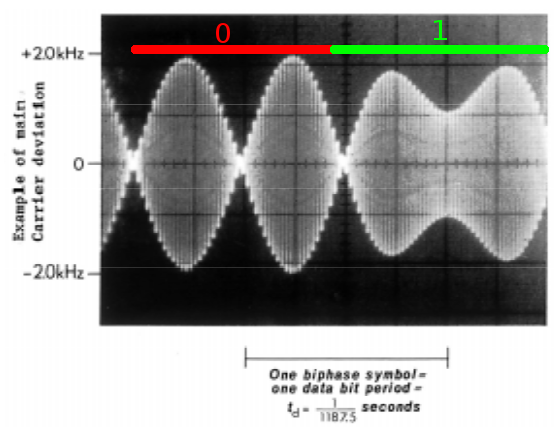
\includegraphics[width=1\linewidth]{gfx/rds/rds_waveform.png}
	\caption[RDS envelope waveform after Frequency demodulation]{RDS envelope waveform after Frequency demodulation \cite{1999:iec62106}}
	\label{fig:rds_envelope}
\end{figure}



\subsubsection{RDS coding scheme}

RDS frames are called groups and each group consists of 4 blocks called
A, B, C and D. One block has a length of 16 bit plus a 10 bit checkword.
Block A always contains the \ac{PI} which identifies the radio station.
The content of the other blocks depends on the group type which is located
in block B (see \autoref{fig:rds_group0A}).

\begin{figure}
	\centering
	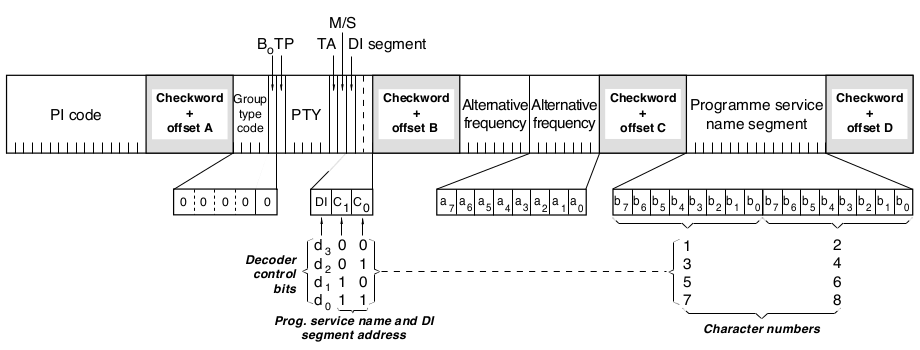
\includegraphics[width=1\linewidth]{gfx/rds/group0A.png}
	\caption[Coding scheme of RDS: group 0A]{Coding scheme of RDS: group 0A \cite{1999:iec62106}}
	\label{fig:rds_group0A}
\end{figure}

\autoref{tab:rds_groups} (see appendix) lists all group types and their descriptions.
The \ac{RDS} demodulation in AnSiAn only decodes types 0 and 2 because they contain
the basic information which is also often displayed on the radio
receiver.


\subsubsection{Evaluation in Octave}

Developing a signal processing application on Android has many drawbacks. One
issue is that it is very hard to debug the actual signal processing components
because of the lack of proper tools to visualize and analyze the data that is
being processed. It is also not possible to do rapid prototyping without
sufficient signal processing libraries available. Therefore, the \ac{RDS}
demodulator was first developed in Octave and afterwards ported to Android.

For development and testing it is better to work on recorded samples instead
of live captures. This makes tests reproducible and simplifies the development
environment. The file was recorded using the record feature of RF Analyzer. It
can be imported in Octave by using the \texttt{read\_cuchar\_binary()} script
provided by the GNU Radio project. After each step the produced output data
can be written back to an \emph{IQ} file in order to use it in the Android application.
This way it is possible to develop each component of the demodulation process
separately and the output can be visualized on the developing machine.

The demodulation is done in the following steps:
\begin{enumerate}
	\item Downmixing the radio signal to baseband and filter it (see 
		\autoref{fig:rds_downmixing}).
	\item \ac{FM} demodulation (see \autoref{fig:quad_demod_spectrum}).
	\item Downmixing the \ac{RDS} signal to baseband and filter it
		(see \autoref{fig:rds_extraction} b and c).
	\item Take the absolute value of the signal to get the envelope
		that was shown above (see \autoref{fig:rds_waveform}).
	\item Find the beginning of a symbol by searching for a minimum in
		the waveform. From there find the end of the symbol with the
		same strategy. Now determine whether the symbol is a one or a
		zero according to the value of the minimum found in the middle
		of the sample compared to its peaks.
\end{enumerate}

\begin{figure}
\subfloat[Spectrum of the captured signal]{%
  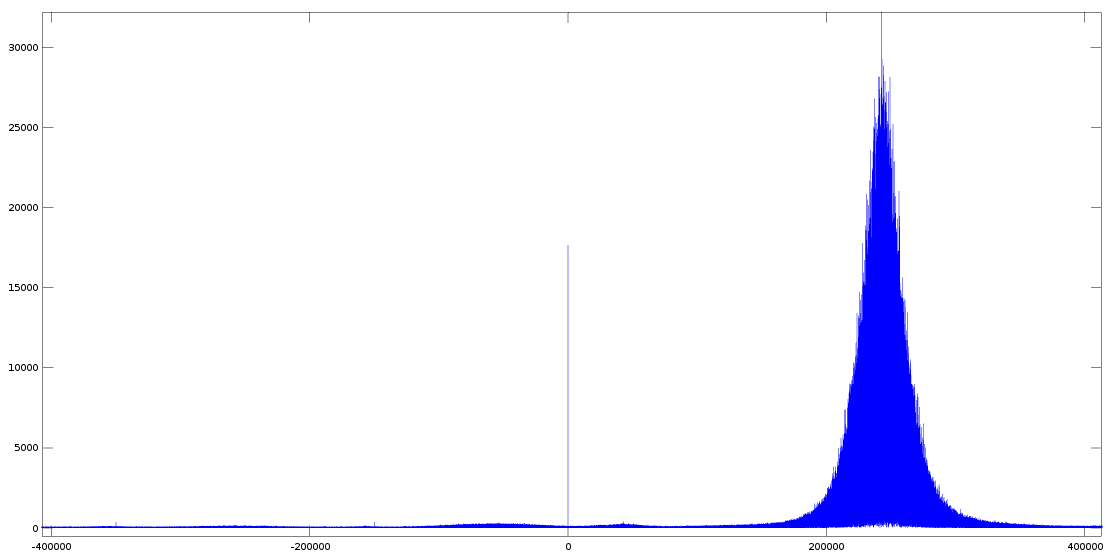
\includegraphics[clip,width=1\linewidth]{gfx/rds/raw_signal_spectrum.png}%
}

\subfloat[Spectrum after downmixing and filtering]{%
  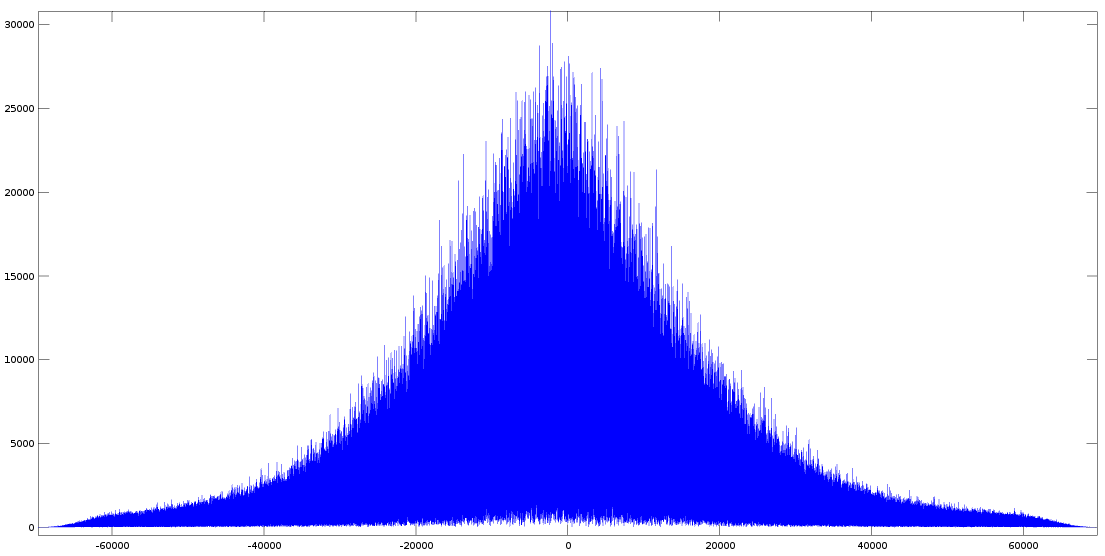
\includegraphics[clip,width=1\linewidth]{gfx/rds/fm_baseband_filtered_spectrum.png}%
}
\caption{FM Modulated Signal}
\label{fig:rds_downmixing}
\end{figure}


\begin{figure}
\subfloat[Signal spectrum after FM demodulation]{%
  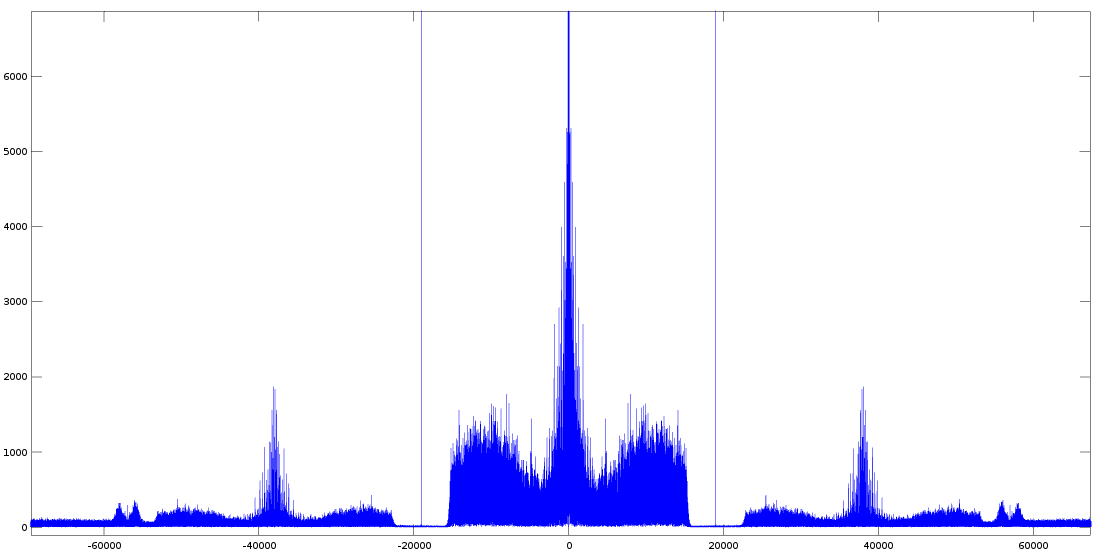
\includegraphics[clip,width=1\linewidth]{gfx/rds/quad_demod_spectrum.png}%
  \label{fig:quad_demod_spectrum}
}

\subfloat[RDS baseband spectrum after downmixing]{%
  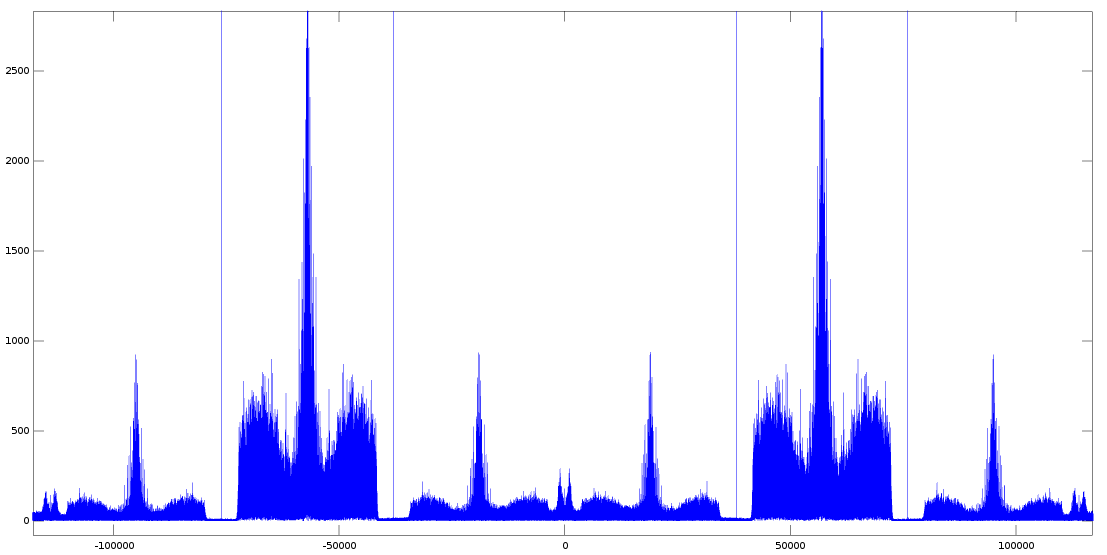
\includegraphics[clip,width=1\linewidth]{gfx/rds/rds_baseband_unfiltered_spectrum.png}%
}

\subfloat[RDS baseband spectrum after filtering]{%
  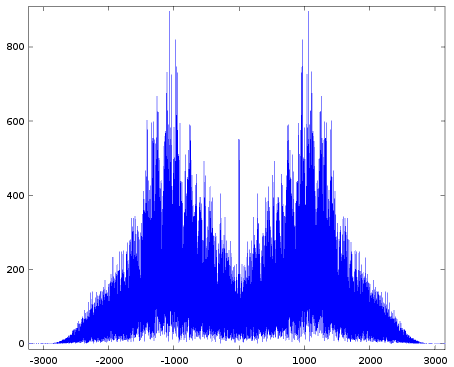
\includegraphics[clip,width=1\linewidth]{gfx/rds/rds_baseband_spectrum.png}%
}
\caption{Extracting the RDS signal from the FM signal}
\label{fig:rds_extraction}
\end{figure}

\begin{figure}
	\centering
	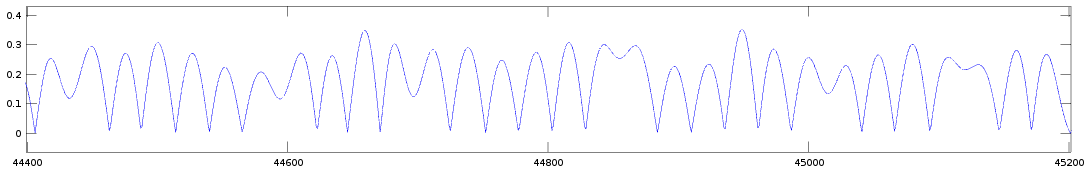
\includegraphics[width=1.1\linewidth]{gfx/rds/rds_magnitude_waveform.png}
	\caption{RDS waveform after take the absolute values}
	\label{fig:rds_waveform}
\end{figure}

The octave code used to execute the steps mentioned above is shown in the
listing below:

\begin{lstlisting}[label=lst:octave_rds, caption=Octave implementation of the RDS demodulator, language=octave]
signal = read_cuchar_binary ("rtlsdr_100550000Hz_1000000Sps.iq");
t = linspace(0, length(signal)/1000000, length(signal))';
carrier = e.^(2*pi*-245000*t*i);
down = carrier .* signal;
fl = fir1(300, 100000/1000000*2);
filtered = filter(fl, 1, down);
demod = quad_demod(filtered, 1);
t2 = linspace(0, length(demod)/1000000, length(demod));
rdscarrier = cos(2*pi*-57000*t2)';
rdsbase = demod(1:length(rdscarrier)) .* rdscarrier ;
frds = fir1(300, 2400/1000000*2);
rdsbase_filtered = filter(frds,1,rdsbase);
downsampled = decimate(rdsbase_filtered, 16).*80;
write_cuchar_binary (downsampled, "rds_baseband_62500sps.iq");
bits = rds_bpsk_demodulate(downsampled, 62500);
rds_decode(bits)
\end{lstlisting}

The \texttt{quad\_demod()} function does the quadrature demodulation
(FM demodulation). The \texttt{rds\_bpsk\_demodulate()} function is shown
in the following listing:

\begin{lstlisting}[label=lst:octave_rds_bpsk, caption=Octave implementation of the BPSK demodulation, language=octave]
function demod = rds_bpsk_demodulate(signal, fs)
  samples_per_symbol = fs/1187.5
  samples_per_symbol = ceil(samples_per_symbol)
  envelope = abs(signal);
  
  % Find the first minimum
  [minimum, idx1] = min(envelope(1:samples_per_symbol))
  
  bits = [];
  while (idx1 + samples_per_symbol*2 < length(envelope))
    % find end of symbol idx2 (minimum near idx1 + samples_per_symbol)
    from = round(idx1+samples_per_symbol*0.75);
    to   = round(idx1+samples_per_symbol*1.25);
    [minimum, idx2] = min(envelope(from:to));
    idx2 = idx2 + from;
    
    % calc mean of all samples between idx1 and idx2 and calc threshold = mean/2
    m = mean(envelope(idx1:idx2));
    threshold = m/2;
    
    % get minimum sample in the middle between idx1 and idx2 ...
    span = idx2 - idx1;
    from = round((idx1+idx2)*0.5 - 0.25*span);
    to   = round((idx1+idx2)*0.5 + 0.25*span);
    [minimum, idxmiddle] = min(envelope(from:to));
    idxmiddle = idxmiddle + from;
    
    % Check whether we have the correct timing. It might be, that idx2 is
    % actually in the middle of a symbol than at its end.
    if (envelope(idx2) > threshold)
      % In this case we find the minimum between idx1 and idx2 and set it
      % as idx1 for the next round:
      %printf("WARNING: Wrong timing. thres=%f < envelope(idx2=%d)=%f\n",threshold,idx2,envelope(idx2));
      idx1 = idxmiddle;
      continue;
    endif
    
    % ... and check it against the threshold
    s = envelope(idxmiddle);
    if (s > threshold)
      bits = [bits 1];
    else
      bits = [bits 0];
    endif
    
    % idx1 = idx2 and continue with the next symbol..
    idx1 = idx2;
    
  endwhile
  demod = bits;
\end{lstlisting}


\subsubsection{Android Implementation}

For the Android implementation two classes are added to the AnSiAn codebase:
\begin{itemize}
	\item \texttt{BPSK}: This class handles the \ac{BPSK} demodulation and can be
		reused by other demodulators using the \ac{BPSK} modulation scheme
		(e.g. PSK31).
	\item \texttt{RDS}: This class integrates in the existing FM class for frequency
		demodulation. It handles the decoding and processing of \ac{RDS}
		groups. 
\end{itemize}

A screenshot of the application demodulating the \ac{RDS} signal of the
\emph{Antenne Frankfurt} station is shown in \autoref{fig:rds_android_screenshot}.

\begin{figure}
	\centering
	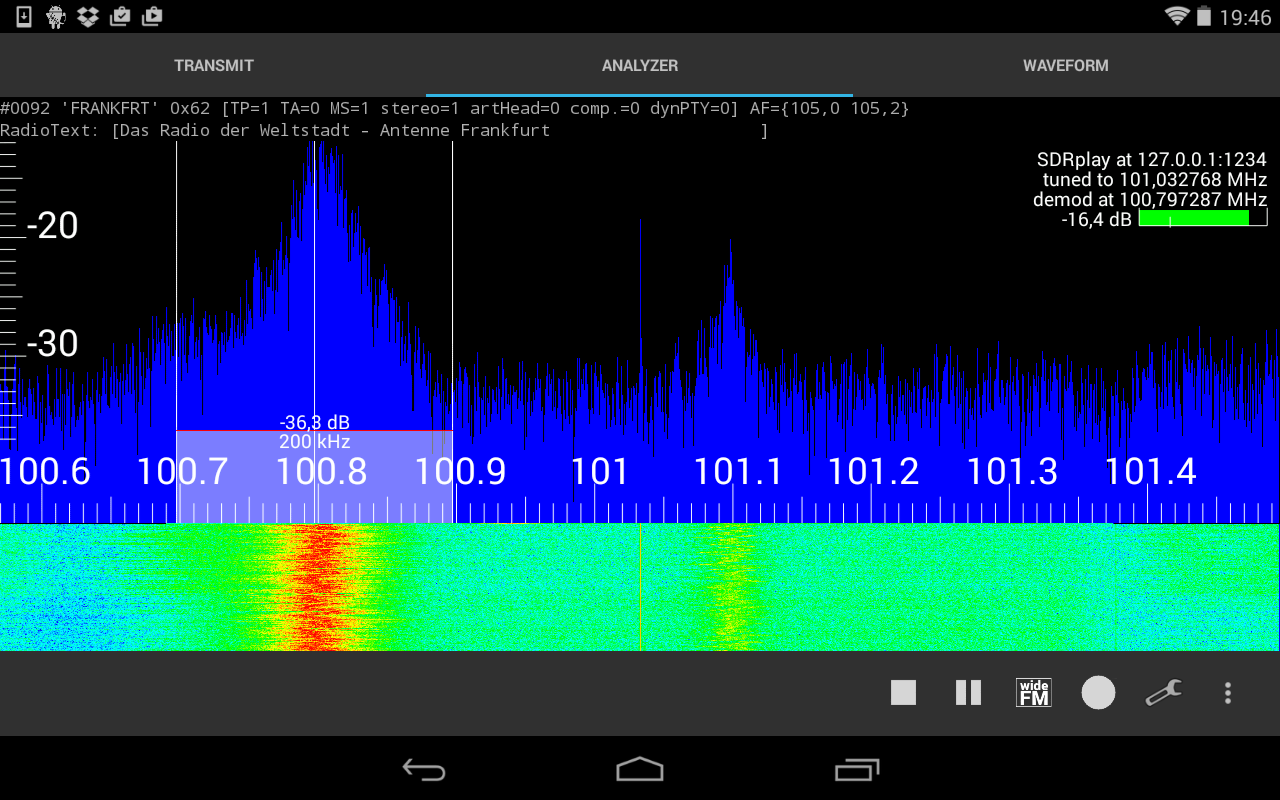
\includegraphics[width=1\linewidth]{gfx/rds/android_screenshot.png}
	\caption{Screenshot of the RDS demodulator on a Nexus 7}
	\label{fig:rds_android_screenshot}
\end{figure}


\subsection{PSK31\label{sec:psk31}}

\ac{PSK31} refers to phase shift keying modulation using a baud rate of 31.25
Hz.  It was developed by Peter Martinez in 1998 to introduce a narrow bandwidth
digital mode for live chatting \cite{martinez1998psk31}. Because of the simple and efficient modulation
and coding scheme (e.g. it does not have an error correction mechanism) it is
very widespread amongst amateur radio operators.

A typical setup for \ac{PSK31} operation is a \ac{SSB} transceiver connected
to the sound card of a computer. The audio channel that is fed into the computer
can contain multiple parallel \ac{PSK31} transmissions, which are demodulated
using a special software.

PSK31 is usually operated in \ac{USB} mode and shall therefore be available
in \ac{AnSiAn} when the \ac{USB} demodulator is active.
As with the \ac{RDS} demodulator the algorithm to demodulate and decode \ac{PSK31}
is first evaluated in Octave and later ported to the \ac{AnSiAn} application.

\subsubsection{PSK31 modulation scheme}

\ac{PSK31} in its basic form uses \ac{BPSK} to transmit binary information by
sending a single side band signal with either a 180 degree phase shift (digital
'1') or without a phase shift (digital '0'). Additionally, a root raised cosine
filter is used in order to smooth the phase shift and therefore keep the
bandwidth narrow.  Each symbol contains information about one bit and is always
32 ms long.

\autoref{fig:psk31_modulation} shows the modulated \ac{PSK31} signal. As already
explained in \autoref{sec:rds_modulation_scheme}, the signal may be demodulated
by using a second order loop (e.g. a Costas loop) in order to recover the phase
information and correct for small frequency variations. However, the simple approach
using envelope detection is also possible. The \ac{BPSK} code used for \ac{RDS}
demodulation can be partly reused and only needs some modifications as \ac{PSK31}
does not use Manchester Encoding.

\begin{figure}
	\centering
	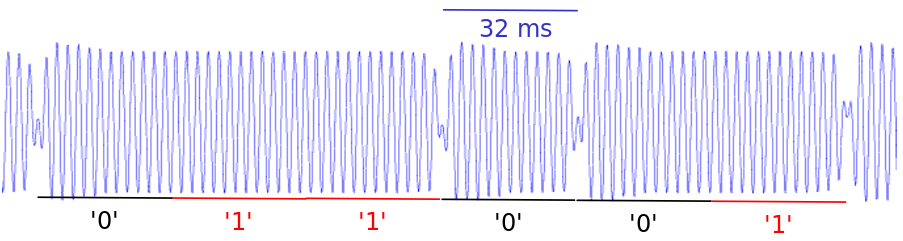
\includegraphics[width=1\linewidth]{gfx/psk31/psk31_modulation.png}
	\caption{PSK31 modulation scheme: Each symbol is 32ms long. A 180° phase
	shift indicates a '0', no phase shift indicates a '1'}
	\label{fig:psk31_modulation}
\end{figure}

\subsubsection{PSK31 coding scheme}

\ac{PSK31} uses a variable length encoding called \emph{Varicode} which assigns
frequently used characters a shorter code similar to Morse. Characters are separated
by two consecutive zeros. \autoref{tab:psk31_varicode} in the appendix lists all
characters and their varicode encodings.

\subsubsection{Evaluation in Octave}

The demodulation algorithm in octave comprises the following steps:
\begin{enumerate}
	\item Downmixing the \ac{USB} signal to baseband.
	\item \ac{USB} demodulation (complex bandpass filter to
		get only the upper side band). See \autoref{fig:psk31_signal_spectrum} b.
	\item Downsampling in order to reduce the workload for the PSK31 demodulation.
	\item Envelope detection. See \autoref{fig:psk31_envelope}.
	\item Find the beginning of a '0' symbol by searching for a minimum in the
		envelope of the signal. Determine whether the next symbol is a '0' (another
		minimum is found around 32ms from the beginning of the current symbol) or
		a '1' (no minimum at the beginning of the next symbol). If another '0' was
		detected, the timing can be corrected by centering the minimum at the beginning
		of the signal and search on from there.
\end{enumerate}

\begin{figure}
\subfloat[Raw spectrum. The PSK31 signal is at around 55 KHz.]{%
  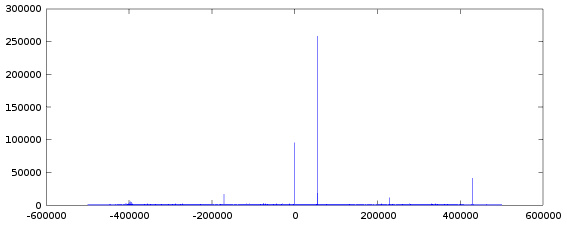
\includegraphics[clip,width=1\linewidth]{gfx/psk31/psk31_raw_signal.png}%
}

\subfloat[Spectrum after downmixing and filtering (USB demodulation)]{%
  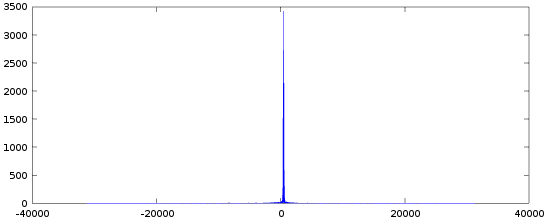
\includegraphics[clip,width=1\linewidth]{gfx/psk31/psk31_usb_demod.png}%
}
\caption{PSK31 signal in the frequency domain (spectrum)}
\label{fig:psk31_signal_spectrum}
\end{figure}

\begin{figure}
	\centering
	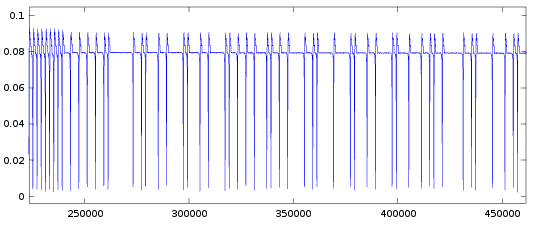
\includegraphics[width=1\linewidth]{gfx/psk31/psk31_envelope.png}
	\caption{Envelope of the downsampled, USB demodulated signal.}
	\label{fig:psk31_envelope}
\end{figure}

The octave code used to execute the steps mentioned above is shown in the
listing below:

\begin{lstlisting}[label=lst:octave_psk31, caption=Octave implementation of the PSK31 demodulator, language=octave]
% load signal
signal = read_cuchar_binary ("rtlsdr_434570917Hz_1000000Sps.iq");
fs = 1000000;

% downmixing (signal is at ~ 55 Khz)
fc = 55000;
t = linspace(0, length(signal)/fs, length(signal))';
carrier = e.^(2*pi*-fc*t*i);
down = carrier .* signal;

% USB demod (bandpass filter [200Hz-1000Hz])
bpfilter = firls(300, [0 200 200 1000 1000 fs/2]./(fs/2), [0 0 0 1 0 0]);
filtered = filter(bpfilter, 1, down);

% downsampling
downsampled = decimate(filtered, 16);

% BPSK demodulation
bits = psk31_bpsk_demodulate(downsampled, fs/16);

% Varicode decoding
psk31_decode(bits)
\end{lstlisting}

The \texttt{psk31\_bpsk\_demodulate()} function is shown in the following listing:

\begin{lstlisting}[label=lst:octave_psk31_bpsk, caption=Octave implementation of the BPSK demodulation, language=octave]
function demod = psk31_bpsk_demodulate(signal, fs)
  % PSK31 baud rate is 31.25 Hz
  samples_per_symbol = fs/31.25
  samples_per_symbol = ceil(samples_per_symbol)
  envelope = abs(signal);
  
  % Find the first minimum
  [minimum, idx1] = min(envelope(1:samples_per_symbol))
  
  bits = [];
  while (idx1 + samples_per_symbol*2 < length(envelope))
    % search for a minimum at the position of the next sample
    % (minimum near idx1 + samples_per_symbol)
    from = round(idx1+samples_per_symbol*0.5);
    to   = round(idx1+samples_per_symbol*1.5);
    [minimum, idx2] = min(envelope(from:to));
    idx2 = idx2 + from;
    
    % calc mean of all samples between idx1 and idx2 and calc threshold = mean/2
    m = mean(envelope(idx1:idx2));
    threshold = m/2;
    
    % Check whether we have a minimum (->0) or not (->1).
    if (envelope(idx2) > threshold)
      % In this case we have a bit 1.
      bits = [bits 1];
      idx1 = idx1 + samples_per_symbol;
    else
      % In this case we have a bit 0.
      bits = [bits 0];
      idx1 = idx2;
    endif
  endwhile
  demod = bits;
\end{lstlisting}

\subsubsection{Android Implementation}

For the Android implementation the \texttt{BPSK} class is modified to handle both
\ac{BPSK} variations needed in \ac{AnSiAn}:
\begin{itemize}
	\item RDS: BPSK with Manchester and Differential Encoding
	\item PSK31: BPSK without Manchester Encoding
\end{itemize}

Additionally, the class \texttt{PSK31} is added which is a subclass of \texttt{De\-mo\-du\-la\-tion}.
It integrates with the existing \texttt{USB} class to provide PSK31 demodulation
when USB demodulation is active.

A screenshot of the application demodulating a \ac{PSK31} signal is shown in 
\autoref{fig:psk31_android_screenshot}.

\begin{figure}
	\centering
	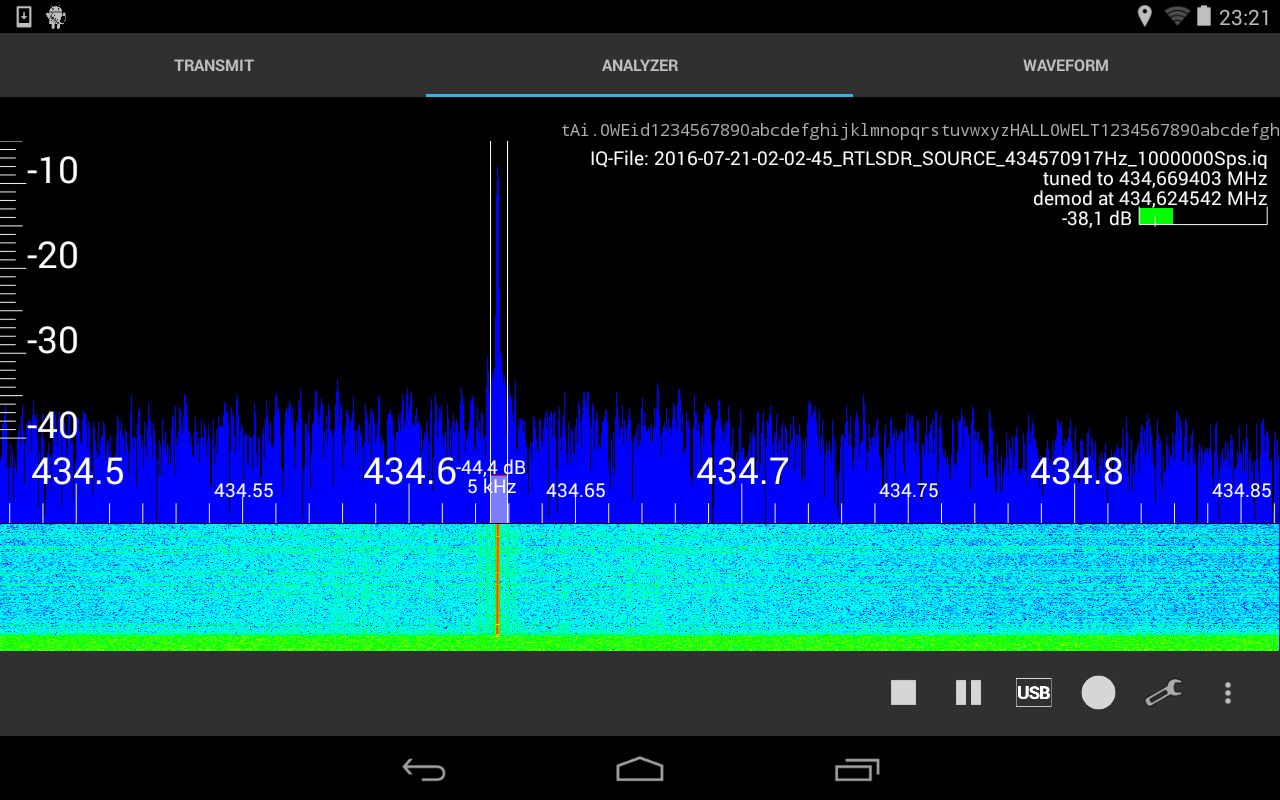
\includegraphics[width=1\linewidth]{gfx/psk31/psk31_android_screenshot.png}
	\caption{Screenshot of the PSK31 demodulator on a Nexus 7}
	\label{fig:psk31_android_screenshot}
\end{figure}

\subsection{Logging\label{sec:logging}}

As explained in \autoref{sec:demod_design}, digital demodulators use the EventBus library to pass demodulated text and other information to the user interface. In order to not only display but also persist this data, the class \texttt{Logger} listens to \texttt{DemodInfoEvent}s from the modulators and, if logging is enabled in the preferences by the user, writes them to logfiles.

\texttt{DemodInfoEvent} has an attribute \texttt{position}, which can be either \texttt{TOP} or \texttt{BOTTOM}, depending on whether the contained text is to be displayed on the upper or the lower line of \texttt{DemodulationInfoView}. Accordingly, the \texttt{Logger} maintains one logfile for the upper and the lower line. Every \texttt{DemodInfoEvent} is logged to one of these files depending on their \texttt{position} attribute. The paths of the logfiles can be defined in the \textsc{Demod} preferences.


\section{Support for new SDR Platforms}

\ac{AnSiAn} supports different \ac{SDR} hardware such as:
\begin{itemize}
	\item RTL-SDR dongle
	\item HackRF
\end{itemize}

The architecture of the app allows to easily add support for additional hardware,
as long as it provides IQ data samples and an Android driver is available.

\subsection{rad1o}

The \emph{rad1o} is a \ac{SDR} platform with the same design as the
\emph{HackRF} that was used as badge for the \emph{Chaos Communication Camp}
2015. Some modifications to the design were made in order to reduce costs and
therefore, minor differences exist compared to a HackRF (e.g. the option to
activate the antenna power is missing for the \emph{rad1o}).

The \emph{rad1o} offers the same USB interface as the \emph{HackRF} and can be
used with the same driver, which is \emph{hackrf\_android}. The driver only needs
two minor modifications:
\begin{enumerate}
	\item If the driver detects a \emph{rad1o}, the option to enable the antenna power
		is disabled.
	\item Because the \emph{rad1o} has a different USB product ID, the driver has
		to be extended in order to also detect a \emph{rad1o} as valid \emph{HackRF}.
\end{enumerate}

Both changes have been applied to the \emph{hackrf\_android} driver. Unfortunately, the
creators of \ac{AnSiAn} have replaced the driver library with a plain copy of the driver
source code, which makes it hard to update it to a newer version. Therefore, the
driver code was removed from \ac{AnSiAn} and replaced again with the current version
of the driver library.

This is the only change necessary to add support for the new \ac{SDR} hardware. 
The \emph{rad1o} can now be used by selecting the \emph{HackRF} source in \ac{AnSiAn}.


\subsection{SDRPlay}

The \emph{SDRplay} is a low cost \ac{SDR} with a frequency range between 100 kHz and
2 GHz. It has a 12-bit \ac{ADC} and therefore suffers less from quantification noise
than the \emph{HackRF} and the \emph{RTL-SDR} (both having an 8-bit \ac{ADC}).
Additionally, it provides passive \ac{RF} filters on the front end to prevent strong
out-of-band noise from distorting the input signal.

Martin Marinov developed an Android driver for the \emph{SDRplay} dongle, which
is currently in beta state. The API is similar to the \emph{RTL-SDR} driver which is
developed by the same person.

\subsubsection{Implementation}

The \emph{SDRplay} driver is started by an Intend with an URL of the format
\texttt{'iqsrc://\ldots'}. It takes an IP address and TCP port as arguments and
will open a socket respectively. The host app can then connect to the socket and
will receive the samples via TCP. Control commands such as changing the
frequency, sample rate or other parameters can be sent through the TCP socket
to the driver. A list of supported commands can be found on the GitHub page
of the driver. They are listed in \autoref{tab:sdrplay_cmds} in the appendix.


\subsubsection{Open Issues}

As the \emph{SDRplay} Android driver is still in beta stage, the support in AnSiAn has
also still beta status. 12-bit samples are currently not working correctly and
therefore \ac{AnSiAn} uses the RTL-SDR compatibility mode of the driver which
delivers stripped 8-bit samples. However, the 12-bit converter code is ready to
be used and might be enabled in future versions of \ac{AnSiAn}.


\section{Transmission\label{sec:transmission}}

RF Analyzer as well as \ac{AnSiAn} both have a receive-only signal processing chain, even though they support \ac{SDR} devices which are capable of transmitting signals, such as the \emph{HackRF}. This section covers the design and (partial) implementation of a transmission chain to make use of supported devices' transmission capabilities.


\subsection{Design}

The implementation of a complete transmission chain is split into multiple steps
to go along with the Agile approach (see \autoref{fig:tx_chain}).

\begin{figure}
\subfloat[Step 1: Raw IQ File Transmission]{%
  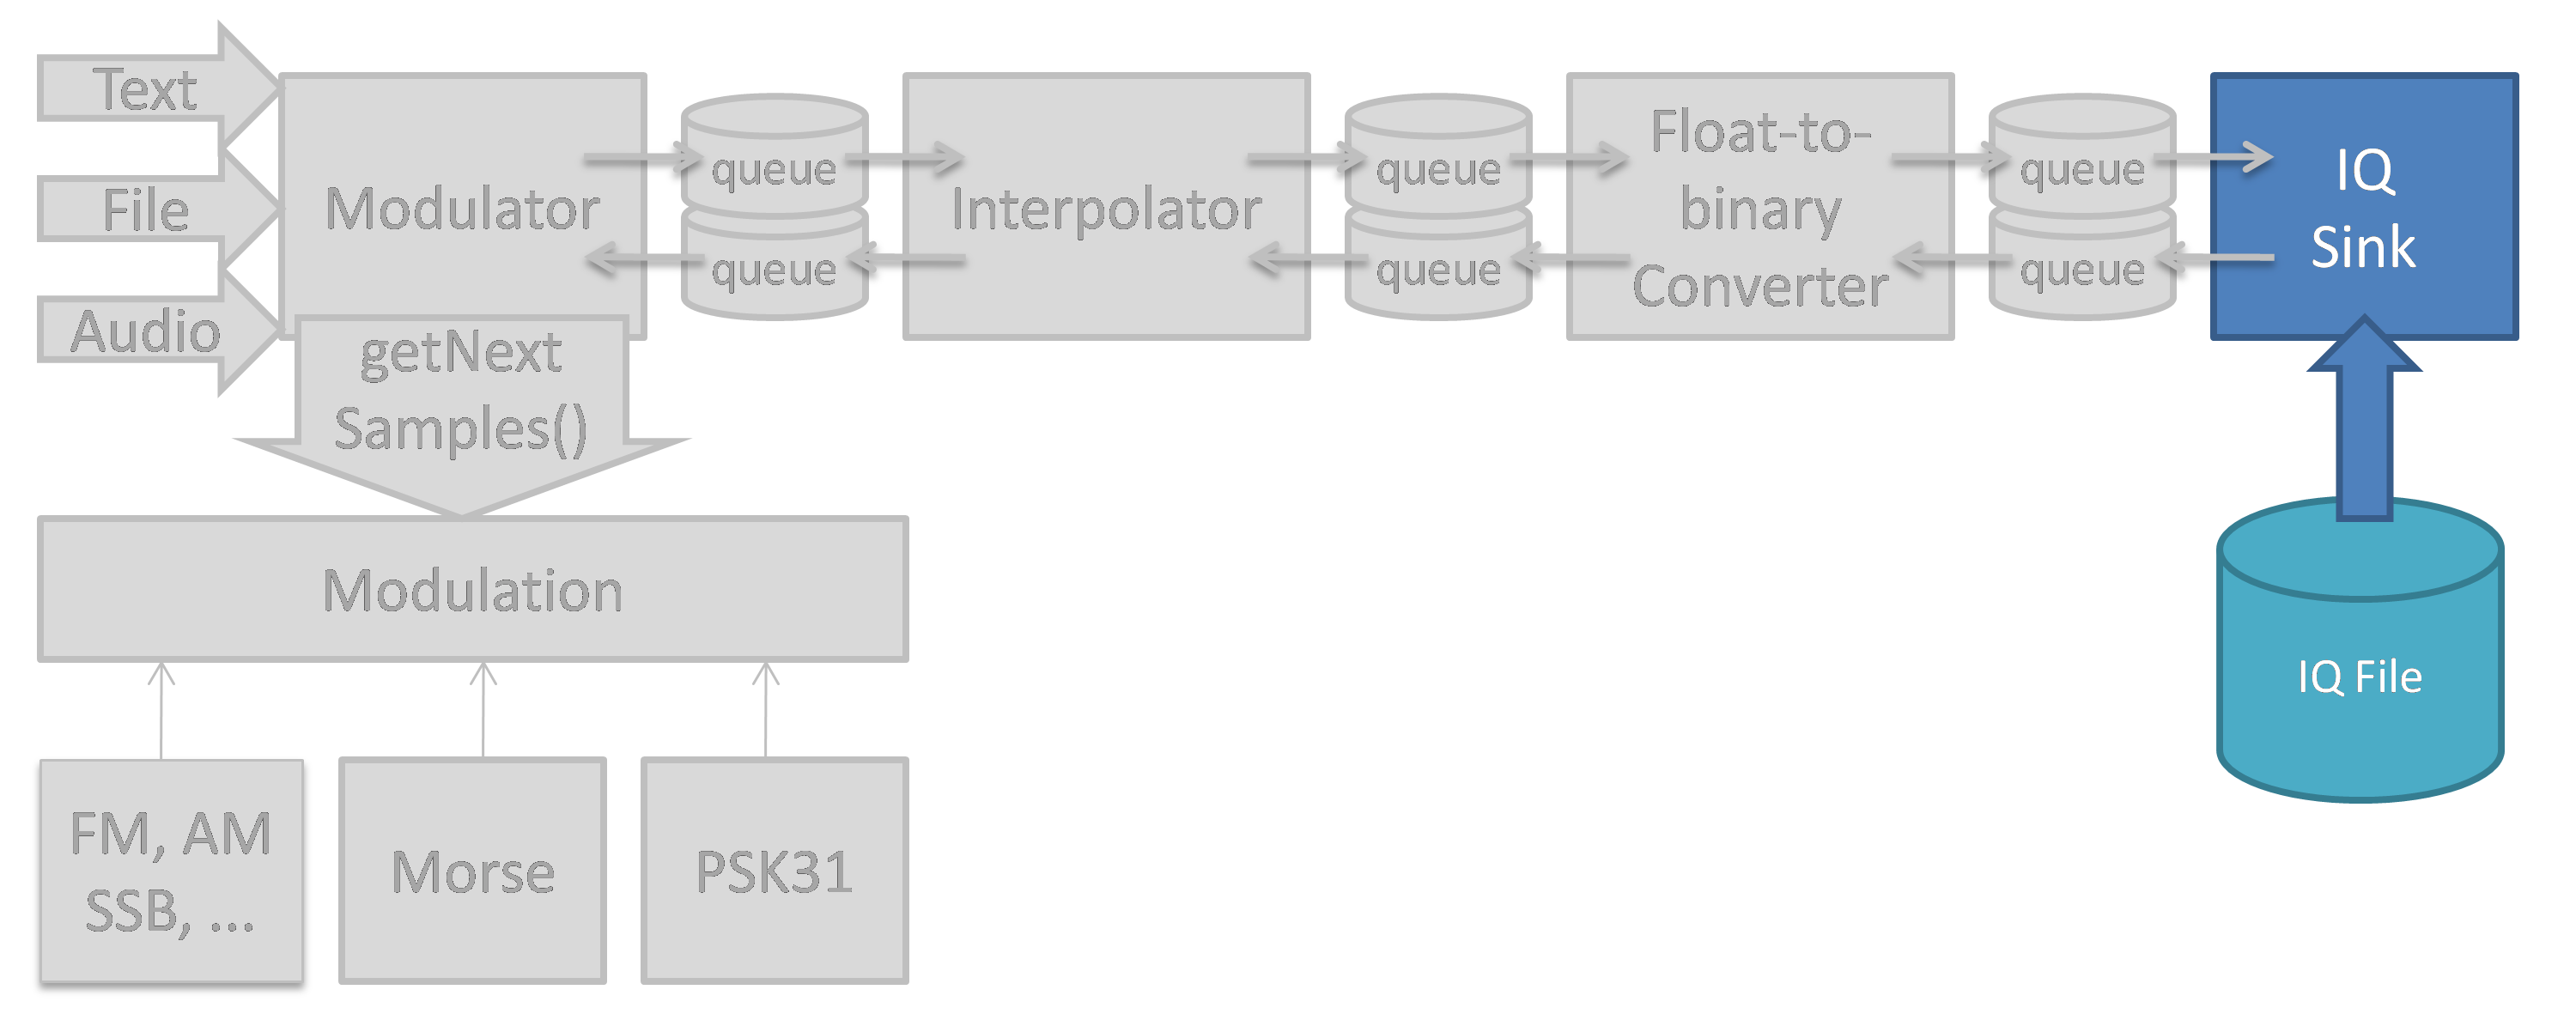
\includegraphics[clip,width=1\linewidth]{gfx/TX_chain_step1.png}%
}

\subfloat[Step 2: Modulated data is written to an IQ file and send afterwards]{%
  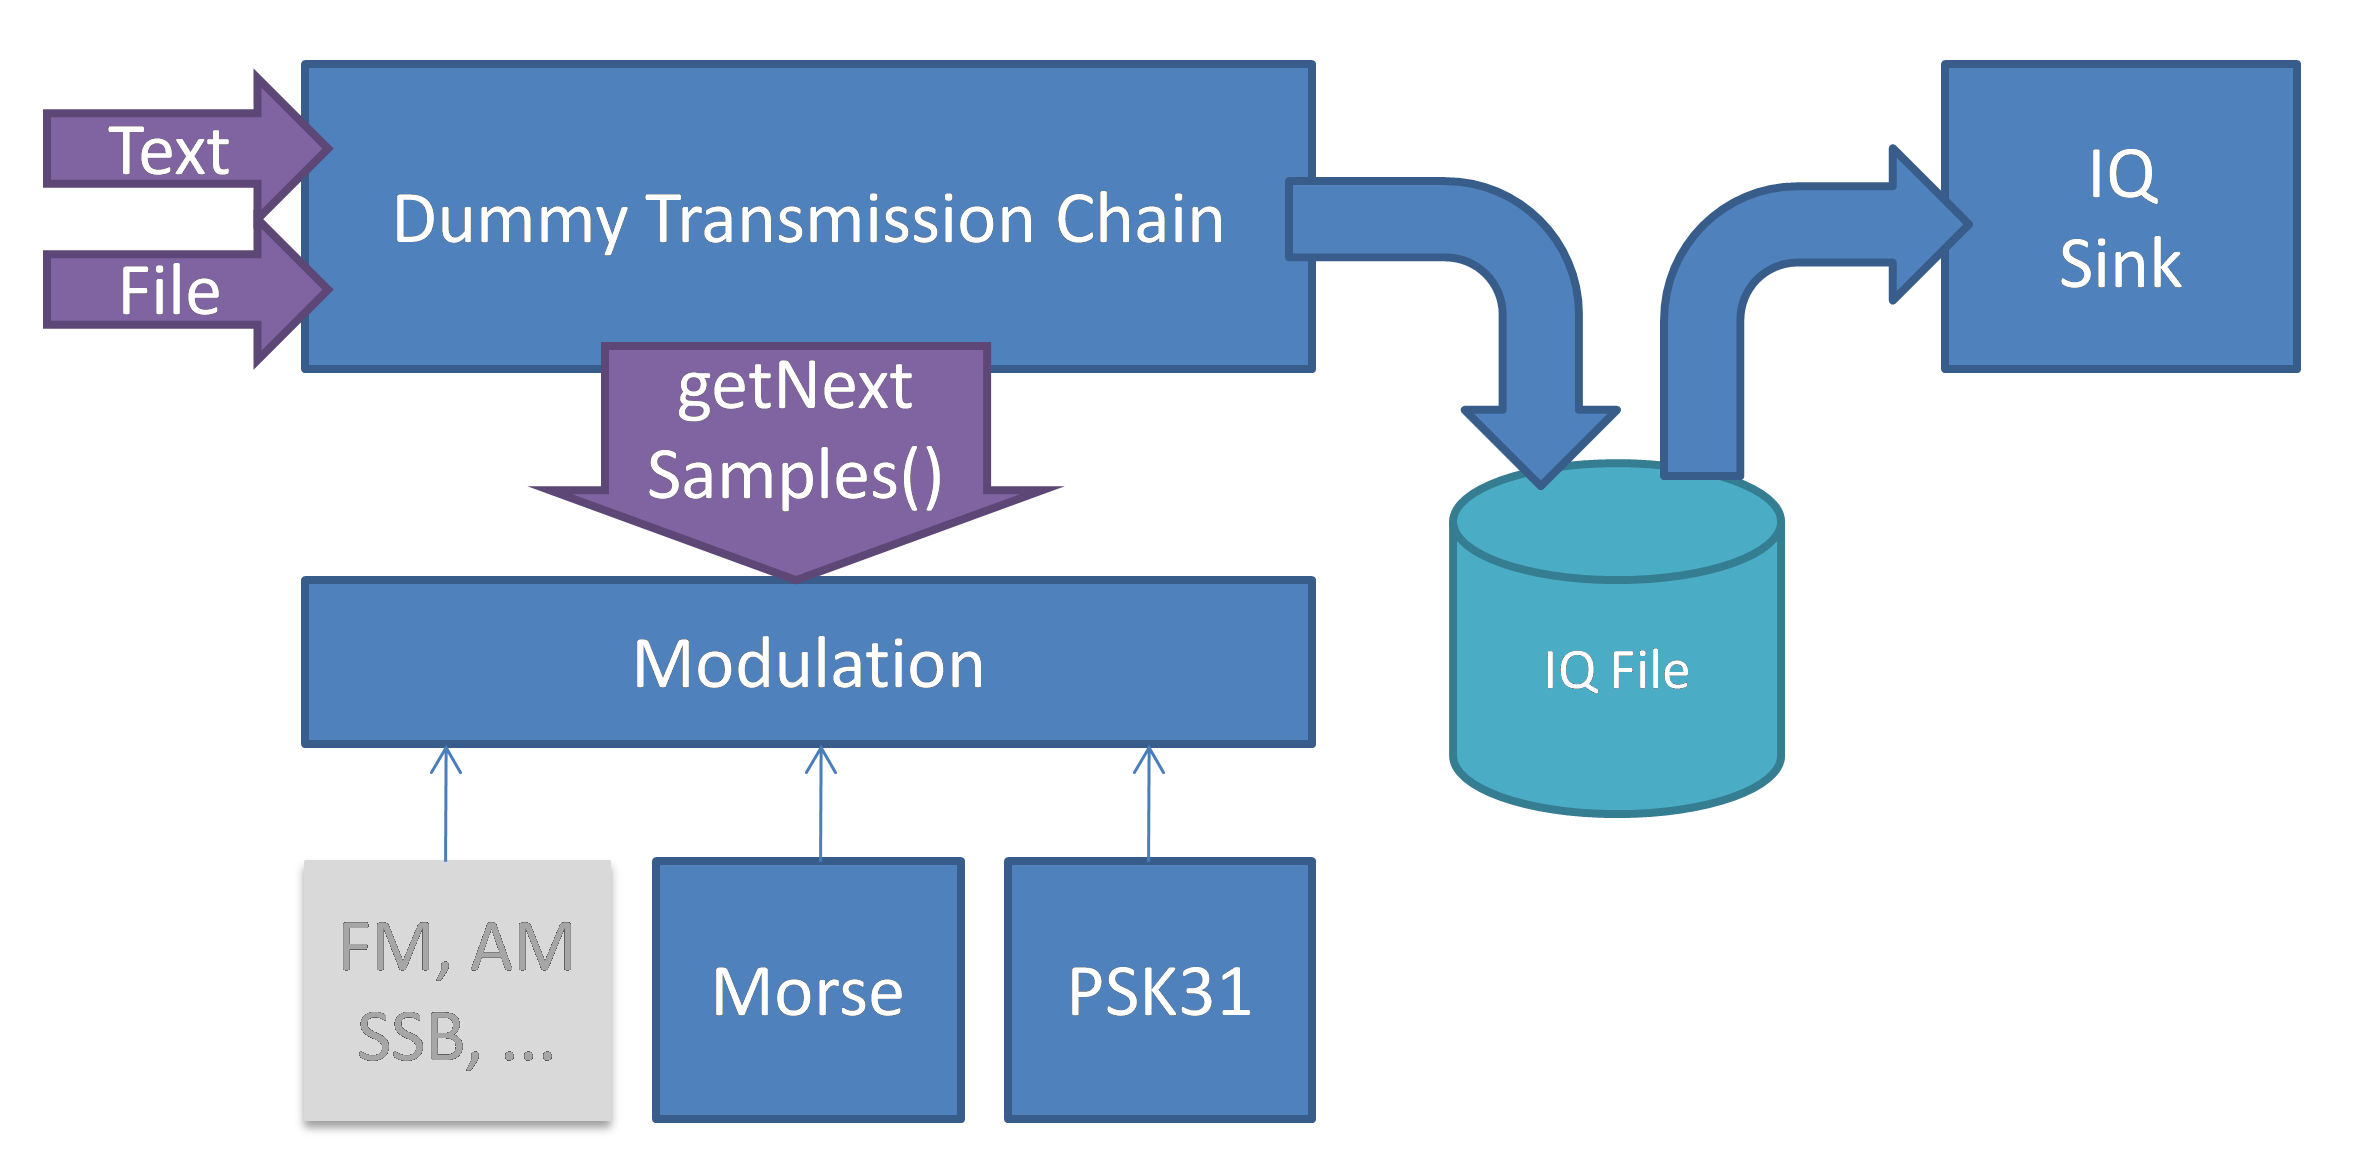
\includegraphics[clip,width=1\linewidth]{gfx/TX_chain_step2.png}%
}

\subfloat[Step 3: Real-time modulation, interpolation, conversion and transmission]{%
  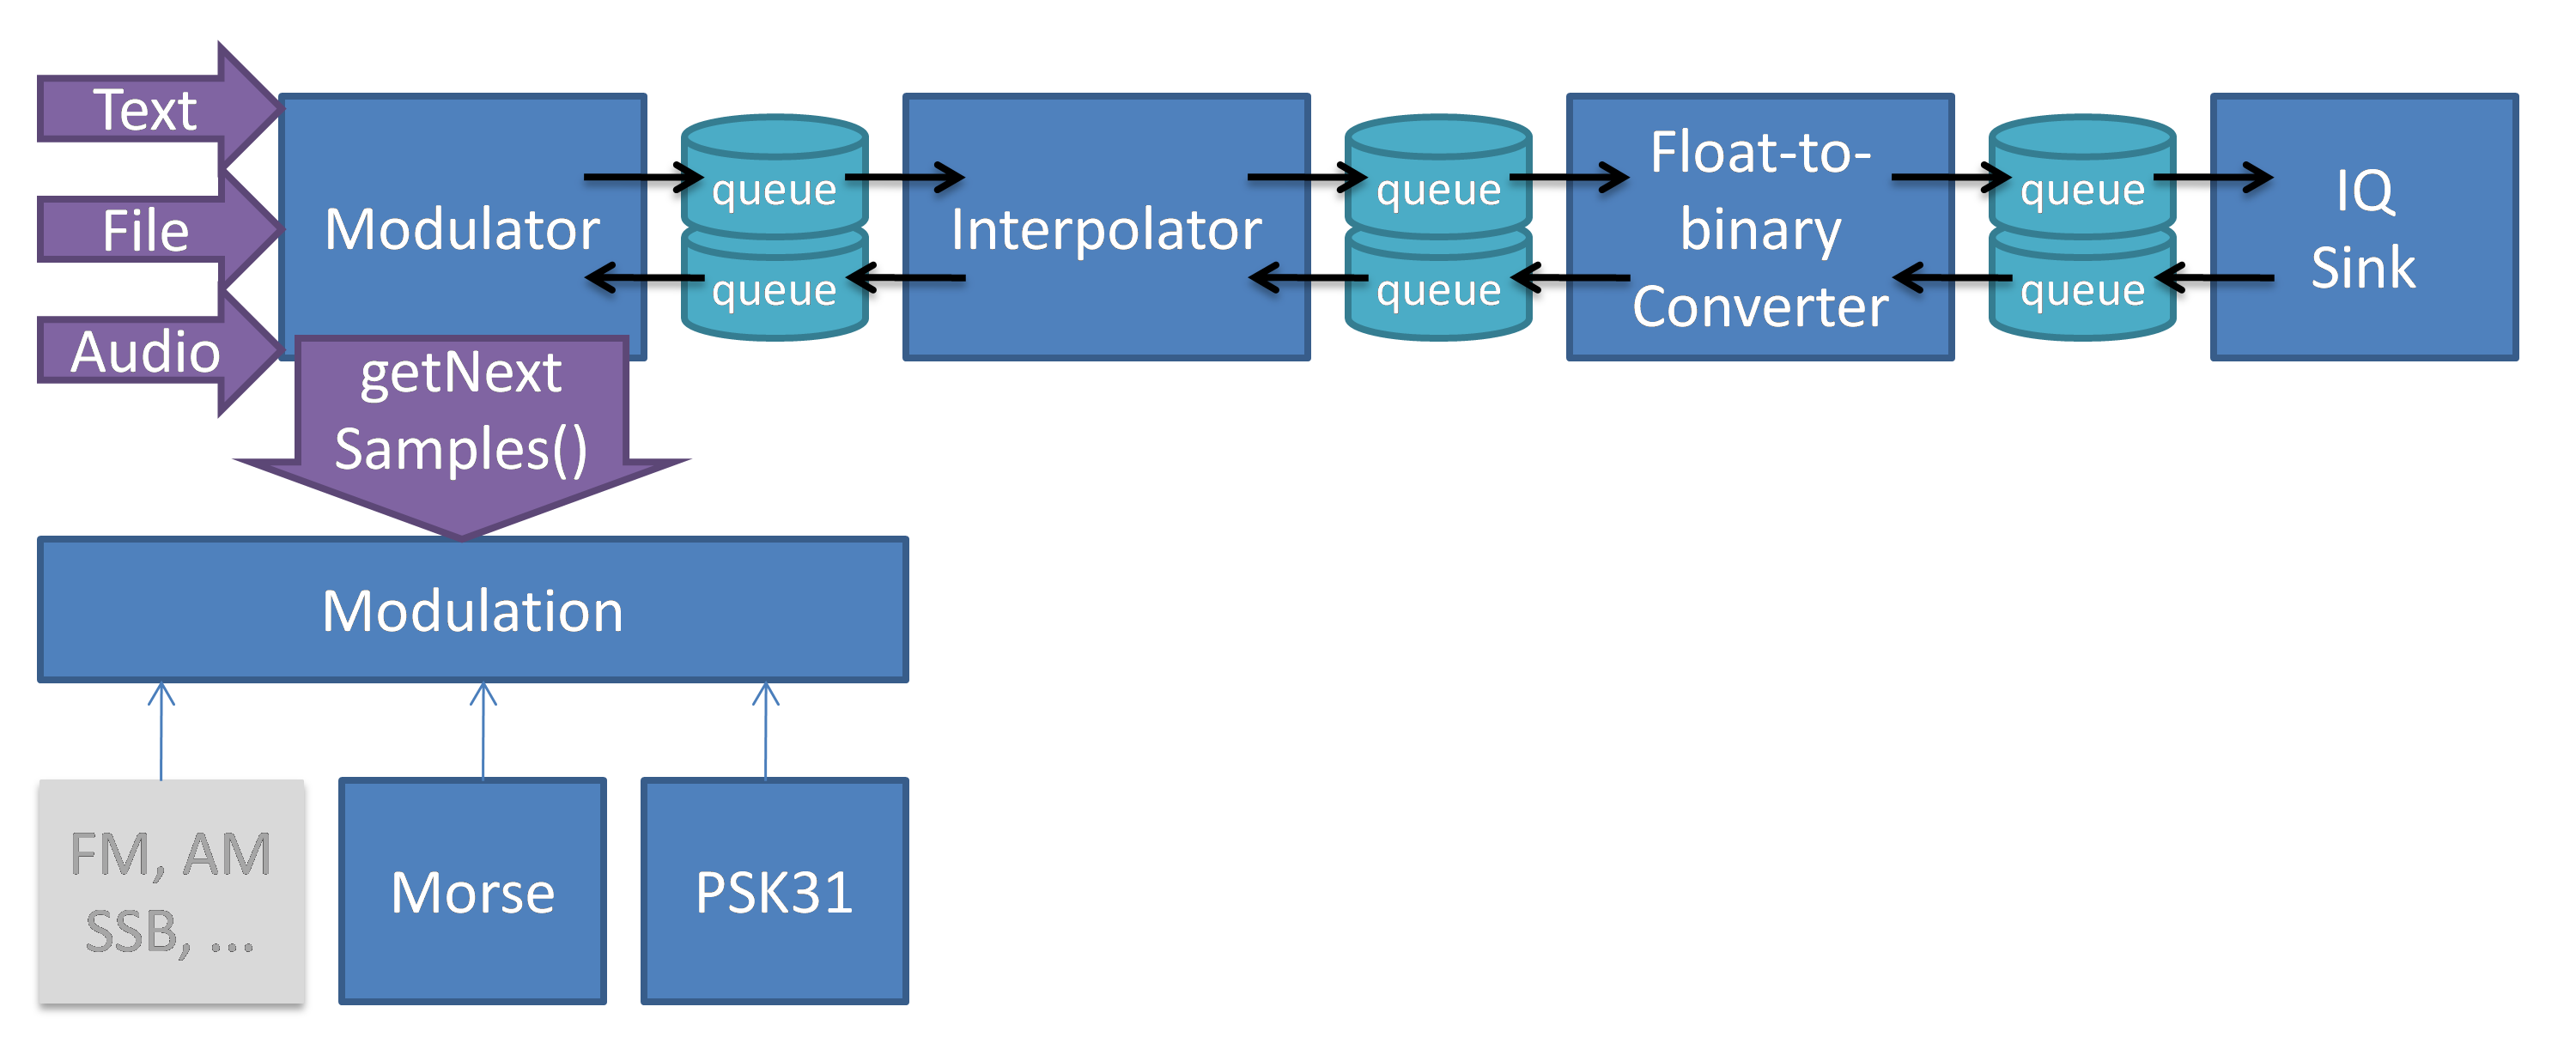
\includegraphics[clip,width=1\linewidth]{gfx/TX_chain_final.png}%
}
\caption{Incremental implementation steps of the transmission chain}
\label{fig:tx_chain}
\end{figure}

In the first step the transmission chain will only include the \texttt{IQSink} which is
able to replay a recorded IQ file. The file has to have the correct format according
to the \ac{SDR} hardware and the sample rate cannot be adjusted.

The second step will provide \texttt{Modulators} for some digital and analog modes along
with a dummy transmission chain which will use the modulator to create an IQ
file and feed it to the \texttt{IQSink} directly.

In the final step the dummy chain is replaced by the complete transmission chain
which includes:
\begin{itemize}
	\item the \texttt{Modulators} from step two
	\item the \texttt{Interpolator} which is able to adjust the sample rate at the 
		output of the \texttt{Modulators} to a value that is supported by the \texttt{IQSink}
	\item a \texttt{float-to-binary} converter which will output the samples in the correct
		binary format according to the \ac{SDR} hardware
\end{itemize}

After the final step the transmission chain will be able to modulate and transmit
signals in real-time, assuming the Android device is capable of the necessary
calculations.

Step one and two were implemented during the third sprint and provide a proof-of-concept
implementation to demonstrate the transmission capabilities of the app.
Step three is left for future work on the application as well as the
addition of more modulators.


\subsection{Transmission of Raw I/Q Files}

RF Analyzer and \ac{AnSiAn} both use the open-source \emph{HackRF} driver from Dennis Mantz\cite{HackRF_Driver_GitHub}. This driver was released with a simple demo application that allowed the user to record signals to files and retransmit them. The logic of the \texttt{IQSink} is based on code from the demo application that was adapted to \ac{AnSiAn}'s Architecture and extended to work e.g. with the EventBus library.

For efficiency, the \emph{HackRF} driver uses asynchronous calls and cycling buffers. The calling program gets assigned free buffers from the driver's queue as they become available and fills them with the data that is to be transmitted. Unfortunately, the driver does not offer any possibility to register a callback function that is called when the driver has finished transmitting all queued data.

A drawback of the current implementation of \texttt{IQSink} is that it transmits noise for several hundred milliseconds after the driver has emptied its transmit buffer. This is because the driver apparently takes some time to realize that it sent all data and can stop transmitting. An alternative would be for the program to explicitly tell the driver to stop sending. As the program has no way of knowing when the driver finishes sending, this would either mean stopping the transmission early or having to estimate the remaining transmission time based on the sample rate and queue length. Experiments with the latter did, however, not yield satisfying results.


\subsection{Modulators}

Each \texttt{Modulator} will provide an interface to retrieve the next packet of
modulated samples. The payload data (e.g. audio or text) might be given at
instantiation time or through a queue (in order to enable real-time transmission).

As mentioned above, the step two implementation will include a dummy transmission
chain that reads the output of the \texttt{Modulator}, converts it to binary IQ
data and writes it to a temporary file which will then be transmitted by the
\texttt{IQSink} implemented in the previous section.


\subsubsection{Morse Modulator}

The Morse modulator takes a string as input payload and produces a baseband
signal with dits and dahs respectively. The Morse encoder from the previous
\ac{AnSiAn} version can be reused to transform the payload text into a
sequence of dits ('.'), dahs ('-'), breaks ('\textvisiblespace') and word
boundaries ('/'). Each character in this sequence corresponds to a predefined
packet of IQ samples (see \autoref{tab:morse_modulation}).

Because the dit and dahs each also contains silence of the length of one dit at
the beginning, the letter separator ('\textvisiblespace') and the word separator
('/') need to be one dit length shorter than they actually are.

To increase the modulation performance, the complex sinusoid is generated
ahead of time and the character translation only consists of a copy operation.

\begin{table}
	\begin{center}
		\begin{tabular}{c l}
			Morse element & Corresponding IQ sample structure \\\hline
			. & one dit length of silence + one dit length of tone \\
			- & one dit length of silence + three dit lengths of tone \\
			\textvisiblespace & two dit lengths of silence \\
			/ & six dit lengths of silence \\\hline
		\end{tabular}
		\caption{Translation from Morse elements to IQ samples}
		\label{tab:morse_modulation}
	\end{center}
\end{table}


\subsubsection{PSK31 Modulator}

The \texttt{PSK31} modulator also takes a string as input payload, encodes it with
Varicode and modulates the bits with \ac{BPSK}. The Varicode dictionary of
the PSK31 demodulator can be reused to perform the first step of creating
the bitstream from the payload text. The \ac{BPSK} modulation simply outputs
the samples based on the current state (phase) of the modulator (see
\autoref{tab:bpsk_modulation}).

\begin{table}
	\begin{center}
		\begin{tabular}{c c | c}
			Previous state (phase) & Current bit & BPSK output \\\hline
			0° & 0 & $cos(\frac{\pi \cdot 31.25 Hz \cdot t}{f_s})$ \\
			180° & 0 & $-cos(\frac{\pi \cdot 31.25 Hz \cdot t}{f_s})$ \\
			0° & 1 & 1 \\
			180° & 1 & -1 \\\hline
		\end{tabular}
		\caption{Output of the BPSK modulation based on its previous state}
		\label{tab:bpsk_modulation}
	\end{center}
\end{table}



\section{GUI\label{sec:gui}}

In order to expose the newly implemented features and their parameters to the user, changes to the user interface of \ac{AnSiAn} were necessary. \autoref{sec:prefs} describes the changes made in the preferences menu and \autoref{sec:transmit_tab} covers the \ac{GUI} of the new Transmit Tab. \autoref{sec:freq_dialog} addresses a change in the frequency selection dialog that was made to avoid unexpected behavior.


\subsection{Preferences\label{sec:prefs}}

\begin{figure}
\centering
\subfloat[The old Morse preferences\label{fig:demod_prefs_old}]{
  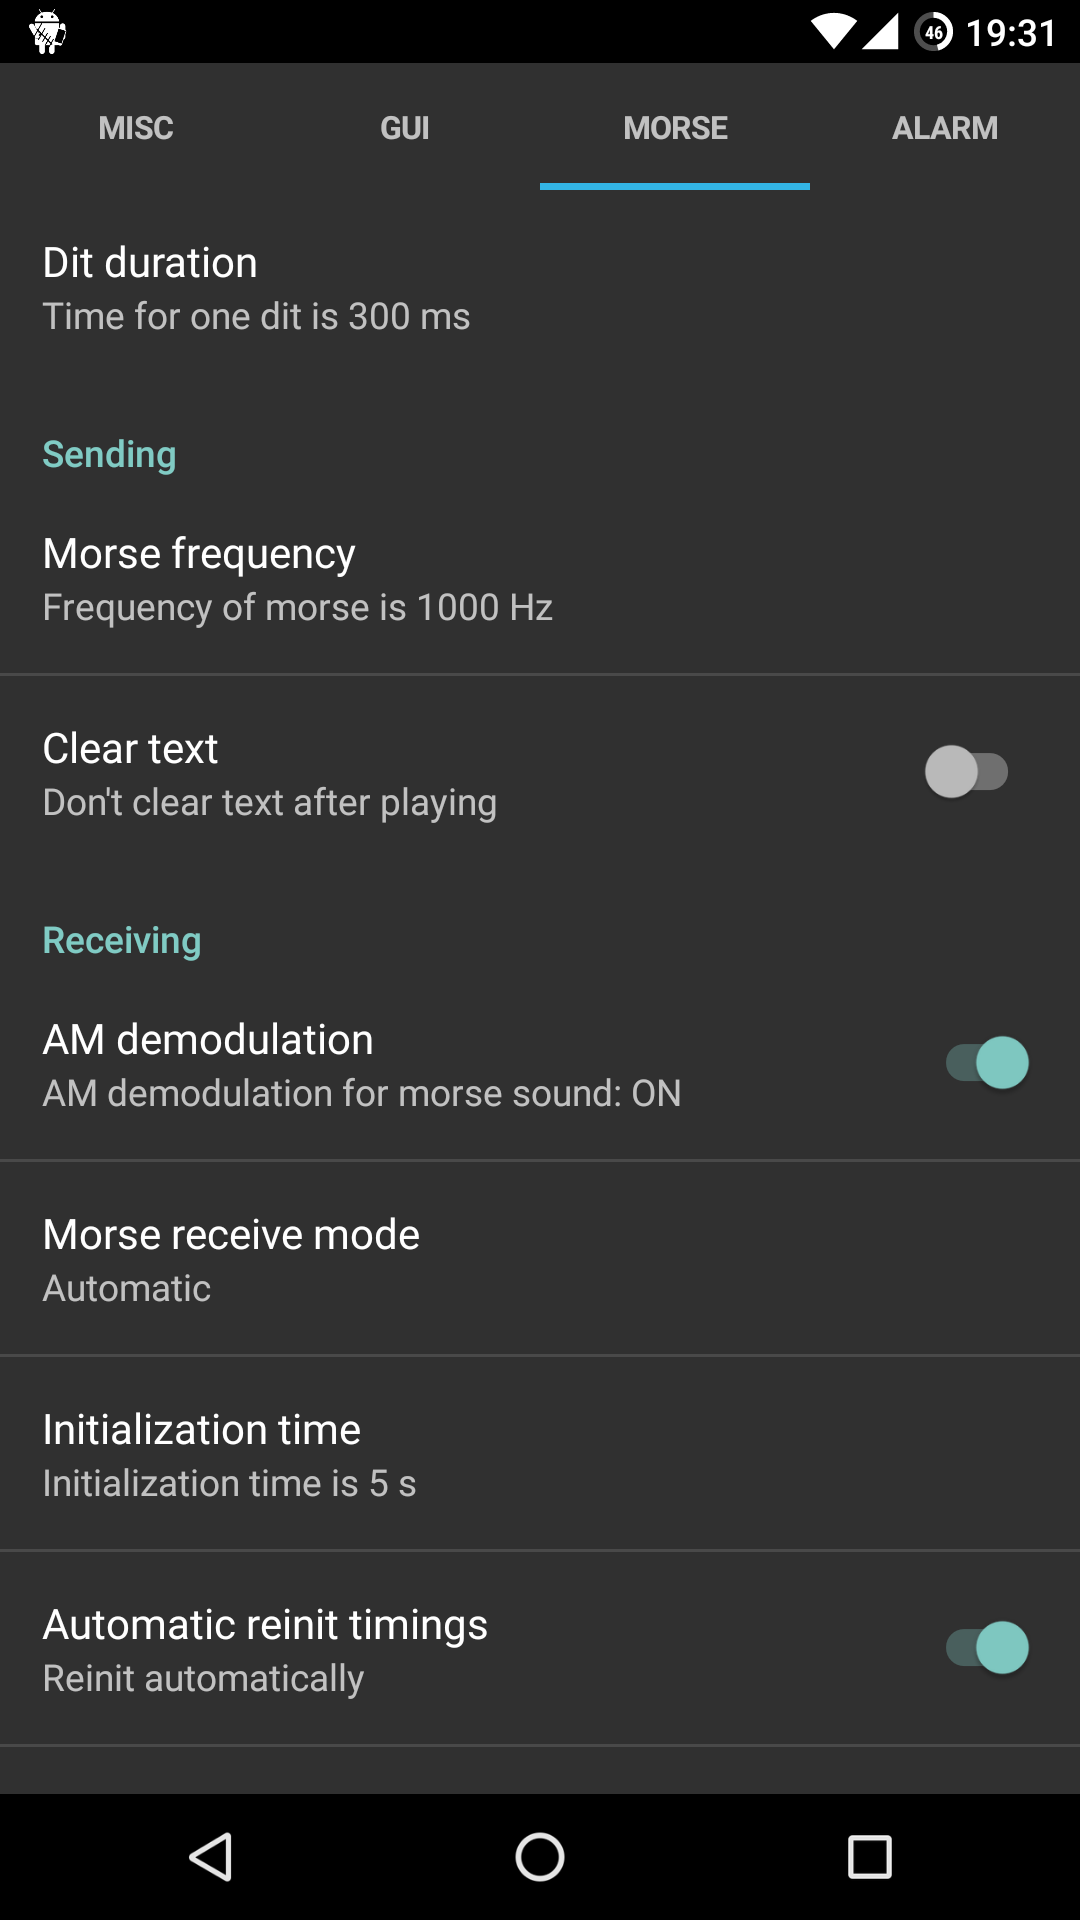
\includegraphics[width=0.4\textwidth]{gfx/screenshots/demod_prefs_old.png}
}
\hfill\null
\subfloat[The new demod preferences]{
  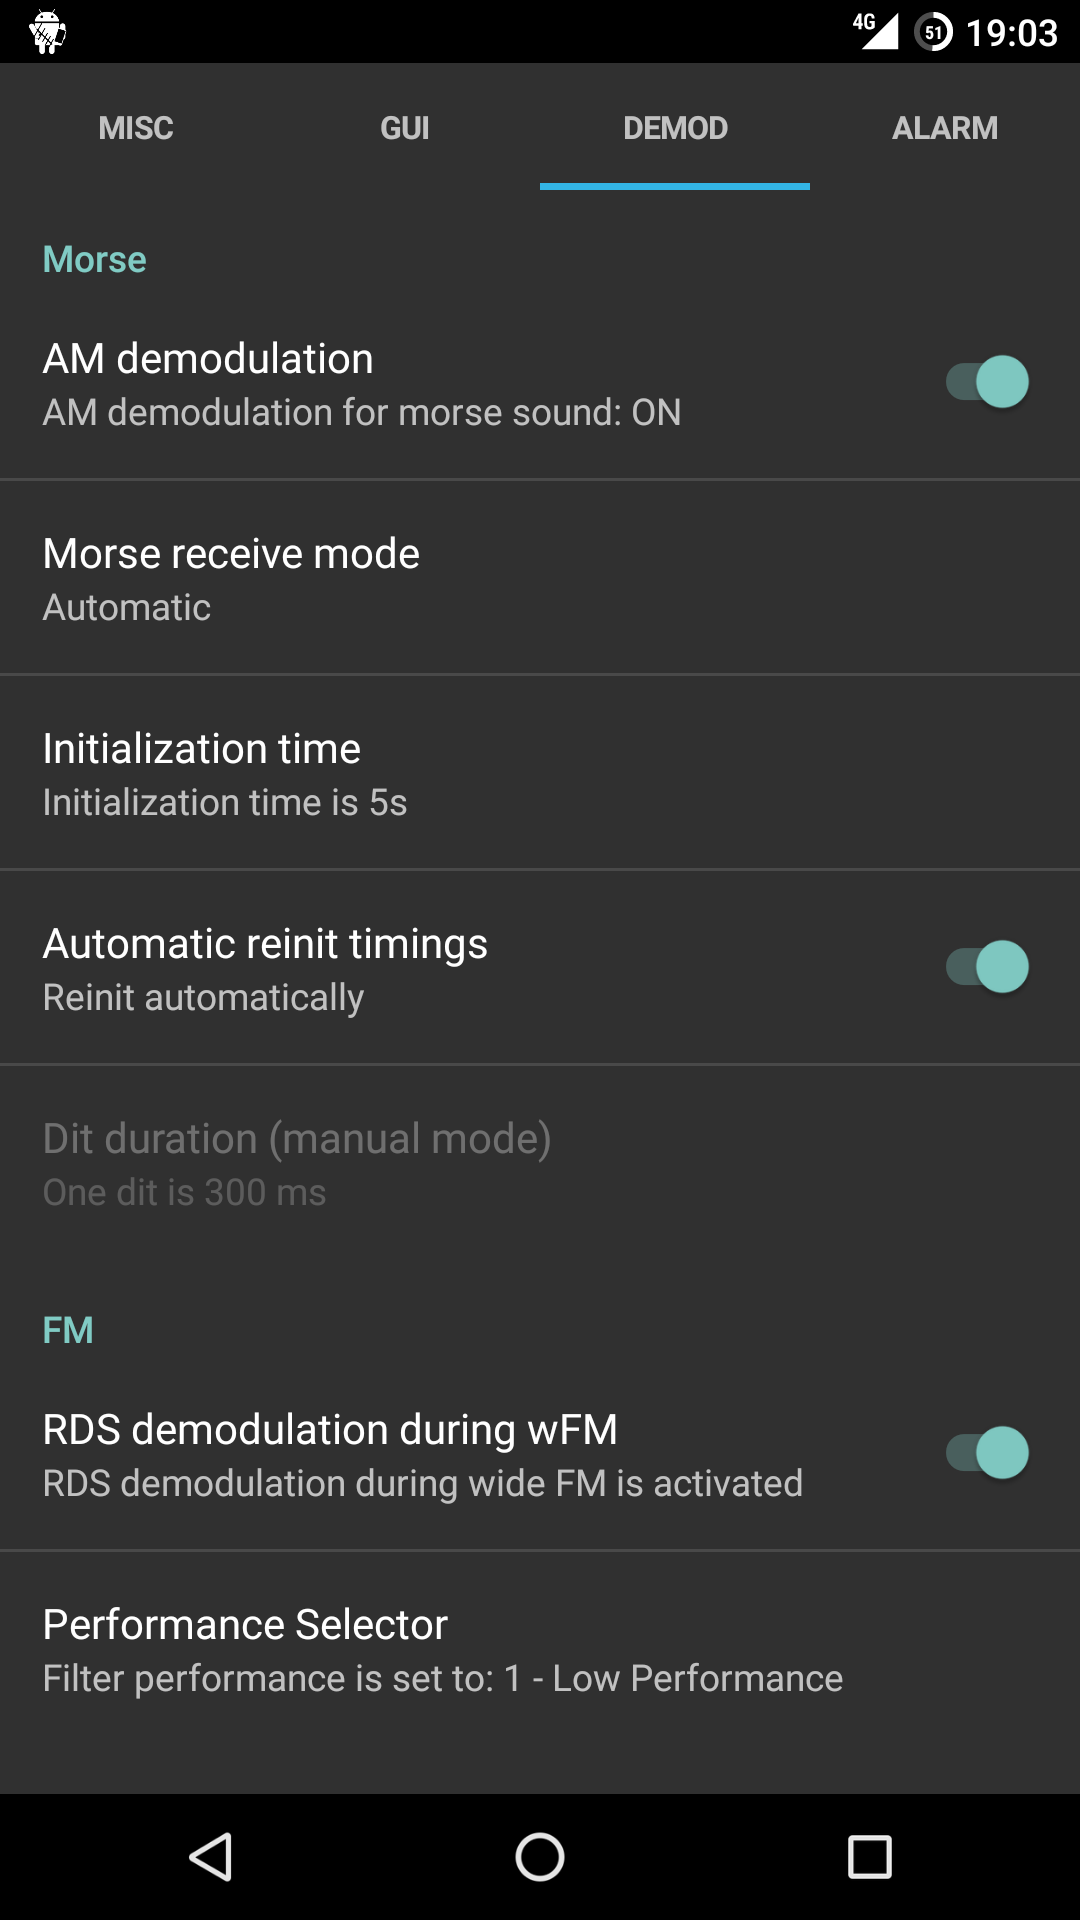
\includegraphics[width=0.4\textwidth]{gfx/screenshots/demod_prefs_new_1.png}
}
\caption{Screenshot of the preference menu on a Nexus 5X}
\label{fig:demod_prefs}
\end{figure}

\ac{AnSiAn} features a preference menu with four tabs that can be seen in \autoref{fig:demod_prefs}. In the original \ac{AnSiAn}, one of these tabs is the Morse tab that holds options for Morse demodulation and audio generation. As the new version of \ac{AnSiAn} replaces Morse audio generation with actual modulation and transmit capability and supports \ac{RDS} and \ac{PSK31} as additional digital demodulation schemes, it was decided to refactor the Morse preference tab into a general \textsc{Demod} preference tab while bundling transmission preferences for all available transmission modes in the \textsc{Transmit} Tab on the main screen (see \autoref{sec:transmit_tab}).

As can be seen in \autoref{fig:demod_prefs}, the \textsc{Demod} preference tab holds preferences for various demodulation modes. It also offers a switch to turn on \ac{PSK31} demodulation on using the \ac{USB} demodulator as well as options to turn on logging of demodulated data and to specify the respective logfiles (both not in the screenshot). 

\subsection{Transmit Tab\label{sec:transmit_tab}}

\begin{figure}
\centering
\subfloat[The old Morse Tab\label{fig:transmit_tab_old}]{
  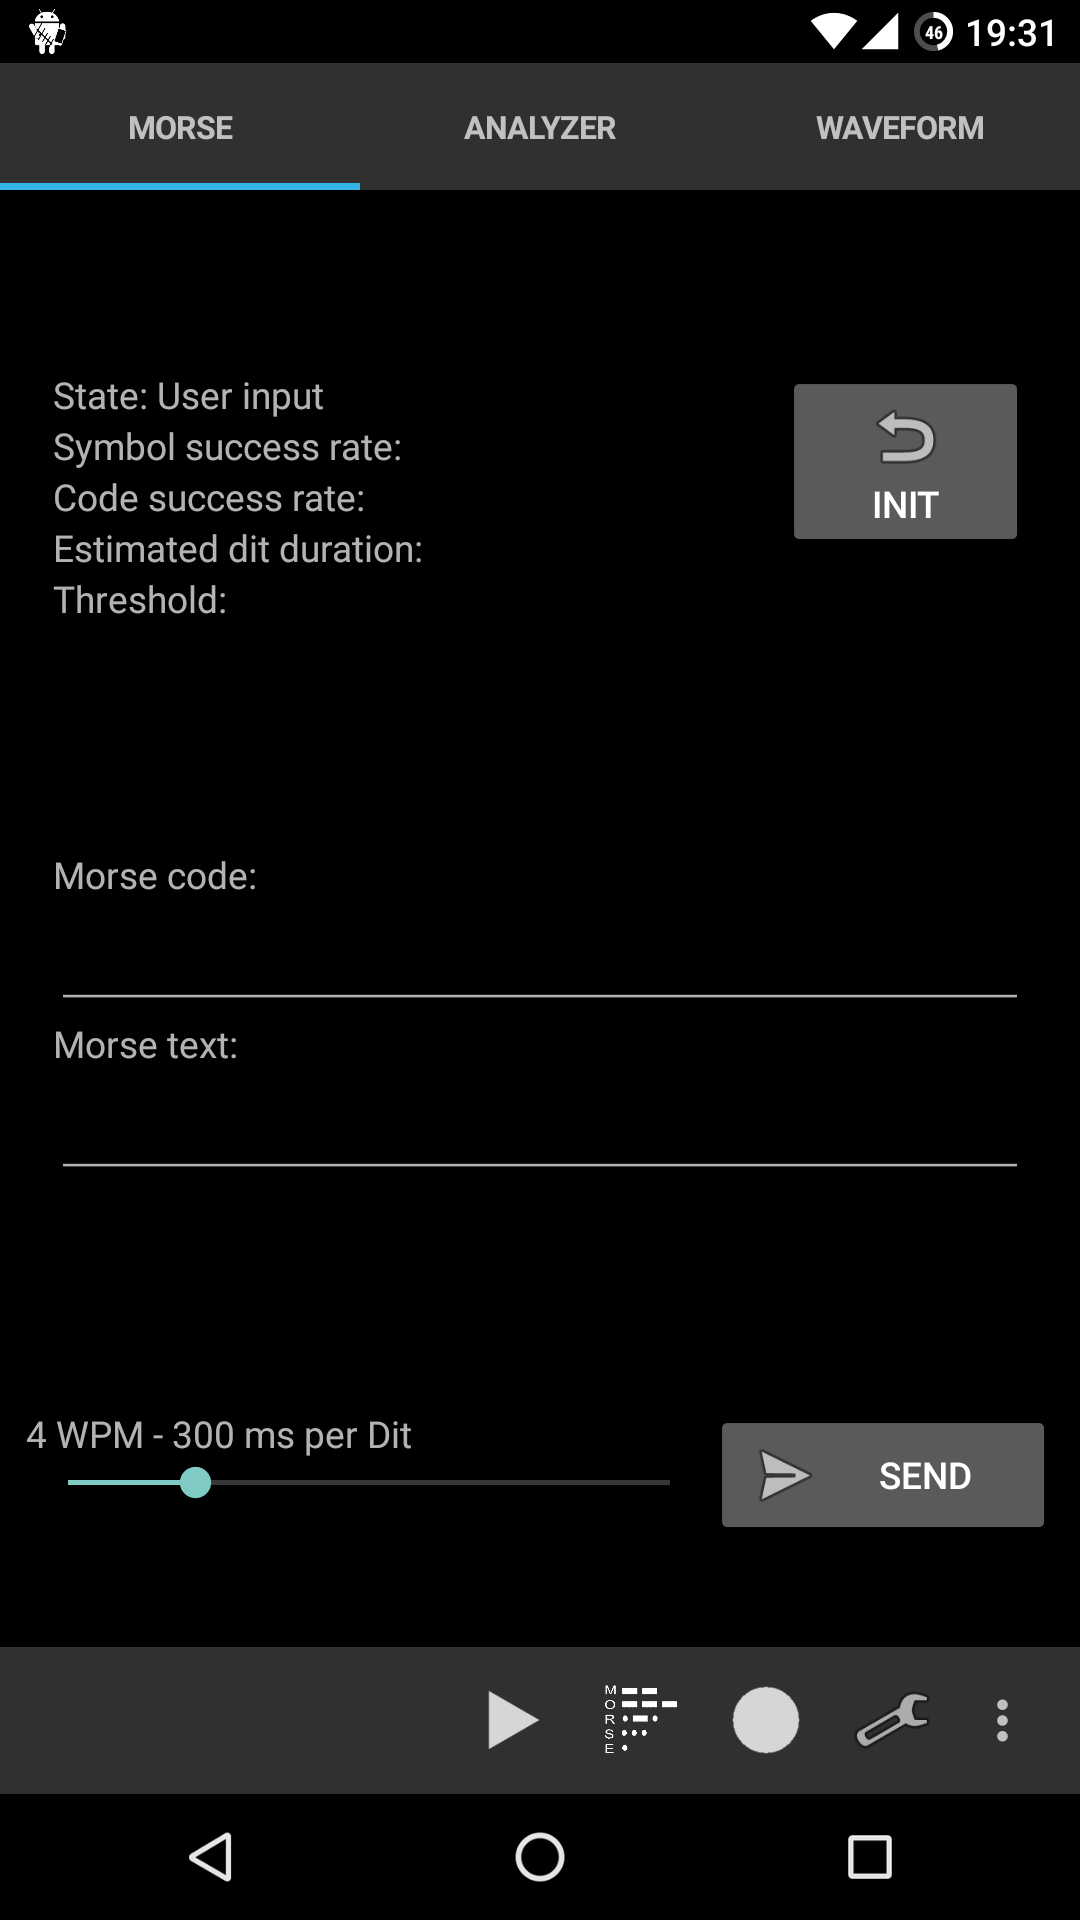
\includegraphics[width=0.4\textwidth]{gfx/screenshots/transmit_tab_old.png}
}
\hfill\null
\subfloat[The new Transmit Tab\label{fig:transmit_tab_new}]{
  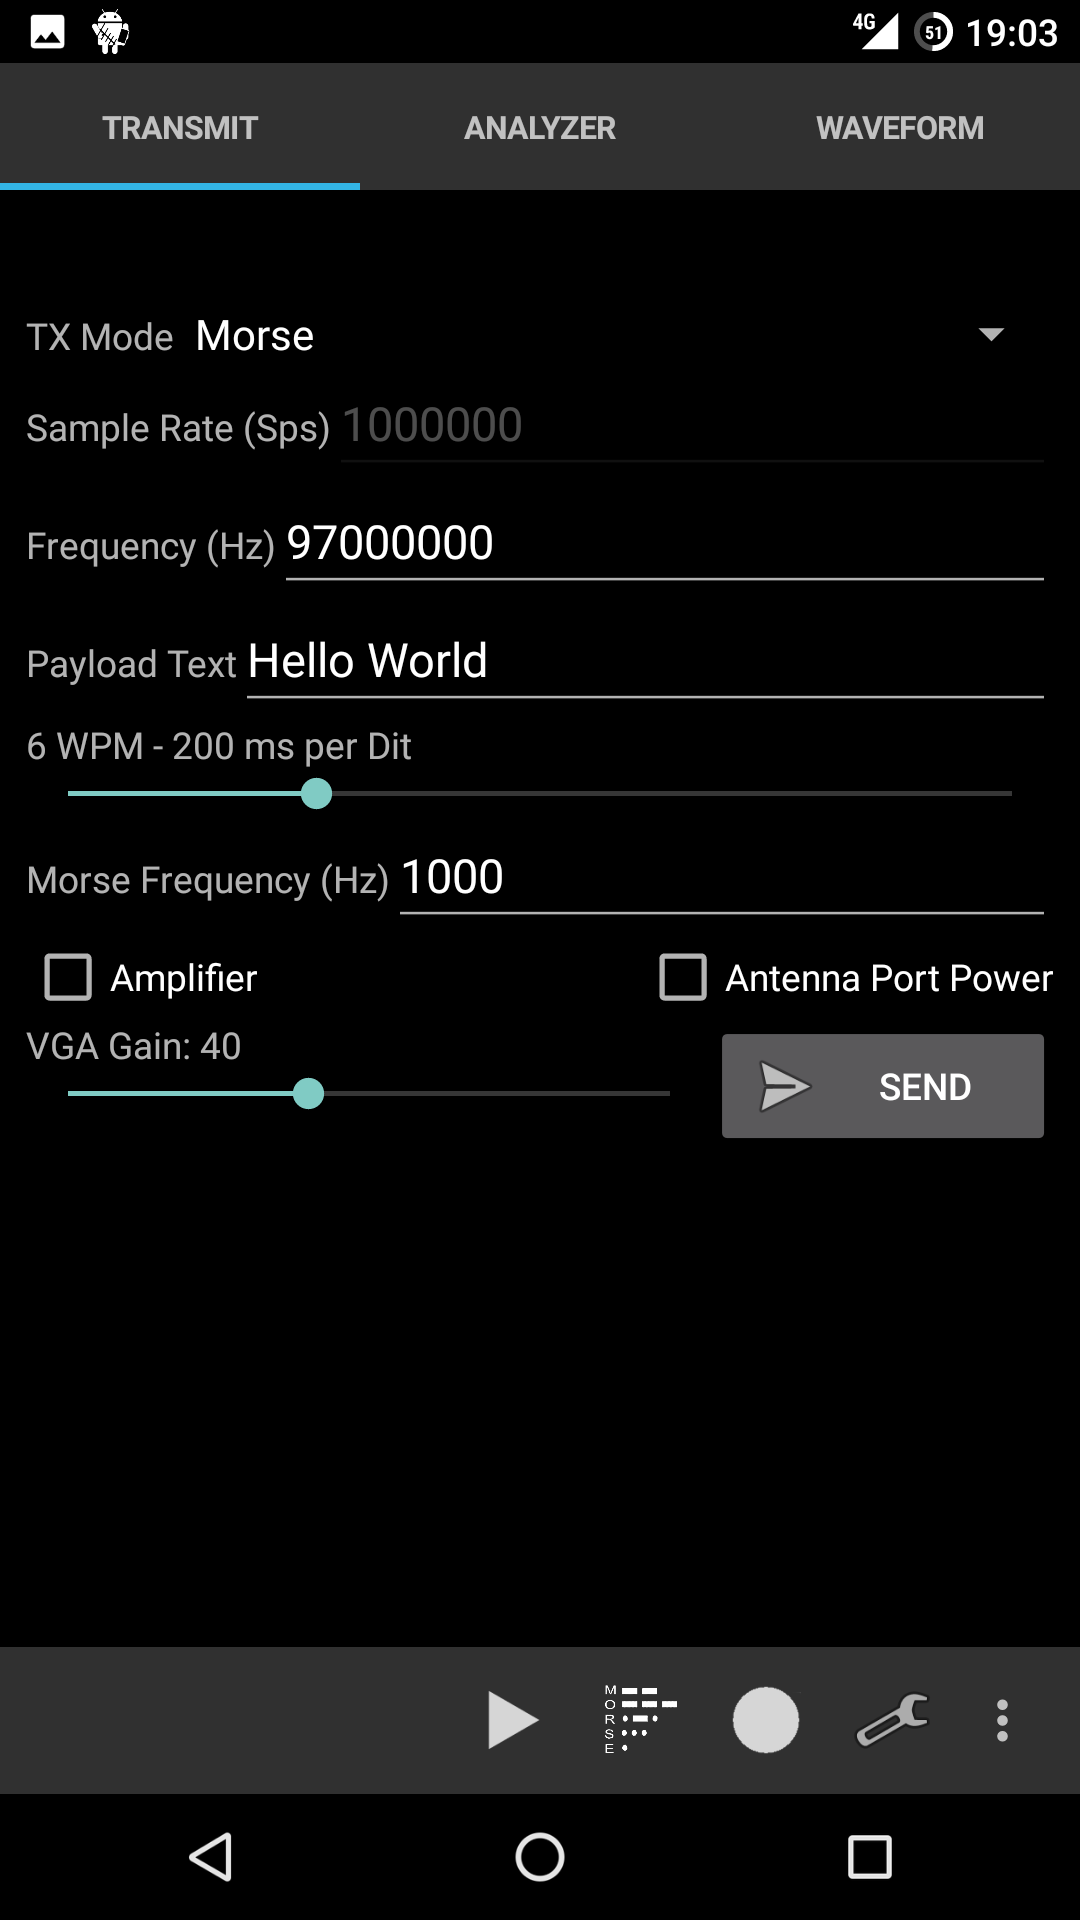
\includegraphics[width=0.4\textwidth]{gfx/screenshots/transmit_tab_new.png}
}
\caption{Screenshot of the Morse/Transmit Tab on a Nexus 5X}
\label{fig:transmit_tab}
\end{figure}

The original \ac{AnSiAn} had a \textsc{Morse} tab that offered information about the state of the Morse demodulator, the possibility to manually re-initialize the demodulator and enabled the user to generate and play Morse audio from text. It can be seen in \autoref{fig:transmit_tab}.

As the newly implemented transmission and modulation feature described in \autoref{sec:transmission} needed a graphical interface, it was decided to refactor the old \textsc{Morse} tab into a \textsc{Transmit} tab that gives the user access to the transmission features. It can be seen in \autoref{fig:transmit_tab} and provides options for the HackRF's features, such as amplification and \ac{VGA} gain. The spinner on the top lets the user select a transmit mode. Available modes are Raw IQ File, Morse and \ac{PSK31}. Fields are hidden, shown or disabled based on the selected mode, i.e. the Morse-specific options for dit duration and Morse frequency are hidden on selecting \ac{PSK31}.


\subsection{Frequency Selection Dialog\label{sec:freq_dialog}}

\begin{figure}
\centering
\subfloat[The old frequency selection dialog]{
  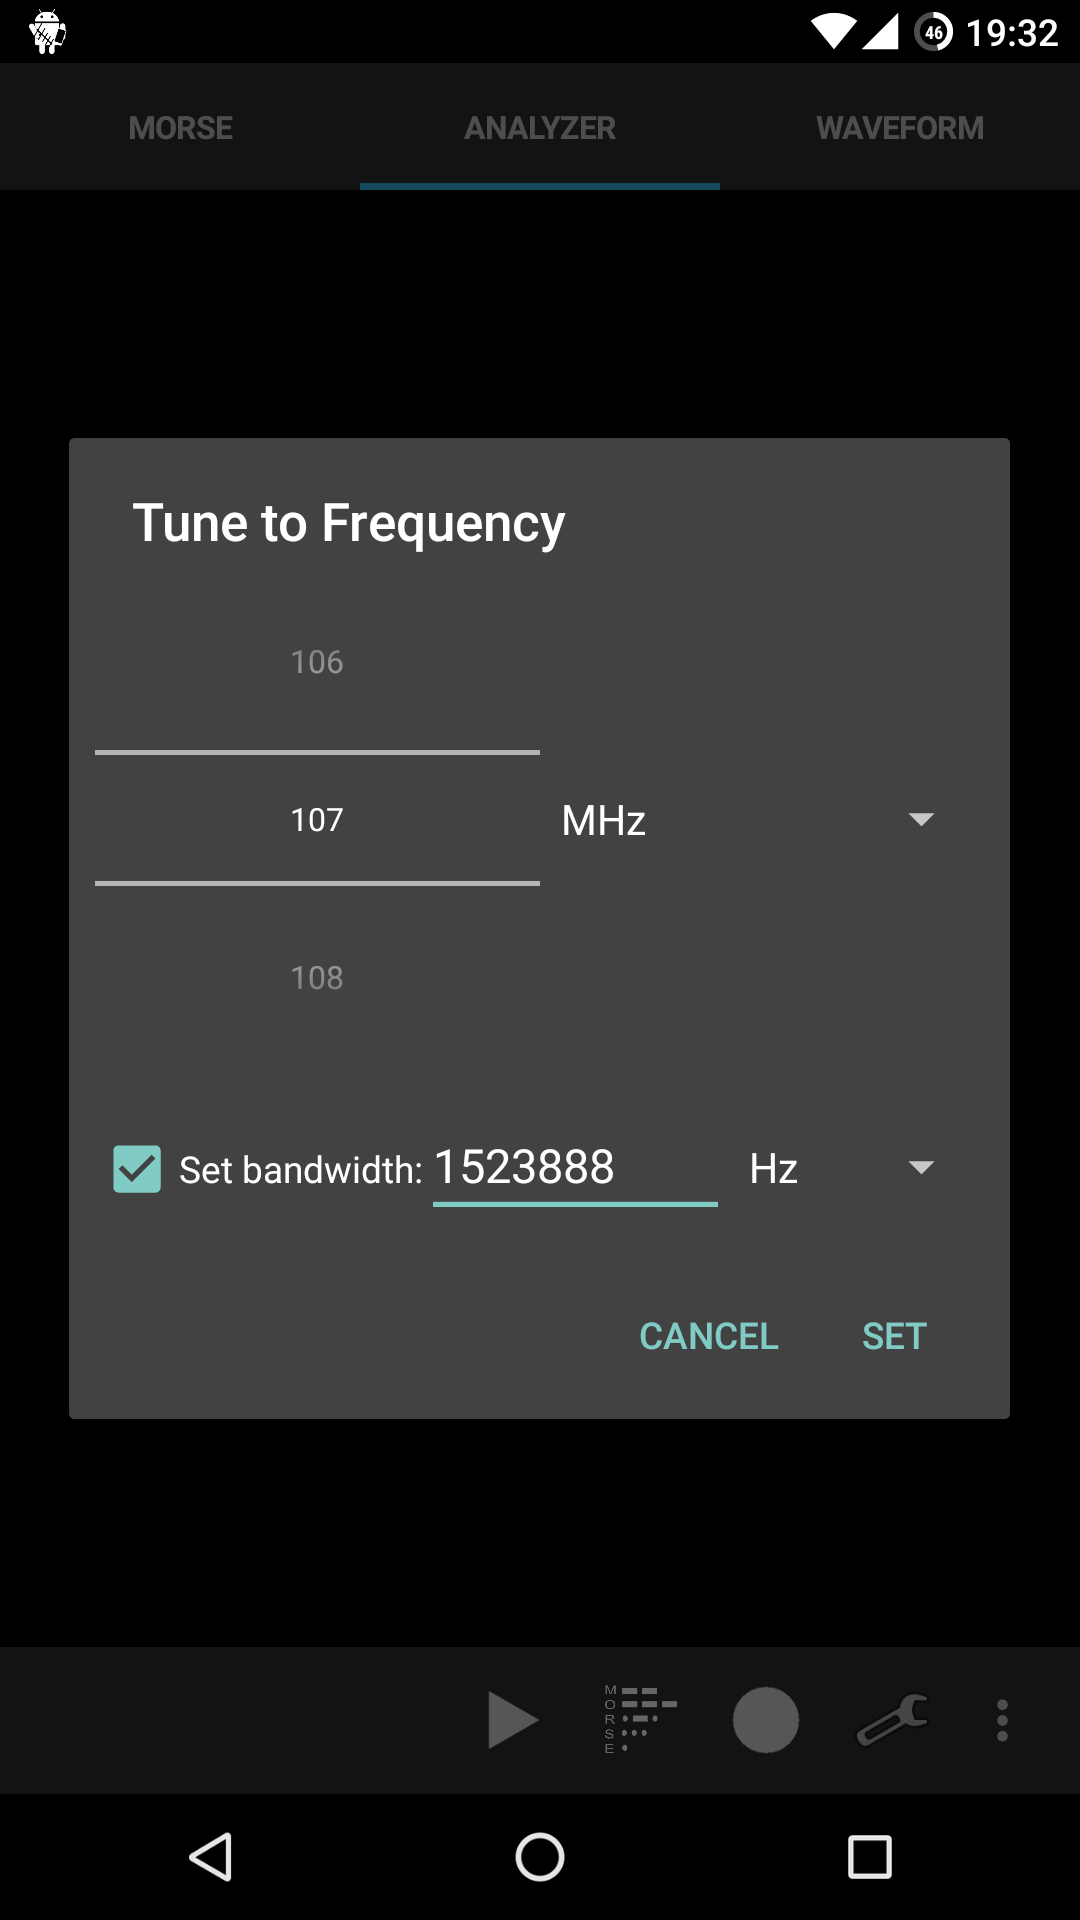
\includegraphics[width=0.4\textwidth]{gfx/screenshots/freq_dialog_old.png}
}
\hfill\null
\subfloat[The new frequency selection dialog]{
  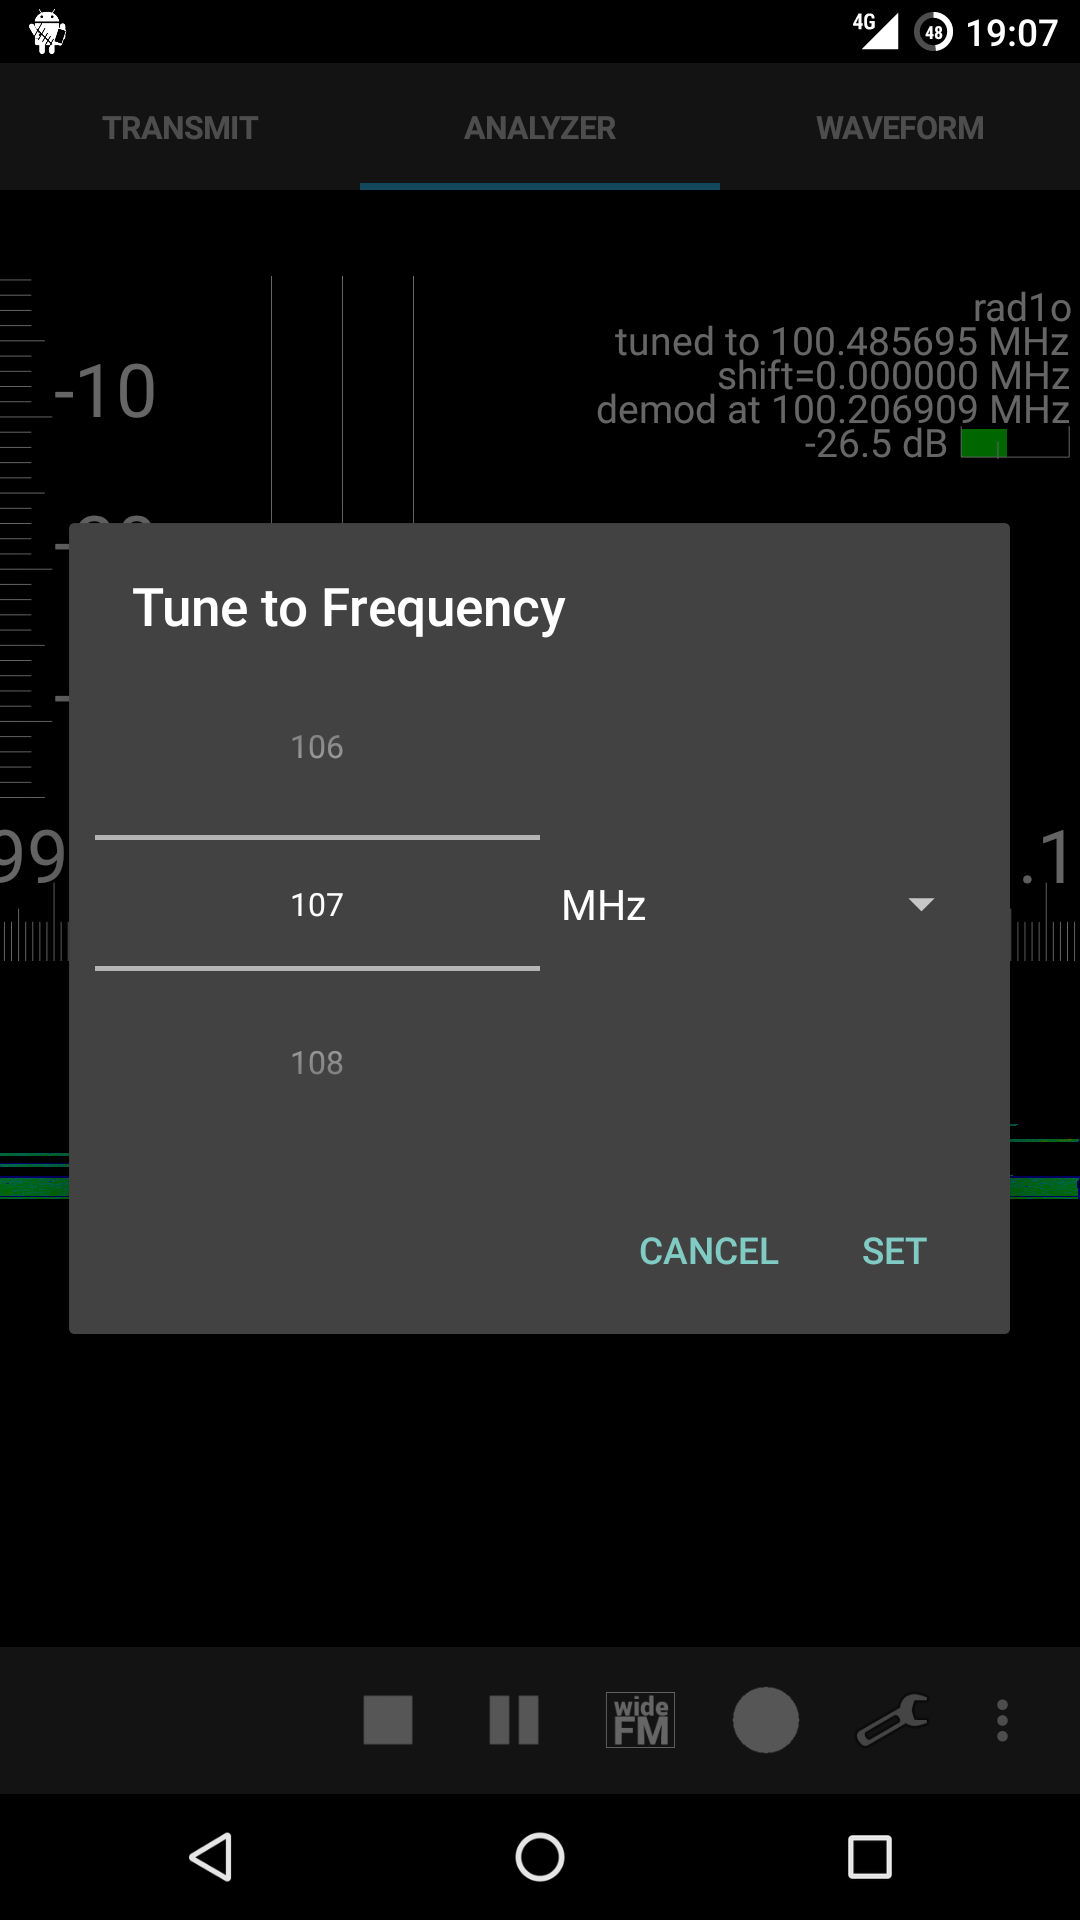
\includegraphics[width=0.4\textwidth]{gfx/screenshots/freq_dialog_new.png}
}
\caption{Screenshot of the frequency selection dialog on a Nexus 5X}
\label{fig:freq_dialog}
\end{figure}

By clicking the menu on the bottom right and then ``Set Frequency'', \ac{AnSiAn} enables the user to quickly tune to a desired frequency without having to scroll through the spectrum. In the original version, this dialog also offers the user to optionally set the sampling rate (called bandwidth in the dialog) to an arbitrary value. By default, this option is enabled and the corresponding field is filled with a value that is not the current sampling rate. A user who only wants to jump to another frequency might therefore inadvertently change the sampling rate.

This has serious consequences, as the demodulation chain can currently only process sampling rates of \SI{1}{\mega{}samples\per\second}. For other sampling rates, the \texttt{Decimator} stops working and does not provide the \texttt{Demodulator} with samples any more. The user does not get any visual feedback on this and can only observe that audio and text demodulation stop working for no apparent reason. As patching the decimator to efficiently support other sampling rates would be a major task, it was decided remove the possibility to change the sample rate in order to prevent users from inadvertently breaking demodulation.

The old and the new frequency selection dialogs can be seen in \autoref{fig:freq_dialog}.

%\include{chapters/perspective}
\chapter{Conclusion\label{ch:conclusion}}

As a fork of RF Analyzer, \ac{AnSiAn} has made huge structural changes to the
application architecture in order to implement a clean \ac{MVC} pattern.
Although this has improved the code quality and maintainability, it also
introduced issues as described in \autoref{sec:cleanup.mem}. These issues and
their impact on other parts of the app (see \autoref{sec:morse_demod}) had to
be addressed before implementing the new features listed in
\autoref{sec:features}. There were also additional features, such as support for
the SDRplay hardware or PSK31 transmission, that were added after the initial
feature list was created and therefore influenced the time schedule.

Nevertheless, all mandatory features, apart from some minor exceptions,
were successfully implemented. This includes new digital demodulation
modes (PSK31 and RDS), logging of demodulator outputs, support for the
rad1o badge and transmission functionality along with some basic transmission
modes (Morse and PSK31) as well as plain I/Q file replay. The \ac{FM}-modulated transmission of audio files and the optional features (Walkie-Talkie-Mode and packet radio demodulation) were not implemented.

Some open tasks and improvements remain to be done in future work on the
application. This includes the implementation of the complete transmission
chain as outlined in \autoref{sec:transmission}, additional modulation modes
and improvements on the \ac{BPSK} demodulation algorithm by switching to
a \ac{PLL}-based approach.


%\part{Appendix}
%%********************************************************************
% Appendix
%*******************************************************
% If problems with the headers: get headings in appendix etc. right
%\markboth{\spacedlowsmallcaps{Appendix}}{\spacedlowsmallcaps{Appendix}}
\chapter{Appendix}\label{ch:Appendix}
\glsresetall % Resets all acronyms to not used

\begin{longtable}{ r l || r l }[h]
	Character & Encoding & Character & Encoding \\\hline
	NUL & 1010101011 				&	!   & 111111111  \\
	SOH & 1011011011 				&	"   & 101011111  \\
	STX & 1011101101 				&	\#  & 111110101  \\
	ETX & 1101110111 				&	\$  & 111011011  \\
	EOT & 1011101011 				&	\%  & 1011010101  \\
	ENQ & 1101011111 				&	\&  & 1010111011  \\
	ACK & 1011101111 				&	'   & 101111111  \\
	BEL & 1011111101 				&	(   & 11111011  \\
	BS  & 1011111111 				&	)   & 11110111  \\
	HT  & 11101111 					&	*   & 101101111  \\
	LF  & 11101 					&	+   & 111011111  \\
	VT  & 1101101111 				&	,   & 1110101  \\
	FF  & 1011011101 				&	-   & 110101  \\
	CR  & 11111 					&	.   & 1010111  \\
	SO  & 1101110101 				&	/   & 110101111  \\
	SI  & 1110101011 				&	0   & 10110111  \\
	DLE & 1011110111 				&	1   & 10111101  \\
	DC1 & 1011110101 				&	2   & 11101101  \\
	DC2 & 1110101101 				&	3   & 11111111  \\
	DC3 & 1110101111 				&	4   & 101110111  \\
	DC4 & 1101011011 				&	5   & 101011011  \\
	NAK & 1101101011 				&	6   & 101101011  \\
	SYN & 1101101101 				&	7   & 110101101  \\
	ETB & 1101010111 				&	8   & 110101011  \\
	CAN & 1101111011 				&	9   & 110110111  \\
	EM  & 1101111101 				&	:   & 11110101  \\
	SUB & 1110110111 				&	;   & 110111101  \\
	ESC & 1101010101 				&	<   & 111101101  \\
	FS  & 1101011101 				&	=   & 1010101  \\
	GS  & 1110111011 				&	>   & 111010111  \\
	RS  & 1011111011 				&	?   & 1010101111  \\
	US  & 1101111111 				&	@   & 1010111101  \\
	SP  & 1 						&	A   & 1111101  \\
	B   & 11101011 					&	c   & 101111  \\
	C   & 10101101 					&	d   & 101101  \\
	D   & 10110101 					&	e   & 11  \\
	E   & 1110111 					&	f   & 111101  \\
	F   & 11011011 					&	g   & 1011011  \\
	G   & 11111101 					&	h   & 101011  \\
	H   & 101010101 				&	i   & 1101  \\
	I   & 1111111 					&	j   & 111101011  \\
	J   & 111111101 				&	k   & 10111111  \\
	K   & 101111101 				&	l   & 11011  \\
	L   & 11010111 					&	m   & 111011  \\
	M   & 10111011 					&	n   & 1111  \\
	N   & 11011101 					&	o   & 111  \\
	O   & 10101011 					&	p   & 111111  \\
	P   & 11010101 					&	q   & 110111111  \\
	Q   & 111011101 				&	r   & 10101  \\
	R   & 10101111 					&	s   & 10111  \\
	S   & 1101111 					&	t   & 101  \\
	T   & 1101101 					&	u   & 110111  \\
	U   & 101010111 				&	v   & 1111011  \\
	V   & 110110101 				&	w   & 1101011  \\
	W   & 101011101 				&	x   & 11011111  \\
	X   & 101110101 				&	y   & 1011101  \\
	Y   & 101111011 				&	z   & 111010101  \\
	Z   & 1010101101 				&	\{   & 1010110111  \\
	{[}   & 111110111 				&	|   & 110111011  \\
	\textbackslash  & 111101111 	& 	\}   & 1010110101  \\
	{]}   & 111111011 				&	\textasciitilde   & 1011010111  \\
	\textasciicircum   & 1010111111 &	DEL & 1110110101\\
	\_   & 101101101 				&	a   & 1011  \\
	`   & 1011011111 				&	b   & 1011111  \\\hline
	\caption{Varicode Table}
	\label{tab:psk31_varicode}
\end{longtable}

\begin{table}
	\begin{center}
		\begin{tabular}{l c l}
			Command name & Code & Description \\\hline
			SET\_FREQ & 0x01 & Change the tuning (center) frequency of the dongle \\
			SET\_SAMPLE\_RATE & 0x02 & Change the sample rate of the dongle \\
			SET\_GAIN\_MODE & 0x03 & Change gain mode (auto or manual) \\
			SET\_GAIN & 0x04 & Change gain value (if gain mode is manual) \\
			SET\_FREQ\_CORRECTION & 0x05 & Change frequency correction value (in ppm) \\
			SET\_IF\_TUNER\_GAIN & 0x06 & Change \ac{IF} gain \\
			SET\_TEST\_MODE & 0x07 & Turn on test mode \\
			SET\_AGC\_MODE & 0x08 & Activate or deactivate \ac{AGC} \\
			SET\_DIRECT\_SAMPLING & 0x09 & Activate or deactivate direct sampling mode \\
			SET\_OFFSET\_TUNING & 0x0a & Activate or deactivate offset tuning \\
			EXIT & 0x7e & Cause the driver to turn off itself \\
			GAIN\_BY\_PERCENTAGE & 0x7f & Change gain value as percentage \\
			ENABLE\_16\_BIT\_SIGNED & 0x80 & Enable 16 bit unsigned sample size (SDRplay only) \\\hline
		\end{tabular}
		\caption{Commands for the RTL-SDR / SDRplay driver by Martin Marinov}
		\label{tab:sdrplay_cmds}
	\end{center}
\end{table}

\begin{table}[h]
	\begin{center}
		\begin{tabular}{ c c l }
		 Group & Group & \\
		 Type & Version & Description \\\hline
		 0 & A & Basic tuning and switching information only \\
		 0 & B & Basic tuning and switching information only \\
		 1 & A & Programme Item Number and slow labelling codes\\
		 1 & B & Programme Item Number \\
		 2 & A & RadioText only \\
		 2 & B & RadioText only \\
		 3 & A & Applications Identification for ODA only \\
		 3 & B & Open Data Applications\\
		 4 & A & Clock-time and date only \\
		 4 & B & Open Data Applications\\
		 5 & A & Transparent Data Channels \\
		 5 & B & Transparent Data Channels \\
		 6 & A & In House applications or ODA \\
		 6 & B & In House applications or ODA \\
		 7 & A & Radio Paging or ODA \\
		 7 & B & Open Data Applications\\
		 8 & A & Traffic Message Channel or ODA \\
		 8 & B & Open Data Applications\\
		 9 & A & Emergency Warning System or ODA \\
		 9 & B & Open Data Applications\\
		10 & A & Programme Type Name\\
		10 & B & Open Data Applications\\
		11 & A & Open Data Applications\\
		11 & B & Open Data Applications\\
		12 & A & Open Data Applications\\
		12 & B & Open Data Applications\\
		13 & A & Enhanced Radio Paging or ODA\\
		13 & B & Open Data Applications\\
		14 & A & Enhanced Other Networks information only \\
		14 & B & Enhanced Other Networks information only \\
		15 & A & Defined in RBDS [15] only\\
		15 & B & Fast switching information only \\\hline
		\end{tabular}
		\caption{RDS Group Types}
		\label{tab:rds_groups}
	\end{center}
\end{table}




% ********************************************************************
% Backmatter
%*******************************************************
\appendix
%\cleardoublepage
%\part{Appendix}
%********************************************************************
% Appendix
%*******************************************************
% If problems with the headers: get headings in appendix etc. right
%\markboth{\spacedlowsmallcaps{Appendix}}{\spacedlowsmallcaps{Appendix}}
\chapter{Appendix}\label{ch:Appendix}
\glsresetall % Resets all acronyms to not used

\begin{longtable}{ r l || r l }[h]
	Character & Encoding & Character & Encoding \\\hline
	NUL & 1010101011 				&	!   & 111111111  \\
	SOH & 1011011011 				&	"   & 101011111  \\
	STX & 1011101101 				&	\#  & 111110101  \\
	ETX & 1101110111 				&	\$  & 111011011  \\
	EOT & 1011101011 				&	\%  & 1011010101  \\
	ENQ & 1101011111 				&	\&  & 1010111011  \\
	ACK & 1011101111 				&	'   & 101111111  \\
	BEL & 1011111101 				&	(   & 11111011  \\
	BS  & 1011111111 				&	)   & 11110111  \\
	HT  & 11101111 					&	*   & 101101111  \\
	LF  & 11101 					&	+   & 111011111  \\
	VT  & 1101101111 				&	,   & 1110101  \\
	FF  & 1011011101 				&	-   & 110101  \\
	CR  & 11111 					&	.   & 1010111  \\
	SO  & 1101110101 				&	/   & 110101111  \\
	SI  & 1110101011 				&	0   & 10110111  \\
	DLE & 1011110111 				&	1   & 10111101  \\
	DC1 & 1011110101 				&	2   & 11101101  \\
	DC2 & 1110101101 				&	3   & 11111111  \\
	DC3 & 1110101111 				&	4   & 101110111  \\
	DC4 & 1101011011 				&	5   & 101011011  \\
	NAK & 1101101011 				&	6   & 101101011  \\
	SYN & 1101101101 				&	7   & 110101101  \\
	ETB & 1101010111 				&	8   & 110101011  \\
	CAN & 1101111011 				&	9   & 110110111  \\
	EM  & 1101111101 				&	:   & 11110101  \\
	SUB & 1110110111 				&	;   & 110111101  \\
	ESC & 1101010101 				&	<   & 111101101  \\
	FS  & 1101011101 				&	=   & 1010101  \\
	GS  & 1110111011 				&	>   & 111010111  \\
	RS  & 1011111011 				&	?   & 1010101111  \\
	US  & 1101111111 				&	@   & 1010111101  \\
	SP  & 1 						&	A   & 1111101  \\
	B   & 11101011 					&	c   & 101111  \\
	C   & 10101101 					&	d   & 101101  \\
	D   & 10110101 					&	e   & 11  \\
	E   & 1110111 					&	f   & 111101  \\
	F   & 11011011 					&	g   & 1011011  \\
	G   & 11111101 					&	h   & 101011  \\
	H   & 101010101 				&	i   & 1101  \\
	I   & 1111111 					&	j   & 111101011  \\
	J   & 111111101 				&	k   & 10111111  \\
	K   & 101111101 				&	l   & 11011  \\
	L   & 11010111 					&	m   & 111011  \\
	M   & 10111011 					&	n   & 1111  \\
	N   & 11011101 					&	o   & 111  \\
	O   & 10101011 					&	p   & 111111  \\
	P   & 11010101 					&	q   & 110111111  \\
	Q   & 111011101 				&	r   & 10101  \\
	R   & 10101111 					&	s   & 10111  \\
	S   & 1101111 					&	t   & 101  \\
	T   & 1101101 					&	u   & 110111  \\
	U   & 101010111 				&	v   & 1111011  \\
	V   & 110110101 				&	w   & 1101011  \\
	W   & 101011101 				&	x   & 11011111  \\
	X   & 101110101 				&	y   & 1011101  \\
	Y   & 101111011 				&	z   & 111010101  \\
	Z   & 1010101101 				&	\{   & 1010110111  \\
	{[}   & 111110111 				&	|   & 110111011  \\
	\textbackslash  & 111101111 	& 	\}   & 1010110101  \\
	{]}   & 111111011 				&	\textasciitilde   & 1011010111  \\
	\textasciicircum   & 1010111111 &	DEL & 1110110101\\
	\_   & 101101101 				&	a   & 1011  \\
	`   & 1011011111 				&	b   & 1011111  \\\hline
	\caption{Varicode Table}
	\label{tab:psk31_varicode}
\end{longtable}

\begin{table}
	\begin{center}
		\begin{tabular}{l c l}
			Command name & Code & Description \\\hline
			SET\_FREQ & 0x01 & Change the tuning (center) frequency of the dongle \\
			SET\_SAMPLE\_RATE & 0x02 & Change the sample rate of the dongle \\
			SET\_GAIN\_MODE & 0x03 & Change gain mode (auto or manual) \\
			SET\_GAIN & 0x04 & Change gain value (if gain mode is manual) \\
			SET\_FREQ\_CORRECTION & 0x05 & Change frequency correction value (in ppm) \\
			SET\_IF\_TUNER\_GAIN & 0x06 & Change \ac{IF} gain \\
			SET\_TEST\_MODE & 0x07 & Turn on test mode \\
			SET\_AGC\_MODE & 0x08 & Activate or deactivate \ac{AGC} \\
			SET\_DIRECT\_SAMPLING & 0x09 & Activate or deactivate direct sampling mode \\
			SET\_OFFSET\_TUNING & 0x0a & Activate or deactivate offset tuning \\
			EXIT & 0x7e & Cause the driver to turn off itself \\
			GAIN\_BY\_PERCENTAGE & 0x7f & Change gain value as percentage \\
			ENABLE\_16\_BIT\_SIGNED & 0x80 & Enable 16 bit unsigned sample size (SDRplay only) \\\hline
		\end{tabular}
		\caption{Commands for the RTL-SDR / SDRplay driver by Martin Marinov}
		\label{tab:sdrplay_cmds}
	\end{center}
\end{table}

\begin{table}[h]
	\begin{center}
		\begin{tabular}{ c c l }
		 Group & Group & \\
		 Type & Version & Description \\\hline
		 0 & A & Basic tuning and switching information only \\
		 0 & B & Basic tuning and switching information only \\
		 1 & A & Programme Item Number and slow labelling codes\\
		 1 & B & Programme Item Number \\
		 2 & A & RadioText only \\
		 2 & B & RadioText only \\
		 3 & A & Applications Identification for ODA only \\
		 3 & B & Open Data Applications\\
		 4 & A & Clock-time and date only \\
		 4 & B & Open Data Applications\\
		 5 & A & Transparent Data Channels \\
		 5 & B & Transparent Data Channels \\
		 6 & A & In House applications or ODA \\
		 6 & B & In House applications or ODA \\
		 7 & A & Radio Paging or ODA \\
		 7 & B & Open Data Applications\\
		 8 & A & Traffic Message Channel or ODA \\
		 8 & B & Open Data Applications\\
		 9 & A & Emergency Warning System or ODA \\
		 9 & B & Open Data Applications\\
		10 & A & Programme Type Name\\
		10 & B & Open Data Applications\\
		11 & A & Open Data Applications\\
		11 & B & Open Data Applications\\
		12 & A & Open Data Applications\\
		12 & B & Open Data Applications\\
		13 & A & Enhanced Radio Paging or ODA\\
		13 & B & Open Data Applications\\
		14 & A & Enhanced Other Networks information only \\
		14 & B & Enhanced Other Networks information only \\
		15 & A & Defined in RBDS [15] only\\
		15 & B & Fast switching information only \\\hline
		\end{tabular}
		\caption{RDS Group Types}
		\label{tab:rds_groups}
	\end{center}
\end{table}




%********************************************************************
% Other Stuff in the Back
%*******************************************************
\cleardoublepage%********************************************************************
% Bibliography
%*******************************************************
% work-around to have small caps also here in the headline
\manualmark
\markboth{\spacedlowsmallcaps{\bibname}}{\spacedlowsmallcaps{\bibname}} % work-around to have small caps also
%\phantomsection 
\refstepcounter{dummy}
\addtocontents{toc}{\protect\vspace{\beforebibskip}} % to have the bib a bit from the rest in the toc
\addcontentsline{toc}{chapter}{\tocEntry{\bibname}}
\label{app:bibliography}
\printbibliography

\cleardoublepage% ******************************************************* Declaration
% *******************************************************
\refstepcounter{dummy}
%\pdfbookmark[0]{Thesis Statement}{statement} \chapter*{Thesis Statement}
\thispagestyle{empty}
\begingroup
%\let\cleardoublepage\relax
%\begin{flushright}
%	\emph{pursuant to §\,22 paragraph 7 of APB TU Darmstadt}
%\end{flushright}
%I herewith formally declare that I have written the submitted \myDegree{} independently. I did not use any outside support except for the quoted literature and other sources mentioned in the paper. I clearly marked and separately listed all of the literature and all of the other sources which I employed when producing this academic work, either literally or in content. This thesis has not been handed in or published before in the same or similar form.
%In the submitted thesis the written copies and the electronic version are identical in content.

%\bigskip

%\noindent\textit{\myLocation, \myTime}

%\smallskip

%\begin{flushright}
%	\begin{tabular}{m{5cm}}
%		\\ \hline
%		\centering\myName \\
%	\end{tabular}
%\end{flushright}

%\vfill

\selectlanguage{ngerman}
\pdfbookmark[0]{Erklärung}{erklaerung} \chapter*{Erklärung}
\begin{flushright}
	\emph{gemäß §\,22 Abs.\,7 APB der TU Darmstadt}
\end{flushright}
Hiermit versichere ich die vorliegende \myDegree{} ohne Hilfe Dritter und nur mit den angegebenen Quellen und Hilfsmitteln angefertigt zu haben. Alle Stellen, die Quellen entnommen wurden, sind als solche kenntlich gemacht worden. Diese Arbeit hat in gleicher oder ähnlicher Form noch keiner Prüfungsbehörde vorgelegen.
In der abgegebenen Arbeit stimmen die schriftliche und elektronische Fassung überein.

\bigskip
 
\noindent\textit{\myLocation, \myTime}

\smallskip

\begin{flushright}
    \begin{tabular}{m{5cm}}
        \\ \hline
        \centering\myName \\
    \end{tabular}
\end{flushright}

\selectlanguage{american}

% ********************************************************************
% Game Over: Restore, Restart, or Quit?
%*******************************************************
\end{document}
% ********************************************************************
